% =====================================================================
% Дипломный проект
% Тема: «Система компьютеризации ввода и мониторинга информации
%        об абитуриентах при поступлении в БНТУ»
%
% Специальность 1-40 01 01 «Программное обеспечение информационных технологий»
% Студент: Лемяшевич Владимир Александрович (10701222)
% Руководитель и консультант по разделу «Компьютерное проектирование»:
%   старший преподаватель кафедры ПОИСиТ ФИТР Станкевич С. Н.
% БНТУ, ФИТР, кафедра ПОИСиТ, 2026
% =====================================================================

\documentclass[14pt,a4paper]{extarticle}

% Преамбула для дипломного проекта БНТУ
% Соответствует требованиям методички 2026 г. и нормоконтроля

% --- Базовые настройки ---
% XeLaTeX: fontenc и inputenc не нужны — UTF-8 и кириллица поддерживаются нативно
\usepackage[russian]{babel}

% --- Переносы слов ---
% Глобально отключены: слово не разбивается, LaTeX растягивает пробелы.
% В таблицах локально разрешены через \AtBeginEnvironment{longtblr} ниже —
% но фактически tabularray X-ячейки всё равно не вызывают TeX-хифенацию для
% русских слов (известное ограничение). Поэтому в проблемных таблицах
% ширины колонок подобраны под самые длинные неразрывные слова.
\hyphenpenalty=10000
\exhyphenpenalty=10000
\tolerance=9999

% --- Защита от висячих строк (методичка п. 4.1.30) ---
% widowpenalty: одна последняя строка абзаца на следующей странице
% clubpenalty: одна первая строка абзаца внизу страницы
% 10000 = категорически запретить; LaTeX перенесёт лишнюю строку при возможности
\widowpenalty=10000
\clubpenalty=10000

% --- Поля страницы (методичка п. 4.1.1) ---
% левое 30 мм, правое 15 мм, верх/низ 20 мм
\usepackage[a4paper,
            left=30mm, right=15mm,
            top=20mm, bottom=20mm,
            headsep=8mm,
            footskip=10mm]{geometry}

% --- Шрифт Times New Roman 14pt (настоящий системный шрифт, не клон) ---
\usepackage{fontspec}
\setmainfont{Times New Roman}

% Размер шрифта основного текста = 14pt; межстрочный интервал 18pt
\renewcommand{\normalsize}{\fontsize{14pt}{18pt}\selectfont}
\normalsize

% --- Абзацный отступ 1.25 см, без вертикального промежутка между абзацами ---
\usepackage{indentfirst}
\setlength{\parindent}{1.25cm}
\setlength{\parskip}{0pt}

% --- Графика ---
\usepackage[demo]{graphicx}  % demo: заглушки вместо картинок; убери [demo] когда добавишь реальные изображения
\graphicspath{{images/}}

% --- Таблицы ---
\usepackage{array}
\usepackage{longtable}
\usepackage{booktabs}
\usepackage{tabularx}
% tabularray: современный пакет, корректно считает X-колонки за один проход,
% без двухпроходной сходимости через aux (в отличие от ltablex/xltabular)
\usepackage{tabularray}
\UseTblrLibrary{counter}
% Методичка БНТУ:
%   «Таблица 6.1 -- Название» — слева над таблицей, без точки в конце
%   «Продолжение таблицы 6.1» — на следующих страницах, без названия и без «(Continued)»
\DefTblrTemplate{caption-tag}{default}{Таблица~\thetable}
\DefTblrTemplate{caption-sep}{default}{~--~}
\SetTblrTemplate{caption-tag}{default}
\SetTblrTemplate{caption-sep}{default}
% Подпись слева, после неё — 1 свободная строка (18pt) до таблицы (п. 4.1.15)
\DefTblrTemplate{caption}{bntu}{%
  \UseTblrAlign{caption}\UseTblrIndent{caption}\UseTblrHang{caption}%
  \leavevmode%
  \UseTblrTemplate{caption-tag}{default}%
  \UseTblrTemplate{caption-sep}{default}%
  \UseTblrTemplate{caption-text}{default}%
  \par\vspace{18pt}%
}
\SetTblrTemplate{caption}{bntu}
% Для продолжения — отдельный шаблон без названия и без «(Continued)», тоже с отступом
\DefTblrTemplate{capcont-text}{bntu}{Продолжение таблицы~\thetable}
\DefTblrTemplate{capcont}{bntu}{%
  \UseTblrAlign{capcont}\UseTblrIndent{capcont}%
  \UseTblrTemplate{capcont-text}{bntu}\par\vspace{18pt}%
}
\SetTblrTemplate{capcont}{bntu}
% Убрать «Continued on next page» в нижнем колонтитуле многостраничной таблицы
\renewcommand{\tblrcontfootname}{}
% Выравнивание подписи и продолжения — по левому краю
\SetTblrStyle{caption}{halign=l}
\SetTblrStyle{capcont}{halign=l}
% В таблицах:
%   - \code переопределяется локально на seqsplit-вариант, чтобы длинные URL
%     и идентификаторы могли разрываться (вне таблиц \code не разбивается);
%   - \exhyphenpenalty=50 разрешает разрыв по уже существующим дефисам
%     (например, «Бизнес-аналитик» → «Бизнес-» / «аналитик»), но не вводит
%     новых переносов внутри слов;
%   - \hyphenpenalty оставлен на 10000 — авто-перенос русских слов tabularray
%     всё равно не вызывает, см. комментарий в начале преамбулы.
\usepackage{seqsplit}
\AtBeginEnvironment{longtblr}{%
  \exhyphenpenalty=50\tolerance=9999\emergencystretch=3em%
  \let\code\seqsplit%
}
\usepackage{multirow}
\usepackage{makecell}

% --- Списки: тире для маркированных, скобка для нумерованных ---
\usepackage{enumitem}
\setlist[itemize]{label=--, wide, labelsep=0.5em, nosep, topsep=0pt}
\setlist[enumerate]{label=\arabic*), wide, labelsep=0.5em, nosep, topsep=0pt}

% --- Заголовки разделов/подразделов ---
\usepackage{titlesec}

% Раздел: ПРОПИСНЫЕ полужирный 14pt по центру, без точки.
% После заголовка - пустая строка (одна пробельная)
\titleformat{\section}[block]
  {\normalsize\bfseries}
  {\thesection}{0.5em}{\MakeUppercase}
\titlespacing*{\section}
  {1.25cm}{0pt}{18pt}

% Подраздел: строчные с первой прописной, полужирный 13pt (методичка п. 4.1.2)
\titleformat{\subsection}[block]
  {\fontsize{13pt}{16pt}\selectfont\bfseries}
  {\thesubsection}{0.5em}{}
\titlespacing*{\subsection}
  {1.25cm}{18pt}{18pt}

% Пункт (subsubsection): полужирный 13pt — как подраздел.
% Методичка явно задаёт размеры только для разделов (14 пт) и подразделов (13 пт);
% о пунктах не упоминает. Используем 13 пт = размер подраздела, чтобы не вводить
% произвольных значений; иерархия читается по номеру (7.2 → 7.2.1).
\titleformat{\subsubsection}[block]
  {\fontsize{13pt}{16pt}\selectfont\bfseries}
  {\thesubsubsection}{0.5em}{}
\titlespacing*{\subsubsection}
  {1.25cm}{18pt}{18pt}

% Заголовки без нумерации (ВВЕДЕНИЕ, ЗАКЛЮЧЕНИЕ, СПИСОК ...) - по центру
\newcommand{\unnumberedsection}[1]{%
  \clearpage
  {\centering\textbf{\MakeUppercase{#1}}\par}%
  \addcontentsline{toc}{section}{\MakeUppercase{#1}}%
  \vspace{18pt}\noindent\ignorespaces
}

% Каждый раздел начинается с новой страницы
\let\oldsection\section
\renewcommand{\section}{\clearpage\oldsection}

% Заголовки разделов в оглавлении — прописными буквами
\makeatletter
\let\bntu@sec\section
\def\bntu@sec@witharg[#1]#2{\bntu@sec[\MakeUppercase{#1}]{#2}}
\renewcommand{\section}{%
  \@ifstar{\bntu@sec*}%
  {\@dblarg\bntu@sec@witharg}%
}
\makeatother

% --- Подписи к рисункам и таблицам ---
\usepackage{caption}
% Рисунок: «Рисунок 1.1 — Название», по центру, без точки
\DeclareCaptionLabelFormat{figuredash}{Рисунок #2}
\DeclareCaptionLabelSeparator{dash}{~--~}
\captionsetup[figure]{
  labelformat=figuredash,
  labelsep=dash,
  format=plain,
  justification=centering,
  singlelinecheck=false,
  font={normalsize},
  skip=18pt
}
% Отступы вокруг плавающих объектов — 1 свободная строка (п. 4.1.11)
\setlength{\textfloatsep}{18pt}   % float вверху/внизу страницы ↔ текст
\setlength{\intextsep}{18pt}      % float [h] ↔ текст сверху и снизу
\setlength{\floatsep}{18pt}       % между двумя подряд идущими float-ами
% Таблица: «Таблица 1.1 — Название», слева над таблицей
\DeclareCaptionLabelFormat{tabledash}{Таблица #2}
\captionsetup[table]{
  labelformat=tabledash,
  labelsep=dash,
  format=plain,
  justification=raggedright,
  singlelinecheck=false,
  font={normalsize},
  skip=18pt,
  position=top
}
\captionsetup[longtable]{
  labelformat=tabledash,
  labelsep=dash,
  format=plain,
  justification=raggedright,
  singlelinecheck=false,
  font={normalsize},
  skip=18pt,
  position=top
}

% --- Нумерация рисунков, таблиц, формул в пределах раздела ---
\usepackage{chngcntr}
\counterwithin{figure}{section}
\counterwithin{table}{section}
\counterwithin{equation}{section}

% --- Математика ---
\usepackage{amsmath}
\usepackage{amssymb}
\usepackage{amsfonts}

% --- Math-шрифт под Times New Roman ---
% TG Termes Math — Times-клон от GUST для math-режима (математические символы,
% греческие буквы, дробная черта и т.д. оформлены в стиле Times).
% Цифры дополнительно подменяются на реальный Times New Roman, чтобы они
% побайтово совпадали с цифрами в обычном тексте и в таблицах.
\usepackage{unicode-math}
\setmathfont{texgyretermes-math.otf}
\setmathfont{Times New Roman}[range=up/num]

% --- Гиперссылки (для удобства просмотра PDF, не печатается цветом) ---
\PassOptionsToPackage{hyphens}{url}  % перенос длинных URL в библиографии
\usepackage[unicode, hidelinks]{hyperref}
\urlstyle{rm}  % URL в том же шрифте что и основной текст (Times New Roman)

% --- Микротипографика ---
% Выступание пунктуации за поля (protrusion) отключено — требование нормоконтроля.
% Чтобы включить protrusion (типографски красивее): замени строку ниже на \usepackage{microtype}
\usepackage[protrusion=false]{microtype}
\setlength{\emergencystretch}{3em}

% --- Колонтитулы: номер страницы в правом верхнем углу ---
\usepackage{fancyhdr}
\pagestyle{fancy}
\fancyhf{}
\fancyhead[R]{\thepage}
\renewcommand{\headrulewidth}{0pt}
\renewcommand{\footrulewidth}{0pt}

% Первый стиль (для титульного, задания и т.п. - без номера)
\fancypagestyle{empty}{%
  \fancyhf{}
  \renewcommand{\headrulewidth}{0pt}
}

% --- Оглавление: без абзацного отступа, заголовок ОГЛАВЛЕНИЕ ---
% titletoc не используется и конфликтует с tocloft — убран
\usepackage{tocloft}
% Заголовок ОГЛАВЛЕНИЕ: 14pt полужирный по центру (tocloft по умолчанию — \Large)
% babel/russian перебивает \contentsname своим «Содержание» — нужен \addto\captionsrussian
\addto\captionsrussian{\renewcommand{\contentsname}{\MakeUppercase{Оглавление}}}
\renewcommand{\cfttoctitlefont}{\noindent\hfill\normalsize\bfseries}
\renewcommand{\cftaftertoctitle}{\hfill}
\setlength{\cftbeforetoctitleskip}{0pt}
\setlength{\cftaftertoctitleskip}{18pt}
\setlength{\cftbeforesecskip}{2pt}
% Разделы — без отступа; подразделы — небольшое смещение (требование нормоконтроля)
\setlength{\cftsecindent}{0pt}
\setlength{\cftsecnumwidth}{0pt}
\setlength{\cftsubsecindent}{1.5em}
\setlength{\cftsubsecnumwidth}{0pt}
\setlength{\cftsubsubsecindent}{3em}
\setlength{\cftsubsubsecnumwidth}{0pt}
\renewcommand{\cftsecfont}{\normalfont}
\renewcommand{\cftsubsecfont}{\normalfont}
\renewcommand{\cftsubsubsecfont}{\normalfont}
\renewcommand{\cftsecpagefont}{\normalfont}
\renewcommand{\cftsubsecpagefont}{\normalfont}
\renewcommand{\cftsubsubsecpagefont}{\normalfont}
\renewcommand{\cftdotsep}{1.5}
% Точки-заполнители для всех уровней
\renewcommand{\cftsecleader}{\cftdotfill{\cftdotsep}}
\renewcommand{\cftsubsecleader}{\cftdotfill{\cftdotsep}}
\renewcommand{\cftsubsubsecleader}{\cftdotfill{\cftdotsep}}
% Продолжение многострочных заголовков — под цифрой номера (ГОСТ 2.105)
% \numberline по умолчанию кладёт номер в box фиксированной ширины → hanging indent.
% Заменяем на inline: номер + пробел, продолжение выравнивается по \cft*indent.
\makeatletter
\renewcommand{\numberline}[1]{#1\hspace{1em}}
\makeatother

% --- Листинги программного кода ---
\usepackage{listings}
\usepackage{xcolor}
\lstset{
  basicstyle=\small\rmfamily,
  breaklines=true,
  frame=single,
  numbers=left,
  numberstyle=\tiny,
  keywordstyle=\bfseries,
  commentstyle=\itshape,
  showstringspaces=false,
  tabsize=2,
  captionpos=b
}

% --- Умная запятая в формулах: «0,5» вместо «0, 5» ---
\usepackage{icomma}

% --- Сноски: нумерация начинается заново на каждой странице ---
\usepackage{perpage}
\MakePerPage{footnote}

% ---------------------------------------------------------------
% Автоматический подсчёт рисунков, таблиц, формул и источников
% для строки реферата. По образцу шаблона БГУИР.
%
% Использование:
%   \totfig   — итого рисунков (до заключения включительно)
%   \tottab   — итого таблиц
%   \toteq    — итого формул
%   \totref   — итого источников (считает команда \src)
%   \pageref{lastmainpage} — номер последней страницы заключения
% ---------------------------------------------------------------
\usepackage{lastpage}
\usepackage{etoolbox}

\newcounter{totfigures}
\newcounter{tottables}
\newcounter{totreferences}
\newcounter{totequations}

\providecommand\totfig{?}
\providecommand\tottab{?}
\providecommand\totref{?}
\providecommand\toteq{?}

\makeatletter
\AtEndDocument{%
  \addtocounter{totfigures}{\value{figure}}%
  \addtocounter{tottables}{\value{table}}%
  \addtocounter{totequations}{\value{equation}}%
  \immediate\write\@mainaux{%
    \string\gdef\string\totfig{\number\value{totfigures}}%
    \string\gdef\string\tottab{\number\value{tottables}}%
    \string\gdef\string\totref{\number\value{totreferences}}%
    \string\gdef\string\toteq{\number\value{totequations}}%
  }%
}
\makeatother

% Накапливаем счётчики перед каждым \section (который их сбрасывает)
\pretocmd{\section}{%
  \addtocounter{totfigures}{\value{figure}}\setcounter{figure}{0}%
  \addtocounter{tottables}{\value{table}}\setcounter{table}{0}%
  \addtocounter{totequations}{\value{equation}}\setcounter{equation}{0}%
}{}{}

% \src[key] — вместо \item в списке литературы; автоматически считает источники.
% Необязательный аргумент key задаёт метку: \src[banner] → \label{src:banner}.
% В тексте ссылаться как [\ref{src:banner}] — номер обновляется автоматически.
\newcommand{\src}[1][]{\stepcounter{totreferences}\item\ifx\relax#1\relax\else\label{src:#1}\fi}

% --- Перенос слов через дефис: аппаратно\hyphпрограммный ---
\def\hyph{-\penalty0\hskip0pt\relax}

% --- Знак № (устойчив в формулах) ---
\DeclareRobustCommand{\No}{%
  \ifmmode{\nfss@text{\textnumero}}\else\textnumero\fi}

% --- Кириллические перечисления а), б), в) для enumitem ---
% Использование: \begin{enumerate}[label=\asbuk*)]
\makeatletter
\AddEnumerateCounter{\asbuk}{\@asbuk}{щ}
\makeatother

% --- Окружение для расшифровки переменных формулы («где ...») ---
% Методичка п. 4.1.26: первая строка с абзаца со слова «где» без двоеточия;
% по примеру из методички все последующие строки выравниваются с тем же
% абзацным отступом (а не «по margin 0», как можно подумать из формулировки
% «обычное выравнивание»). Использование: \item для каждой переменной.
\usepackage{calc}
\newenvironment{explanationx}{%
  \par
  \def\item{%
    \par\noindent\hspace{1.25cm}\ignorespaces
  }%
}{%
  \par
}

% --- Макросы для названий технологий ---
\newcommand{\csharp}{C\#}
\newcommand{\fsharp}{F\#}
\newcommand{\cpp}{C++}
\newcommand{\dotnet}{Microsoft .NET}
\newcommand{\netcore}{.NET~8}
\newcommand{\java}{Java}
\newcommand{\javascript}{JavaScript}
\newcommand{\typescript}{TypeScript}
\newcommand{\postgresql}{PostgreSQL}
\newcommand{\aspnet}{ASP.NET~Core}
\newcommand{\reactjs}{React}

% --- Цвета для листингов ---
\definecolor{clrKeyword}{rgb}{0.13,0.13,0.8}
\definecolor{clrComment}{rgb}{0,0.50,0}
\definecolor{clrString}{rgb}{0.60,0,0}

% Стиль для C#
\lstdefinestyle{csharpstyle}{
  language=[Sharp]C,
  morekeywords={yield,var,get,set,from,select,partial,where,async,await,
                record,required,init,with,global,file,scoped,nint,nuint},
  breaklines=true,
  columns=fullflexible,
  basicstyle=\small\rmfamily,
  keywordstyle=\bfseries\color{clrKeyword},
  commentstyle=\itshape\color{clrComment},
  stringstyle=\color{clrString},
  showstringspaces=false,
  numbers=left, numberstyle=\tiny\color{gray},
  frame=single, tabsize=2, captionpos=b
}

% Стиль для JavaScript / JSX
\lstdefinestyle{jsxstyle}{
  language=Java,
  morekeywords={const,let,async,await,export,default,import,from,of,
                class,extends,return,function,=>,null,undefined,true,false,
                useState,useEffect,useCallback,useMemo,useRef},
  breaklines=true,
  columns=fullflexible,
  basicstyle=\small\rmfamily,
  keywordstyle=\bfseries\color{clrKeyword},
  commentstyle=\itshape\color{clrComment},
  stringstyle=\color{clrString},
  showstringspaces=false,
  numbers=left, numberstyle=\tiny\color{gray},
  frame=single, tabsize=2, captionpos=b
}

% Стиль для SQL
\lstdefinestyle{sqlstyle}{
  language=SQL,
  breaklines=true,
  columns=fullflexible,
  basicstyle=\small\rmfamily,
  keywordstyle=\bfseries\color{clrKeyword},
  commentstyle=\itshape\color{clrComment},
  stringstyle=\color{clrString},
  showstringspaces=false,
  numbers=left, numberstyle=\tiny\color{gray},
  frame=single, tabsize=2, captionpos=b
}

% --- Команды для удобства ---
\newcommand{\code}[1]{#1}


% Сквозная нумерация страниц начинается с титульного листа,
% но первые страницы (титул, задание, реферат, ведомость, 1я стр.
% оглавления) - без печати номера. С 6й страницы - номера видны.

\begin{document}

% Оглавление: стр. 5 — без номера, стр. 6+ — с номерами (логика в toc.tex)
% Нумерация страниц диплома:
%   стр. 1 — титул, стр. 2 — задание, стр. 3 — реферат, стр. 4 — ведомость
%   стр. 5 — первая страница оглавления (без номера)
%   стр. 6 — вторая страница оглавления (первый печатный номер)
%
% \addtocontents инжектирует \thispagestyle{empty} в .toc-файл;
% начиная со второго прогона latexmk первая страница оглавления
% получает пустой колонтитул (без номера).
\setcounter{page}{5}
\pagestyle{fancy}
% Подавить номер на первой странице оглавления (работает со 2-го прогона latexmk)
\addtocontents{toc}{\protect\thispagestyle{empty}}
% Ведомость объёма — физический документ (стр. 4), обязательна в оглавлении (п. 3.8)
\addtocontents{toc}{\protect\contentsline{section}%
  {\MakeUppercase{Ведомость объёма дипломного проекта}}{4}{}}
{
  \setcounter{tocdepth}{3}
  \tableofcontents
}
\clearpage


% ВВЕДЕНИЕ (2-5 страниц)
% Без жирных и курсивных шрифтов в тексте! (требование нормоконтроля)
\unnumberedsection{Введение}

В настоящее время процесс приёма абитуриентов в учреждения высшего образования Республики Беларусь претерпевает существенные изменения, связанные с переходом от бумажного документооборота к электронным системам обработки заявлений и автоматизированному расчёту результатов конкурса.
Современные приёмные комиссии оперируют тысячами заявлений, десятками конкурсных списков и сложными правилами распределения мест между льготными категориями, целевыми направлениями, бюджетной и платной формами обучения.
Ручная обработка такого объёма данных приводит к высоким трудозатратам сотрудников приёмной комиссии, увеличивает вероятность ошибок при подсчёте баллов и затрудняет оперативное получение сведений о текущем состоянии конкурса.

В Белорусском национальном техническом университете ежегодно подают заявления свыше двадцати тысяч абитуриентов, претендующих более чем на сто специальностей семнадцати факультетов.
Каждая специальность имеет собственный план приёма и набор конкурсных списков, разделённых на категории с фиксированными квотами и приоритетами вытеснения.
При этом один абитуриент может одновременно участвовать в нескольких конкурсах разных специальностей с указанием своего приоритета предпочтения.
Подобная многомерность задачи делает её формализуемой, но трудоёмкой при ручной обработке.

Актуальность дипломного проекта обусловлена необходимостью замены разрозненных электронных таблиц и устаревшего узкоспециализированного программного обеспечения единой централизованной системой, обеспечивающей: ведение справочников организационной структуры университета; регистрацию абитуриентов и их оценок по утверждённым критериям; ввод и редактирование заявлений с указанием приоритета предпочтения; автоматический пересчёт результатов отбора при любом изменении входных данных; разграничение прав доступа между операторами, аудиторами и администраторами; журналирование всех изменений данных для обеспечения прозрачности работы комиссии.

Цель дипломного проекта~--~разработка веб-приложения для управления приёмом абитуриентов в Белорусский национальный технический университет, обеспечивающего автоматизацию полного цикла работы приёмной комиссии от регистрации заявлений до формирования итоговых списков зачисленных.

Для достижения поставленной цели в проекте решаются следующие задачи:
\begin{enumerate}
\item проведён аналитический обзор существующих программных решений в области автоматизации работы приёмных комиссий и обоснован выбор средств реализации;
\item спроектирована клиент-серверная архитектура приложения, включающая одностраничное веб-приложение на React и серверную часть на ASP.NET~Core;
\item разработана реляционная модель данных с управлением версиями схемы через систему миграций Liquibase;
\item разработан и реализован алгоритм пересчёта результатов отбора с вытеснением слабых кандидатов в порядке защиты категорий и общего плана конкурсного списка;
\item реализована ролевая модель доступа на основе JSON Web Tokens с поддержкой пяти ролей пользователей;
\item спроектирована и реализована подсистема аудита, обеспечивающая журналирование всех изменений, валидацию данных вторым пользователем и двухступенчатое удаление с подтверждением;
\item реализован экспорт результатов отбора в формат Excel и поддержка двух языков интерфейса;
\item проведено функциональное тестирование разработанного приложения;
\item выполнено технико-экономическое обоснование разработки и рассмотрены вопросы охраны труда при работе с персональной электронно-вычислительной машиной.
\end{enumerate}

Краткое содержание расчётно-пояснительной записки.
В первом разделе проведён обзор предметной области, рассмотрены существующие аналоги программного обеспечения и сформулированы бизнес-, функциональные и технические требования к разрабатываемой системе.
Во втором разделе обоснован выбор стека технологий: фреймворка ASP.NET~Core для серверной части, библиотеки React совместно с компонентной системой Ant Design для клиентской части, системы управления базами данных PostgreSQL и инструмента миграций Liquibase.
В третьем разделе описаны архитектурные решения, реляционная модель данных, ролевая модель доступа и алгоритм пересчёта результатов отбора.
В четвёртом разделе приведены ключевые детали программной реализации обеих частей приложения, подсистемы аудита и двухступенчатого удаления.
Пятый раздел представляет собой руководство пользователя по работе с разработанным программным обеспечением.
В шестом разделе описана методика и результаты функционального тестирования.
Седьмой раздел содержит расчёты технико-экономического обоснования проекта.
Восьмой раздел посвящён вопросам охраны труда при работе с персональной электронно-вычислительной машиной.
           % ВВЕДЕНИЕ

\section{Обзор состояния вопроса}

\subsection{Обзор аналогов}

В ходе подготовки к разработке программного продукта было проведено исследование существующих решений, применяемых для автоматизации работы приёмных комиссий учреждений высшего образования.
Были проанализированы как зарубежные универсальные системы управления учебным процессом, так и узкоспециализированные решения, разработанные для отдельных университетов Республики Беларусь и стран СНГ.
В ходе анализа выявлены их сильные и слабые стороны с целью перенять положительный опыт и избежать характерных недостатков.

\subsubsection{Зарубежные информационные системы вузов (Student Information System)}

В международной практике сложился класс комплексных информационных систем вузов, известных под наименованием Student Information System (далее~--~SIS).
Подобные системы охватывают полный жизненный цикл студента в учебном заведении: от подачи заявления и поступления до выпуска и работы с выпускниками,~--~и состоят из взаимосвязанных модулей приёма, обучения, успеваемости, финансовых расчётов и взаимодействия с государственными органами.
К наиболее известным представителям относятся Ellucian~Banner \citesrc{banner}, Oracle PeopleSoft Campus Solutions \citesrc{peoplesoft-cs}, SAP Student Lifecycle Management \citesrc{sap-slcm} и Workday~Student \citesrc{workday-student}.

Наиболее широко распространена система Ellucian~Banner, применяемая более чем в 1500 учреждениях высшего образования по всему миру \citesrc{banner}.
Для автоматизации приёмной кампании в её состав входит модуль Banner~Student \citesrc{banner-student}, включающий подсистему Banner~Admissions \citesrc{banner-admissions}.

В Banner~Admissions настройка отбора абитуриентов реализуется следующим образом \citesrc{banner-admissions}.
Администратор задаёт перечень академических программ, для каждой из которых формируется набор критериев оценивания: средний балл (GPA), результаты стандартизированных тестов (SAT, ACT) и иные показатели.
На основании этих критериев для каждого абитуриента автоматически вычисляется взвешенная сумма~--~так называемый Admissions Index.
Затем задаются пороговые значения индекса: абитуриенты с индексом выше верхнего порога автоматически получают статус <<принят>>, ниже нижнего порога~--~<<отказано>>, находящиеся в промежутке направляются на рассмотрение приёмной комиссии.
Итоговое решение в последнем случае принимается сотрудниками комиссии вручную по результатам изучения всего комплекта документов абитуриента.
Аналогичная модель индивидуальной оценки заявок реализована и в подсистемах приёма Oracle PeopleSoft Campus Solutions \citesrc{peoplesoft-cs} и Workday~Student.

Данная модель принципиально отличается от модели, применяемой в Республике Беларусь \citesrc{laws:admission}.
В белорусской системе приёма абитуриенты непосредственно конкурируют друг с другом за ограниченное число мест в конкурсном списке, а итоговое распределение полностью вычисляется по формальному алгоритму без участия приёмной комиссии.
Ни в одном из перечисленных зарубежных решений такая модель не реализована: в них окончательное решение по каждой заявке принимается сотрудниками комиссии индивидуально, а функция системы сводится к рекомендации.

К дополнительным недостаткам зарубежных SIS относятся: высокая стоимость лицензии и внедрения, привязка к нормативной базе страны-разработчика, отсутствие локализации под требования Республики Беларусь, ограниченные возможности кастомизации алгоритма отбора.

\subsubsection{Решения на базе платформы 1С}

Платформа 1С:Предприятие \citesrc{1c-platform} распространена среди учреждений образования стран СНГ и представлена конфигурациями <<1С:Университет>>, <<1С:Университет ПРОФ>>, <<1С:Колледж>>, охватывающими приёмную кампанию, планирование учебного процесса, управление контингентом, расчёт нагрузки и работу с приказами \citesrc{1c-university-prof}.
Подсистема <<Приёмная комиссия>> в составе <<1С:Университет ПРОФ>> поддерживает регистрацию абитуриентов, ведение конкурсных групп с приоритетами в заявлении, расчёт конкурсных баллов с учётом индивидуальных достижений, формирование рейтингов и приказов о зачислении.
Алгоритм отбора по приоритетам конкурсных групп с определением высшего проходного приоритета реализован в системе нативно \citesrc{1c-university-prof}.

Преимуществами решений на 1С являются локализация под нормативную базу стран СНГ, доступная стоимость лицензии и наличие развитой сети сертифицированных интеграторов-франчайзи.

В контексте применения в Республике Беларусь рассматриваемые решения обладают рядом существенных недостатков.

Во-первых, алгоритм отбора и встроенные справочники привязаны к нормативной базе Российской Федерации: Федеральному закону <<Об образовании в Российской Федерации>> №~273-ФЗ и официальному Порядку приёма Министерства науки и высшего образования РФ \citesrc{1c-university-prof}.
Терминология российской модели (контрольные цифры приёма, основания поступления, целевая квота, особое право, преимущественное право) не соответствует понятиям белорусских правил приёма \citesrc{laws:admission}: бюджетной и платной форме обучения, целевой подготовке, льготным категориям абитуриентов.
Адаптация конфигурации под белорусское законодательство в стандартную поставку не входит и выполняется силами интегратора.

Во-вторых, в типовой конфигурации заложена обязательная интеграция с Федеральной информационной системой обеспечения проведения государственной итоговой аттестации и приёма граждан в образовательные организации (ФИС ГИА и приёма)~--~массовая загрузка результатов ЕГЭ из ФИС и выгрузка результатов зачисления \citesrc{1c-university-prof}.
Аналога ФИС ГИА в Республике Беларусь не существует, а отключение или замена данной интеграции требует доработки конфигурации.

В-третьих, доработка и долгосрочное сопровождение конфигурации требуют отдельной квалификации <<программист 1С>>, формально регламентированной самой фирмой <<1С>>: специалист должен владеть встроенным языком 1С, языком запросов 1С и архитектурой платформы 1С:Предприятие \citesrc{1c-standards}.
На рынке труда данная специализация обособлена от веб-разработки, а штатные ИТ-подразделения университетов, как правило, на ней не специализируются.
На практике это означает, что силами небольшой собственной команды университета настройка и сопровождение системы затруднительны: внедрение и последующая поддержка выполняются по договору с франчайзи-интегратором, что увеличивает совокупную стоимость владения и формирует зависимость от внешнего исполнителя.

\subsubsection{Собственные разработки университетов}

Многие университеты Республики Беларусь используют системы, разработанные собственными силами или по индивидуальному заказу.
Подобные решения максимально адаптированы под специфику конкретного учреждения, но имеют ограниченную документацию и не обеспечивают переносимости опыта между университетами.
Наиболее распространённой формой таких решений являются десктопные приложения с подключением к локальной базе данных либо наборы электронных таблиц с макросами.

Характерным недостатком указанной категории решений является жёсткая привязка ключевой бизнес-логики~--~алгоритма отбора, структуры конкурсных списков и правил расчёта рейтингов~--~к программному коду.
Изменение логики отбора, добавление новой категории приёма или корректировка правил начисления баллов выполняются через модификацию исходного кода и требуют квалификации программиста, владеющего соответствующим стеком технологий.
В результате любое изменение нормативной базы приёма, даже частное, ставит работоспособность системы в прямую зависимость от доступности разработчика, что в условиях ограниченных по срокам приёмных кампаний создаёт существенные операционные риски.

Подводя итог обзору аналогов, можно констатировать следующее.
Среди рассмотренных решений отсутствует система, в которой алгоритм отбора реализован нативно в соответствии с белорусской моделью конкурентного зачисления по приоритетам и одновременно состав показателей оценивания, правила ранжирования и категории распределения мест допускают изменение средствами административного интерфейса без модификации исходного кода и привлечения разработчика.
Зарубежные системы построены на принципиально иной, рекомендательной модели приёма; решения на платформе 1С привязаны к нормативной базе других государств и требуют доработки на специализированном встроенном языке; собственные разработки университетов фиксируют логику отбора непосредственно в исходном коде.
Этот вывод определяет основное содержание задачи, поставленной в настоящем дипломном проекте.

\subsection{Постановка задачи}

\subsubsection{Цель и задачи разработки}

Целью настоящего дипломного проекта является разработка веб-приложения для автоматизации работы приёмной комиссии Белорусского национального технического университета, реализующего белорусскую модель конкурентного зачисления по приоритетам, в котором правила приёма~--~перечень показателей оценивания абитуриентов, правила ранжирования, состав оснований зачисления и квот~--~задаются администратором через интерфейс без модификации исходного кода и привлечения разработчика.

Реализация выполнена в форме веб-приложения.
Этот выбор обусловлен распределённым характером работы приёмной комиссии БНТУ: сотрудники приёмной комиссии выполняют свои обязанности с различных рабочих мест в нескольких корпусах университета и сторонних помещениях, а часть подготовительных работ~--~актуализация структуры приёмной кампании, проверка введённых данных~--~может выполняться вне основного рабочего места.
Веб-приложение обеспечивает доступ к системе с любого устройства, имеющего веб-браузер и сетевое подключение, без установки клиентского программного обеспечения; его обновление осуществляется централизованно на серверной стороне, а кроссплатформенность определяется браузером и не накладывает требований на операционную систему рабочего места.

Для достижения поставленной цели в работе решаются следующие задачи:
\begin{itemize}
\item построить доменную модель, в которой правила ранжирования и распределения мест выражаются через комбинацию настраиваемых сущностей, изменяемых через интерфейс;
\item реализовать универсальный алгоритм отбора, работающий поверх данных доменной модели без зашитых в коде частных случаев;
\item обеспечить полноту прослеживаемости действий пользователей и истории изменений сущностей;
\item реализовать средства снижения риска ошибок ввода и непреднамеренной потери данных;
\item реализовать разграничение полномочий пользователей системы;
\item разработать клиентскую часть с интерфейсами ведения справочников и просмотра результатов отбора;
\item реализовать средства выгрузки результатов отбора для удобства дальнейшей обработки данных.
\end{itemize}

\subsubsection{Функциональные требования}

Функциональные требования к системе сгруппированы по решаемым задачам.

Нормативная база приёма и внутренние правила университета периодически меняются: вводятся новые показатели оценивания (например, балл за индивидуальные достижения), изменяются квоты и приоритеты различных оснований зачисления, появляются новые специальности и формы обучения.
В рассмотренных аналогах подобные изменения требуют либо доработки конфигурации специалистом по платформе разработки, либо модификации исходного кода.
Для устранения этой зависимости от разработчика на этапе сопровождения система должна обеспечивать:
\begin{itemize}
\item ведение организационной структуры университета (факультеты, кафедры, специальности) через интерфейс;
\item настройку плановых показателей приёма~--~числа мест по различным основаниям зачисления и квот внутри них~--~через интерфейс;
\item ведение перечня показателей, по которым оцениваются абитуриенты, с указанием допустимого диапазона значений и типа показателя.
По типу выделяются показатели вида <<больше~--~лучше>>, у которых большее значение свидетельствует о более сильном кандидате (баллы централизованного тестирования, средний балл аттестата), и показатели вида <<меньше~--~лучше>>, у которых меньшее значение предпочтительнее (занятое место в олимпиаде, штрафные баллы и т.~п.);
\item настройку правил ранжирования абитуриентов при распределении мест каждого основания зачисления через интерфейс, без модификации исходного кода и привлечения разработчика.
\end{itemize}

Основная операционная деятельность приёмной комиссии~--~приём заявлений и формирование итогового распределения мест.
В этой части система должна обеспечивать:
\begin{itemize}
\item регистрацию абитуриентов и хранение их данных;
\item ввод оценок абитуриентов по настроенным показателям с валидацией значений по допустимому диапазону;
\item приём заявлений с указанием приоритета предпочтения абитуриента между несколькими основаниями зачисления, в том числе по разным специальностям;
\item автоматическое распределение абитуриентов по местам в соответствии с настроенными правилами при каждом изменении входных данных;
\item просмотр результатов распределения с разбиением по основаниям зачисления конкурсного списка;
\item выгрузку результатов распределения в формате Excel для удобства дальнейшей обработки данных сотрудниками приёмной комиссии и передачи во внешние системы.
\end{itemize}

Данные абитуриентов вносятся вручную операторами в условиях ограниченных сроков приёмной кампании, и ошибка ввода или ошибочное удаление записи влияет на итоговое распределение мест, которое затрагивает интересы абитуриента.
Для снижения операционных рисков система должна предусматривать:
\begin{itemize}
\item возможность подтверждения корректности введённых данных абитуриента независимым пользователем после первичного ввода, что закладывает в процесс участие двух разных сотрудников при подготовке данных к отбору;
\item удаление записи абитуриента в два этапа~--~первичный запрос на удаление одним пользователем и его подтверждение другим~--~с возможностью отмены до подтверждения, что исключает безвозвратную потерю данных по случайному действию.
\end{itemize}

Приёмная кампания относится к процессам, итоги которых влияют на интересы граждан и могут быть оспорены: апелляции абитуриентов, проверки контролирующих органов.
Восстановление обстоятельств, при которых было сделано то или иное изменение данных, возможно только при наличии полной истории действий пользователей.
Для решения этой задачи система должна обеспечивать:
\begin{itemize}
\item ведение журнала всех действий пользователей по изменению данных с фиксацией пользователя, времени, изменённой сущности и значений до и после изменения, с возможностью просмотра истории изменений конкретной записи;
\item ведение журнала попыток входа в систему с фиксацией пользователя, времени, исхода и источника попытки.
\end{itemize}

Сотрудники приёмной комиссии выполняют различные функции, и предоставление всем пользователям полного набора прав в системе нецелесообразно по двум причинам.
Во-первых, неограниченный доступ увеличивает поверхность возможных ошибочных действий и их последствий для итогового распределения мест.
Во-вторых, требование подтверждения корректности данных независимым пользователем, сформулированное выше, предполагает, что подтверждающее лицо не совпадает с лицом, внёсшим данные,~--~а это, в свою очередь, требует от системы возможности различать пользователей по их полномочиям.
Перечисленные соображения приводят к необходимости ролевой модели разграничения доступа, конкретный состав которой определяется на этапе проектирования исходя из доменной модели системы.
В части доступа к системе требования таковы:
\begin{itemize}
\item аутентификация пользователей по имени пользователя и паролю с выдачей токена доступа;
\item разграничение прав пользователей на запись по группам с различными полномочиями, конкретный состав которых определяется на этапе проектирования.
\end{itemize}

\subsubsection{Нефункциональные требования}

Помимо функциональных, к системе предъявляется ряд нефункциональных требований:
\begin{itemize}
\item атомарность и согласованность пересчёта результатов отбора при параллельных изменениях входных данных;
\item полнота журнала действий~--~каждое изменение сущности должно быть восстановимо из журнала;
\item защищённое хранение паролей пользователей без сохранения их в открытом виде;
\item приемлемое время отклика интерфейса при типовых объёмах приёмной кампании (порядок тысяч абитуриентов и десятков специальностей);
\item расширяемость интерфейса на дополнительные языки как возможность для будущих доработок системы.
\end{itemize}
        % 1 ОБЗОР СОСТОЯНИЯ ВОПРОСА
\section{Выбор программно-технических средств реализации}

Для решения задачи разработки веб-приложения автоматизации работы приёмной комиссии БНТУ был выбран стек технологий, включающий фреймворк ASP.NET~Core, систему управления базами данных PostgreSQL, инструмент управления миграциями Liquibase, библиотеку React и компонентную систему Ant Design.
Технологии выбраны с учётом сформулированных в первой главе функциональных и нефункциональных требований, а также с учётом возможностей обеспечения надёжности, поддерживаемости и долгосрочного сопровождения итогового решения силами специалистов, доступных в среде учреждения высшего образования.

\subsection{Архитектурное решение}

Прежде чем перейти к выбору конкретных программных средств, целесообразно зафиксировать общее архитектурное решение, которому будут подчинены остальные выборы.

Приложение реализовано в форме клиент-серверной системы с разделением на две независимо разрабатываемые и развёртываемые части: одностраничное веб-приложение (Single Page Application), исполняющееся в браузере пользователя, и серверную часть, обрабатывающую запросы клиента и взаимодействующую с базой данных.
Подобное разделение является устоявшимся подходом в современной веб-разработке и обеспечивает независимость технологического стека клиента и сервера, упрощает разработку, развёртывание и масштабирование частей системы по отдельности.

Взаимодействие клиентской и серверной частей построено на принципах архитектурного стиля REST поверх протокола HTTP с обменом данными в формате JSON.
Этот формат хорошо поддерживается всеми современными платформами разработки, удобен как для машинной обработки, так и для отладки, и не требует подключения дополнительных библиотек сериализации.

В качестве модели данных выбрана реляционная модель.
Этот выбор естественно соответствует природе предметной области: правила приёма представлены набором взаимосвязанных сущностей (специальности, конкурсные списки, основания зачисления, показатели оценивания, группы показателей, заявления абитуриентов), целостность связей между которыми должна обеспечиваться на уровне системы хранения.
Реляционные системы управления базами данных предоставляют для этой цели зрелый аппарат: внешние ключи с каскадными операциями, проверочные ограничения, уникальные составные ключи, транзакционные гарантии ACID при изменении нескольких связанных таблиц.

Для аутентификации пользователей выбран подход на основе токенов JSON Web Token, подписываемых на серверной стороне.
В отличие от подхода с серверными сессиями, такой механизм не требует хранения состояния сессий на сервере, что упрощает горизонтальное масштабирование серверной части и устраняет необходимость в общем хранилище сессий.
Токен передаётся клиентом в заголовке \code{Authorization} каждого запроса и проверяется серверной частью без обращения к базе данных.

\subsection{Серверная часть: ASP.NET Core}

ASP.NET~Core~--~кросс-платформенный фреймворк для разработки веб-приложений и сервисов на платформе~.NET, разрабатываемый компанией Microsoft и распространяемый под открытой лицензией MIT.
Фреймворк выбран для серверной части по следующим причинам.

Кросс-платформенность.
Поддержка операционных систем семейств Windows и Linux обеспечивает гибкость при развёртывании в инфраструктуре университета и снижает требования к лицензированию серверного программного обеспечения.

Встроенные механизмы безопасности.
ASP.NET~Core предоставляет готовые компоненты для аутентификации с использованием JSON Web Tokens, авторизации на основе атрибутов и политик, валидации входных данных через атрибуты Data Annotations, что снижает класс ошибок, связанных с самостоятельной реализацией типовых механизмов безопасности.

Поддержка REST API и сериализации.
Контроллеры с маршрутизацией на основе атрибутов позволяют декларативно описывать REST-эндпоинты, автоматически выполнять сериализацию объектов в формат JSON и обратное преобразование, а также предоставлять интерактивную документацию через Swagger в режиме разработки.

Зрелость экосистемы.
Платформа~.NET имеет развитую экосистему библиотек, документации и инструментов разработки, в том числе официально поддерживаемый драйвер Npgsql для PostgreSQL, библиотеку ClosedXML для работы с форматом Excel и библиотеку BCrypt.Net-Next для безопасного хэширования паролей.

В качестве серверной платформы для веб-приложений на сегодняшний день наиболее распространены ASP.NET~Core (язык программирования C\#), Spring~Boot (Java), Node.js с фреймворками Express или NestJS (JavaScript и TypeScript) и Django (Python).
Каждое из перечисленных решений обеспечивает требуемый функционал: маршрутизацию HTTP-запросов, сериализацию данных, аутентификацию и работу с базой данных.

Выбор ASP.NET~Core среди этих альтернатив обусловлен соображениями долгосрочной поддерживаемости разработанной системы.
Язык C\# и платформа~.NET широко представлены в учебных программах Белорусского национального технического университета, в том числе на факультете информационных технологий и робототехники, и используются при подготовке специалистов по информационным технологиям.
Это означает, что задачу сопровождения и развития системы в дальнейшем может выполнять как штатный сотрудник из числа преподавателей профильных кафедр, так и студент старших курсов в рамках производственной практики или дипломной работы, без необходимости привлечения внешних специалистов с редкой для университетской среды квалификацией.

\subsection{Прямые SQL-запросы через Npgsql}

В рамках данного проекта принято решение отказаться от использования объектно-реляционного преобразователя (ORM) и работать с базой данных напрямую через библиотеку Npgsql~--~официальный драйвер PostgreSQL для платформы~.NET, распространяемый под лицензией PostgreSQL License.
Решение обусловлено следующими соображениями.

Несоответствие объектно-реляционной парадигмы природе доменной модели проекта.
Доменная модель (раскрывается подробно в третьей главе) представлена настраиваемыми сущностями: показатели оценивания абитуриентов, группы показателей, основания зачисления и связи между ними хранятся в базе данных как данные, а не как фиксированный набор классов в исходном коде.
В таком контексте объектно-реляционный преобразователь не даёт характерных для него преимуществ: отображение <<таблица~$\leftrightarrow$~класс>> неприменимо, поскольку набор <<классов>> предметной области определяется не кодом приложения, а содержимым справочников и меняется во времени без перекомпиляции.

Контроль над генерируемыми запросами.
Алгоритм пересчёта результатов отбора требует загрузки сводного снимка данных одним запросом с агрегированными результатами, что неэффективно реализуется средствами объектно-реляционных преобразователей и приводит к избыточным запросам типа N+1.

Применение специфичных возможностей PostgreSQL.
Использование оператора \code{ON CONFLICT}, операции \code{COPY BINARY} для массовой вставки результатов отбора и явных блокировок \code{pg\_advisory\_xact\_lock} требует написания SQL-запросов напрямую и средствами объектно-реляционных преобразователей выражается ограниченно.

Простота отладки.
Прямой SQL-код легко переносится в любой инструмент администрирования базы данных для воспроизведения проблемы и анализа плана выполнения запроса, что упрощает диагностику в эксплуатации.

\subsection{Система управления базами данных PostgreSQL}

PostgreSQL~--~свободно распространяемая объектно-реляционная система управления базами данных, разрабатываемая международным сообществом и распространяемая под лицензией PostgreSQL License, совместимой с BSD/MIT.
PostgreSQL выбрана в качестве системы управления базами данных по следующим причинам.

Свободное распространение.
Лицензия PostgreSQL License не накладывает финансовых обязательств на учреждение высшего образования и не требует раскрытия исходного кода приложений, использующих эту СУБД, что упрощает развёртывание системы.

Поддержка сложных типов данных.
PostgreSQL поддерживает массивы, JSON, перечислимые типы (\code{ENUM}), типы для работы с диапазонами значений.
В проекте перечислимые типы используются, в частности, для хранения типа показателя оценивания (значения \code{higher\_is\_better} и \code{lower\_is\_better}) и статусов запросов на удаление абитуриентов.

Развитая система ограничений целостности.
Поддержка проверочных ограничений, уникальных составных ключей и внешних ключей с каскадными операциями обеспечивает целостность данных на уровне СУБД и не полагается исключительно на корректность приложения.
Это особенно важно для проекта с настраиваемой доменной моделью: целостность ссылок между взаимосвязанными настраиваемыми сущностями (показателями, группами, основаниями зачисления) контролируется на уровне СУБД и сохраняется даже при ошибках в коде приложения.

Производительная работа с большими объёмами данных.
Возможность создания частичных индексов, выражение-индексов и расширенный планировщик запросов позволяют эффективно обрабатывать запросы постраничного получения списков из таблиц с десятками тысяч записей.

\subsection{Управление миграциями: Liquibase}

Для управления версиями схемы базы данных выбран инструмент Liquibase в свободной редакции Community, распространяемой под лицензией Apache~2.0.
Liquibase позволяет описывать изменения схемы в виде набора файлов формата YAML и SQL, отслеживать применённые изменения через служебную таблицу в базе данных и автоматически применять недостающие изменения при обновлении приложения.

По сравнению с инструментом миграций Entity Framework Core, Liquibase обеспечивает декларативный подход с возможностью просмотра истории изменений в виде отдельных файлов, не требует наличия объектно-реляционного преобразователя на стороне приложения (что согласуется с описанным выше отказом от ORM) и не привязан к конкретной платформе разработки, благодаря чему может быть переиспользован при возможной миграции серверной части на иной технологический стек.

\subsection{Клиентская часть: React}

React~--~библиотека для построения пользовательских интерфейсов на JavaScript, разрабатываемая компанией Meta и распространяемая под лицензией MIT.
Библиотека выбрана для разработки клиентской части по следующим причинам.

Компонентная архитектура.
Декомпозиция интерфейса на повторно используемые компоненты с собственным состоянием и поведением упрощает разработку и сопровождение сложных пользовательских интерфейсов, в частности страниц ведения справочников настраиваемой доменной модели.

Декларативный подход.
Состояние компонента описывается через набор переменных, а представление автоматически перерисовывается при их изменении, что снижает количество ошибок, связанных с рассинхронизацией состояния и интерфейса.

Богатая экосистема.
Для библиотеки React существует широкий выбор готовых решений: React~Router для маршрутизации, Axios для HTTP-запросов, react-i18next для интернационализации, что ускоряет разработку и снижает потребность в собственной реализации типовых задач.

Использование инструмента сборки Vite (лицензия MIT) обеспечивает быструю разработку благодаря технологии Hot Module Replacement и оптимизированную сборку для производственной среды.

Среди современных библиотек и фреймворков построения одностраничных веб-приложений основными альтернативами являются React, Angular и Vue.js.
Все три решения зрелые, активно развиваются и предоставляют необходимый функционал: компонентную модель, маршрутизацию, управление состоянием.

React выбран как наиболее распространённое из перечисленных решений: по данным регулярных опросов разработчиков (Stack Overflow Developer Survey, State of JavaScript) и статистике установок пакетов в реестре npm, React занимает первое место по доле использования среди библиотек и фреймворков клиентской веб-разработки на протяжении последнего десятилетия.
Высокая распространённость React означает обширное сообщество, обилие учебных материалов в открытом доступе (в том числе на русском языке), большое количество готовых решений для типовых задач и низкий порог входа для нового разработчика, который будет привлечён к сопровождению системы.
Эти соображения симметричны соображениям выбора серверной платформы и подчинены общей задаче обеспечения непрерывности сопровождения разработанной системы силами специалистов общедоступной квалификации.

\subsection{Компонентная система Ant Design}

Ant Design~--~библиотека компонентов пользовательского интерфейса корпоративного класса, разрабатываемая компанией Ant Group и распространяемая под лицензией MIT.
Библиотека предоставляет более шестидесяти готовых компонентов: таблицы с серверной пагинацией, формы со встроенной валидацией, модальные окна, навигационные меню и другие.
К преимуществам Ant Design относятся: единая визуальная стилистика всех компонентов, поддержка тёмной и светлой темы, локализация на множество языков (в том числе русский и английский), развитая система настройки внешнего вида через токены дизайна.

В проекте Ant Design выступает основой для интерфейса администратора, через который и происходит конфигурирование доменной модели правил приёма: компонент \code{Form} со встроенной валидацией используется для редактирования справочников, компонент \code{Table} с серверной пагинацией~--~для отображения списков записей, компонент \code{Modal} с подтверждением~--~для безопасного выполнения деструктивных действий.

\subsection{Вспомогательные библиотеки}

Помимо перечисленных, в проекте используются следующие библиотеки.

Axios~--~библиотека для выполнения HTTP-запросов с поддержкой интерцепторов запроса и ответа (лицензия MIT).
Применяется на клиенте для централизованного добавления заголовков авторизации и языка интерфейса ко всем исходящим запросам, что устраняет необходимость дублировать соответствующий код в каждом месте обращения к серверной части.

ClosedXML~--~библиотека для платформы~.NET для работы с файлами формата Office~Open~XML Spreadsheet (\code{xlsx}), распространяемая под лицензией MIT.
Используется на сервере для формирования файлов с результатами отбора, передаваемых сотрудникам приёмной комиссии для дальнейшей обработки и, при необходимости, для последующего внесения данных во внешние системы.

BCrypt.Net-Next~--~реализация алгоритма хэширования паролей bcrypt для платформы~.NET (лицензия MIT).
Применяется при создании учётных записей пользователей и проверке пароля при входе: пароль преобразуется в хэш с автоматически сгенерированной солью, что исключает хранение паролей в открытом виде и обеспечивает устойчивость к атакам подбора по предвычисленным таблицам.

react-i18next~--~библиотека интернационализации для React, обеспечивающая загрузку строк перевода из файлов формата JSON, автоматическое определение языка пользователя и переключение языка без перезагрузки страницы (лицензия MIT).

Microsoft.Extensions.Localization~--~встроенный в платформу~.NET механизм локализации, обеспечивающий загрузку строк перевода из файлов ресурсов \code{.resx} и их использование как через атрибуты валидации, так и напрямую через инжектируемый интерфейс \code{IStringLocalizer}.

\subsection{Лицензионная характеристика выбранного стека}

Выбранный стек технологий обеспечивает реализацию сформулированных в первой главе функциональных и нефункциональных требований и обладает следующей общей особенностью.

Все использованные в проекте библиотеки, фреймворки и инструменты распространяются под пермиссивными свободными лицензиями: MIT, Apache~2.0 и PostgreSQL License.
Эти лицензии не накладывают ограничений на коммерческое использование разработанной системы, не требуют раскрытия её исходного кода при использовании соответствующих библиотек и совместимы между собой при совместном применении.
Это означает отсутствие у учреждения высшего образования каких-либо финансовых или организационных обязательств перед правообладателями использованных программных компонентов и снимает юридические препятствия к развёртыванию системы в инфраструктуре университета.
        % 2 ВЫБОР ПРОГРАММНО-ТЕХНИЧЕСКИХ СРЕДСТВ
\section{Проектирование приложения}

\subsection{Варианты использования системы}

Перед описанием архитектурных решений целесообразно зафиксировать состав пользователей системы и крупные блоки доступных им функций.
В системе выделены пять ролей, образующих иерархию по объёму прав на запись: Просматривающий (\code{DataViewer}), Оператор приёмной комиссии (\code{AdmissionsOperator}), Аудитор (\code{Auditor}), Администратор данных (\code{DataAdministrator}) и Суперадминистратор (\code{SuperAdmin}).
Все аутентифицированные пользователи имеют право просмотра всех данных; различия касаются только прав на запись.
Иерархия отражает накопление прав: каждая следующая роль обладает всеми возможностями предыдущей и дополнительной группой функций.

Диаграмма вариантов использования представлена на рисунке~\ref{fig:usecases}.
На ней показаны крупные категории сценариев, объединяющие однородные операции (детализация конкретных операций каждой категории даётся в подразделах ниже и в разделе~5).

\begin{figure}[htbp]
\centering
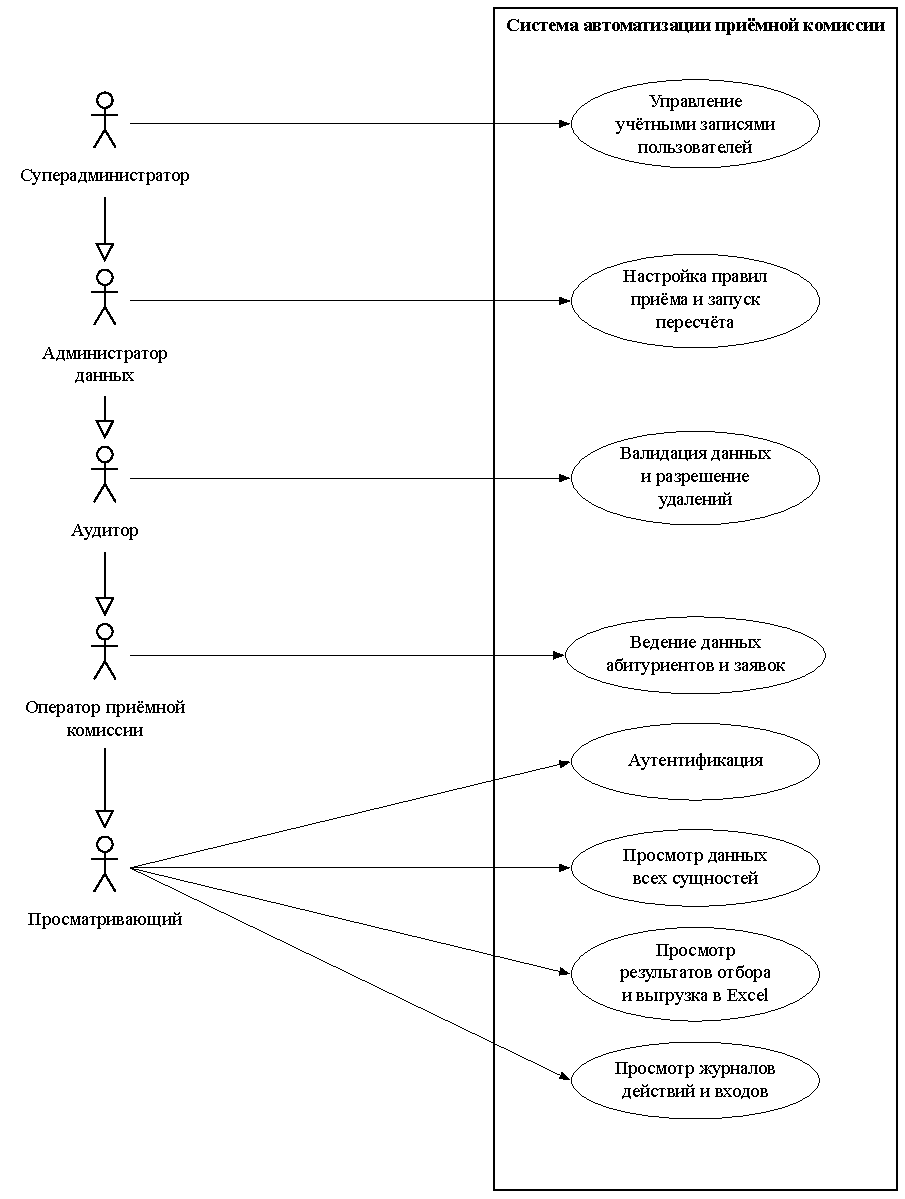
\includegraphics[width=\textwidth]{use-cases}
\caption{Диаграмма вариантов использования}
\label{fig:usecases}
\end{figure}

Соответствие категорий сценариев и ролей следующее.
Сценарий <<Аутентификация>> доступен всем пользователям, включая неаутентифицированных, и предшествует любой работе с системой.
Сценарий <<Просмотр результатов отбора и выгрузка в Excel>> и сценарий <<Просмотр журналов действий и входов>> доступны всем аутентифицированным пользователям, начиная с роли Просматривающего.
Сценарий <<Ведение данных абитуриентов и заявок>> доступен Оператору приёмной комиссии и всем ролям выше по иерархии.
Сценарий <<Валидация данных и разрешение удалений>> доступен Аудитору и всем ролям выше.
Сценарий <<Настройка правил приёма и запуск пересчёта>> объединяет управление организационной структурой, конкурсными списками, категориями приёма и группами критериев оценивания; он доступен Администратору данных и Суперадминистратору.
Сценарий <<Управление учётными записями пользователей>> доступен только Суперадминистратору.

Подробное соответствие ролей и прав на запись приведено в таблице~\ref{tab:roles} подраздела~\ref{subsec:roles}.

\subsection{Общая структура взаимодействия компонентов}

Для системы выбрана клиент-серверная архитектура с разделением обязанностей между клиентским одностраничным приложением (Single-Page Application), серверной частью REST API и реляционной базой данных.

Клиентская часть~--~одностраничное приложение, выполняемое в браузере пользователя.
Клиент взаимодействует с сервером исключительно через REST API по протоколу HTTPS, передавая данные в формате JSON.
Для аутентификации пользователя выбрана схема Bearer-токена: после успешного входа клиент сохраняет полученный JSON Web Token в локальном хранилище браузера и автоматически добавляет его в заголовок каждого последующего запроса.

Серверная часть выполняет роль REST API: принимает HTTP-запросы от клиента, выполняет проверку прав доступа, валидацию входных данных, реализует бизнес-логику и взаимодействует с базой данных.
Серверная часть не хранит состояния сессии пользователя~--~вся необходимая информация о пользователе извлекается из проверенного JWT-токена при каждом запросе.
Подобный подход обеспечивает горизонтальную масштабируемость и упрощает развёртывание системы.

База данных обеспечивает долговременное хранение всех данных приложения с поддержкой транзакционной целостности на уровне СУБД.
Управление схемой базы данных возлагается на отдельную систему миграций, что позволяет отслеживать историю изменений структуры и автоматически применять необходимые миграции при обновлении приложения.

Схема общего взаимодействия компонентов приложения представлена на рисунке~\ref{fig:architecture}.

\begin{figure}[htbp]
\centering
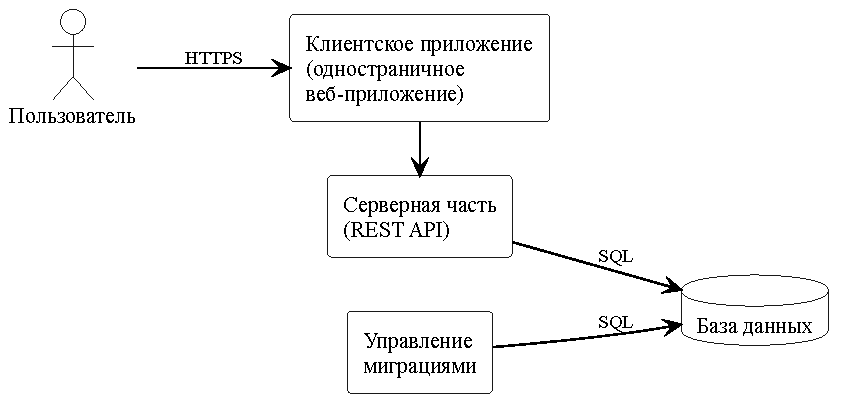
\includegraphics[width=0.9\textwidth]{architecture}
\caption{Схема взаимодействия компонентов приложения}
\label{fig:architecture}
\end{figure}

\subsection{Архитектура серверной части}

Архитектура серверной части~--~двухслойная и построена по шаблону <<репозиторий>> (Repository) из каталога шаблонов корпоративных приложений М.~Фаулера \citesrc{fowler-paa}: каждой таблице базы данных соответствует отдельный класс-репозиторий, инкапсулирующий доступ к ней, а контроллеры обращаются к репозиториям напрямую, без выделения отдельного сервисного слоя.
Подобный подход выбран сознательно: большинство операций над данными представляют собой стандартные операции CRUD, для которых введение дополнительного абстрактного слоя избыточно и приводит к разрастанию количества классов без увеличения функциональной ценности.
Бизнес-логика, выходящая за рамки CRUD (алгоритм отбора, экспорт в Excel, ведение журнала аудита), выносится в отдельные сервисы, подключаемые к репозиториям и контроллерам.

Слой контроллеров принимает HTTP-запросы, выполняет преобразование входных данных в объекты передачи данных, декларативно проверяет права доступа по роли пользователя, делегирует выполнение операции репозиторию и возвращает HTTP-ответ.
Слой репозиториев инкапсулирует доступ к базе данных, выполняет преобразование данных между типами языка реализации и типами СУБД, реализует логику CRUD-операций и вызывает сервисы аудита и пересчёта результатов отбора.

\subsection{Архитектура клиентской части}

Клиентская часть строится на основе библиотеки React с применением функциональных компонентов и хуков.
Маршрутизация выполняется средствами библиотеки декларативной маршрутизации, что позволяет компактно описать карту страниц и ограничивать доступ к ним в зависимости от роли текущего пользователя.

Глобальное состояние клиентского приложения разделяется на три независимые области: сведения о текущем пользователе и его токене доступа, текущая тема оформления (светлая или тёмная) и текущий язык интерфейса.
Каждая из областей инкапсулируется в отдельный контекст и не зависит от остальных.
Состояние, специфичное для конкретной страницы (фильтры таблицы, открытые модальные окна), хранится в локальном состоянии соответствующего компонента.

Взаимодействие с сервером выполняется через единый клиент HTTP-запросов с настроенным базовым адресом API.
На клиент устанавливаются перехватчики запросов и ответов, обеспечивающие: автоматическое добавление заголовка \code{Authorization: Bearer <token>} ко всем исходящим запросам; добавление заголовка \code{Accept-Language} с текущим языком интерфейса; обработку ошибки 401 (Unauthorized) с автоматическим переходом на страницу входа.

\subsection{Проектирование базы данных}

\subsubsection{Метод проектирования}

Для проектирования базы данных выбран классический подход <<сверху вниз>>: на основе анализа предметной области строится концептуальная модель данных, которая последовательно детализируется до логической и физической моделей.
Схема базы данных описывается набором SQL-сценариев, объединённых в один changelog-файл формата YAML под управлением системы миграций.
Подобный подход обеспечивает полный контроль над структурой и индексами базы данных, делает все изменения схемы явными и отслеживаемыми в системе контроля версий, а также гарантирует идентичность схемы в средах разработки, тестирования и эксплуатации.

\subsubsection{Концептуальная модель}

В концептуальной модели выделены следующие группы сущностей.

Организационная иерархия: факультет содержит кафедры, кафедра содержит специальности.
Для каждой специальности определены один или несколько конкурсных списков (бюджет, платное, целевое направление), каждый конкурсный список разделён на категории приёма с указанием квоты и приоритета защиты.

Критерии оценивания: для каждого конкурсного списка определена группа критериев оценивания (например, средний балл аттестата, баллы централизованного тестирования по предметам).
Группа состоит из критериев, упорядоченных по приоритету для лексикографической сортировки кандидатов.

Абитуриенты: каждый абитуриент имеет идентификатор, имя, оценки по критериям и список заявок в категории приёма с указанием приоритета предпочтения.
Для каждого абитуриента сохраняется булевый признак валидации данных вторым пользователем.

Результаты отбора: итоговая таблица содержит идентификаторы абитуриентов и категорий, в которые они зачислены.
Таблица полностью перестраивается алгоритмом пересчёта при любом изменении входных данных.

Подсистемы аудита и логического удаления: журнал действий пользователей, журнал попыток входа в систему, запросы на удаление абитуриентов с двухступенчатым подтверждением.

ER-диаграмма базы данных представлена на рисунке~\ref{fig:erdiagram}.

\begin{figure}[htbp]
\centering
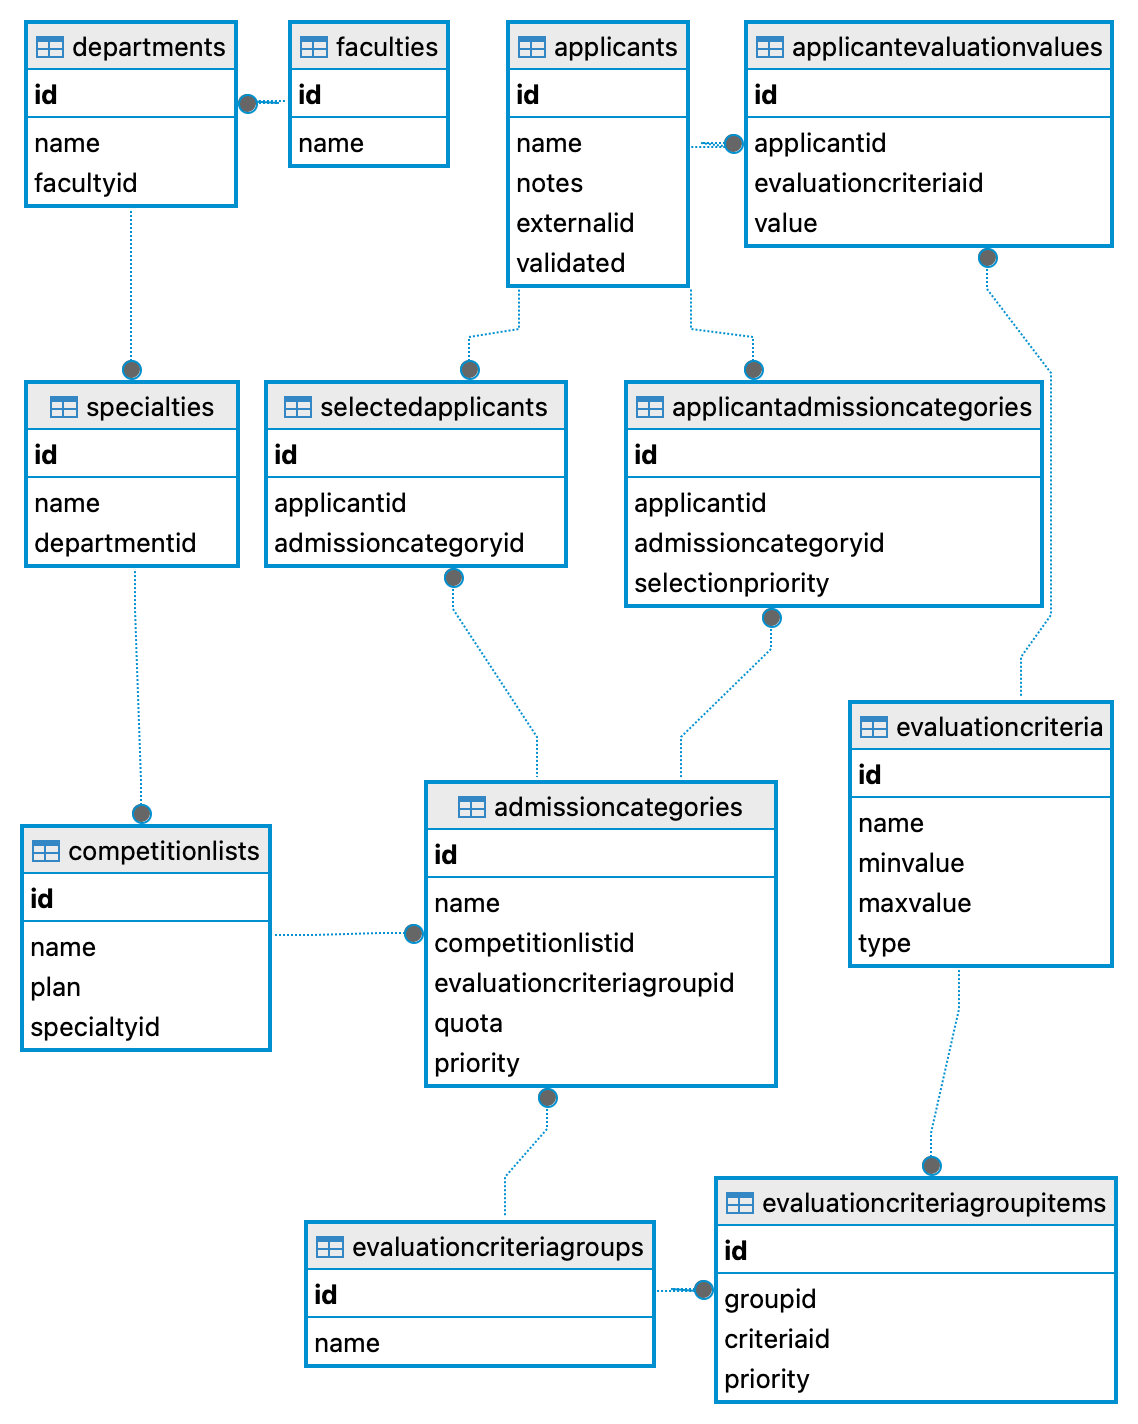
\includegraphics[width=\linewidth,keepaspectratio]{er}
\caption{ER-диаграмма базы данных}
\label{fig:erdiagram}
\end{figure}

\subsubsection{Логическая модель}

Логическая модель базы данных нормализована до третьей нормальной формы.
Ключевые таблицы и их связи приведены в таблице~\ref{tab:tables}.

\begin{longtblr}[
  caption = {Основные таблицы базы данных},
  label = {tab:tables},
]{
  colspec = {|Q[l]|X|},
  width = \textwidth,
  hlines, vlines,
  rowhead = 1,
  row{1} = {halign=c},
}
Таблица & Назначение \\
\code{faculties} & Факультеты университета \\
\code{departments} & Кафедры, связь с факультетом по внешнему ключу \\
\code{specialties} & Специальности, связь с кафедрой по внешнему ключу \\
\code{competitionlists} & Конкурсные списки специальности с общим планом приёма \\
\code{admissioncategories} & Категории приёма с квотой и приоритетом защиты \\
\code{evaluationcriteria} & Критерии оценивания с диапазоном и выбором варианта <<больше~--~лучше>> или <<меньше~--~лучше>> \\
\code{evaluationcriteriagroups} & Группы критериев \\
\code{evaluationcriteriagroupitems} & Связь группы и критерия с приоритетом для сортировки \\
\code{applicants} & Абитуриенты с признаком валидации данных \\
\code{applicantevaluationvalues} & Оценки абитуриентов по критериям \\
\code{applicantadmissioncategories} & Заявки абитуриентов в категории с приоритетом предпочтения \\
\code{selectedapplicants} & Итоговые результаты отбора \\
\code{users} & Учётные записи операторов с ролью и признаком активности \\
\code{audit\_log} & Журнал действий пользователей \\
\code{auth\_log} & Журнал попыток входа в систему \\
\code{applicant\_deletion\_requests} & Запросы на удаление абитуриентов \\
\end{longtblr}

Для таблицы \code{applicantevaluationvalues} предусмотрено уникальное ограничение по паре столбцов \code{(applicant\_id, evaluation\_criteria\_id)}, что гарантирует невозможность хранения двух оценок одного абитуриента по одному критерию.
В таблице \code{applicants} предусмотрен булевый столбец \code{validated} для хранения статуса валидации данных вторым пользователем.

\subsection{Ролевая модель доступа}
\label{subsec:roles}

В системе определены пять ролей пользователей, отличающихся набором прав на запись данных.
Все аутентифицированные пользователи имеют право чтения всех данных.
Соответствие ролей и прав на запись приведено в таблице~\ref{tab:roles}.

\begin{longtblr}[
  caption = {Ролевая модель доступа},
  label = {tab:roles},
]{
  colspec = {|Q[l,wd=4.5cm]|X|},
  width = \textwidth,
  hlines, vlines,
  rowhead = 1,
  row{1} = {halign=c},
}
Роль & Права на запись \\
\code{SuperAdmin} & Все операции, включая управление учётными записями пользователей \\
\code{DataAdministrator} & Структура университета, абитуриенты, аудит, кроме управления пользователями \\
\code{Auditor} & Абитуриенты, валидация данных, подтверждение и отклонение запросов на удаление \\
\code{AdmissionsOperator} & Только данные абитуриентов и их заявок в категории \\
\code{DataViewer} & Только чтение, без прав записи \\
\end{longtblr}

Проверка прав доступа выполняется на серверной части декларативно: каждый метод обработчика помечается требуемой ролью, и попытки вызова метода пользователем с недостаточными правами отклоняются ещё до выполнения бизнес-логики.
На клиентской части все аутентифицированные пользователи видят одинаковый набор страниц, но кнопки выполнения операций скрываются в зависимости от роли текущего пользователя.

\subsection{Алгоритм пересчёта результатов отбора}

Центральным элементом проекта является алгоритм автоматического распределения абитуриентов по категориям приёма.
Алгоритм реализует принцип deferred acceptance \citesrc{gale} с вытеснением слабых кандидатов \citesrc{roth} и состоит из двух фаз: проверка квоты категории и проверка общего плана конкурсного списка.

\subsubsection{Этапы алгоритма}

Этап~1. Предварительная фильтрация.
Из множества заявок исключаются те, для которых у абитуриента не заполнен хотя бы один критерий из группы критериев, привязанной к категории.
Подобные заявки никогда не будут учтены при отборе, поэтому их фильтрация на ранней стадии сокращает объём обрабатываемых данных.

Этап~2. Инициализация.
Все абитуриенты с непустыми списками заявок помещаются в очередь обработки.
Для каждого абитуриента строится упорядоченный по полю \code{selectionpriority} список предпочтений между категориями.

Этап~3. Основной цикл.
Из очереди извлекается очередной абитуриент.
Из его списка предпочтений берётся следующая по приоритету категория.
Абитуриент добавляется в пул кандидатов этой категории.
Пул~--~упорядоченное множество с компаратором, упорядочивающим кандидатов по убыванию <<силы>>.

Этап~4. Проверка квоты категории.
Если после добавления нового кандидата размер пула категории превысил её квоту, из пула извлекается самый слабый кандидат~--~максимальный элемент множества при компараторе по убыванию.
Извлечённый кандидат возвращается в очередь обработки, и его указатель текущего предпочтения смещается на следующую категорию.

Этап~5. Проверка общего плана конкурсного списка.
Если суммарное количество кандидатов во всех категориях одного конкурсного списка превысило его план, из категории с наибольшим значением \code{priority} (наименее защищённой) извлекается самый слабый кандидат и возвращается в очередь.

Этап~6. Завершение.
Алгоритм завершается, когда очередь обработки становится пустой.
Содержимое всех пулов категорий копируется в таблицу \code{selectedapplicants} массовой операцией после полной очистки таблицы.

\subsubsection{Асимптотическая сложность алгоритма}

Каждая заявка обрабатывается не более одного раза при первом извлечении из очереди и не более одного раза при каждом возможном вытеснении, что даёт оценку общего числа операций с пулами, пропорциональную произведению числа абитуриентов на среднее число заявок одного абитуриента.
Операции вставки, удаления и чтения максимума в упорядоченном множестве выполняются за логарифмическое время от размера пула, а построение вектора оценок одного кандидата~--~за время, пропорциональное числу критериев в группе.

Итоговая временная сложность алгоритма выражается формулой~\ref{eq:time-complexity}:

\begin{equation}
\label{eq:time-complexity}
T = O(N \cdot M \cdot (\log K + R)),
\end{equation}

\begin{explanationx}
\item где $\mathrm{N}$~--~число абитуриентов;
\item $\mathrm{M}$~--~среднее число заявок одного абитуриента;
\item $\mathrm{K}$~--~максимальный размер пула категории, ограниченный её квотой;
\item $\mathrm{R}$~--~число критериев в группе категории.
\end{explanationx}

Затраты памяти определяются хранением очереди обработки, списков предпочтений абитуриентов и пулов категорий и выражаются формулой~\ref{eq:space-complexity}:

\begin{equation}
\label{eq:space-complexity}
S = O(N \cdot M).
\end{equation}

\subsubsection{Ранжирование кандидатов}

Компаратор кандидатов сравнивает их лексикографически по следующим параметрам в указанном порядке: вектор оценок по критериям категории по убыванию; значение \code{selectionpriority} заявки по возрастанию (более высокий приоритет предпочтения~--~меньшее число); идентификатор абитуриента по возрастанию (для обеспечения детерминированности и уникальности элементов упорядоченного множества).

Для критериев с вариантом \code{lower\_is\_better} значение инвертируется (умножается на минус единицу) перед сравнением, что позволяет использовать единый компаратор по принципу <<больше~--~лучше>>.

Блок-схема алгоритма представлена на рисунке~\ref{fig:selection-algo}.

\begin{figure}[htbp]
\centering
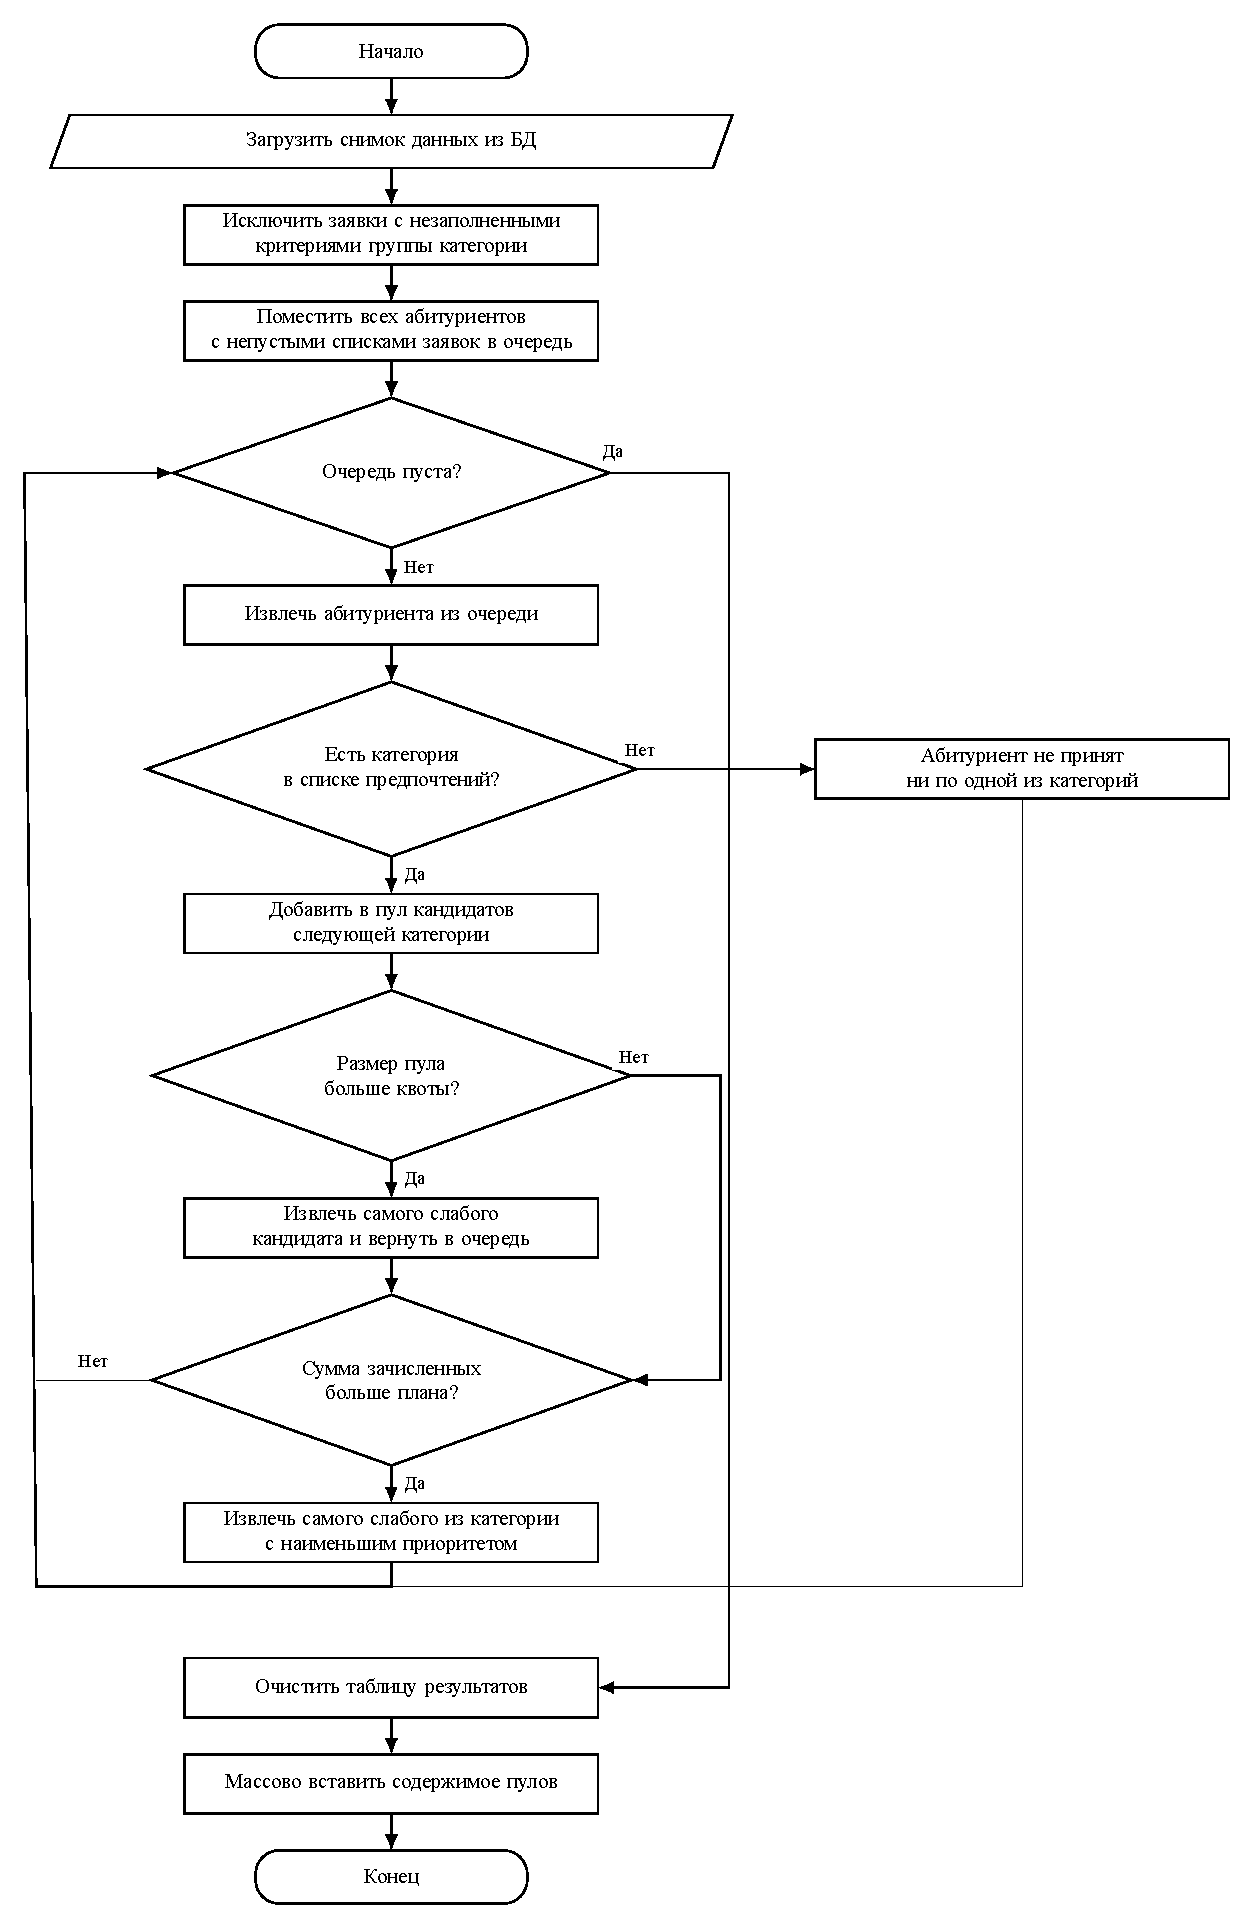
\includegraphics[width=\textwidth]{selection-algorithm}
\caption{Блок-схема алгоритма пересчёта результатов отбора}
\label{fig:selection-algo}
\end{figure}

\subsection{Архитектура подсистемы аудита и логического удаления}

\subsubsection{Журнал действий}

Подсистема аудита~--~единая точка записи действий пользователей, общая для всех репозиториев.
При выполнении любой операции записи репозиторий вызывает сервис аудита, который формирует запись в таблице \code{audit\_log}.
Состав полей таблицы приведён в таблице~\ref{tab:auditlog}.

\begin{longtblr}[
  caption = {Состав полей таблицы журнала действий},
  label = {tab:auditlog},
]{
  colspec = {|Q[l]|X|},
  width = \textwidth,
  hlines, vlines,
  rowhead = 1,
  row{1} = {halign=c},
}
Поле & Назначение \\
\code{id} & Первичный ключ записи \\
\code{user\_id} & Идентификатор пользователя, выполнившего действие \\
\code{username} & Имя пользователя на момент действия (на случай переименования) \\
\code{action} & Код действия \\
\code{entity\_type} & Тип изменённой сущности \\
\code{entity\_id} & Строковый идентификатор изменённой сущности \\
\code{changes} & Содержание изменения в формате JSONB \\
\code{created\_at} & Момент выполнения действия в часовом поясе UTC \\
\end{longtblr}

Поле \code{action} принимает одно из значений: \code{create} (создание), \code{update} (обновление), \code{delete} (запрос на удаление абитуриента или удаление иной сущности), \code{validate} (подтверждение валидации абитуриента), \code{invalidate} (снятие или автоматический сброс валидации), \code{delete\_confirmed} (подтверждение запроса на удаление), \code{delete\_rejected} (отклонение запроса на удаление), \code{recalculate\_all} (запуск пересчёта результатов отбора).

Поле \code{changes} содержит сериализованный объект с одним из трёх вариантов структуры: \code{\{after: \dots\}}~--~для создания (фиксируется состояние после изменения), \code{\{diff: \dots\}}~--~для обновления (фиксируется разница между состояниями до и после), \code{\{before: \dots\}}~--~для удаления (фиксируется состояние до изменения).
Такая структура позволяет восстановить любое состояние сущности по цепочке записей журнала.

\subsubsection{Сброс статуса валидации}

При любом изменении данных абитуриента сервис аудита автоматически сбрасывает поле \code{validated} в значение \code{false}, если оно ранее было установлено в \code{true}.
Одновременно в журнал записывается событие \code{invalidate} с признаком автоматического сброса, что позволяет отличать его от ручного снятия валидации пользователем.
Такое поведение реализует требование двойного контроля, сформулированное в подразделе~1.2.2: внесение и подтверждение данных выполняются двумя разными пользователями, а любое последующее изменение данных снова требует подтверждения.

Полный сценарий двойного контроля представлен на диаграмме деятельности, приведённой на рисунке~\ref{fig:activity-validation}.
На диаграмме выделены три дорожки: действия оператора приёмной комиссии, автоматические действия системы и действия аудитора.
Поток начинается с первичного ввода данных оператором, проходит через автоматическое сохранение с \code{validated = false} и пересчёт результатов отбора, затем переходит к проверке аудитором с принятием решения о подтверждении валидации.
Замыкающая ветвь показывает поведение системы при последующем изменении данных: автоматический сброс валидации и возврат записи на повторную проверку.

\begin{figure}[htbp]
\centering
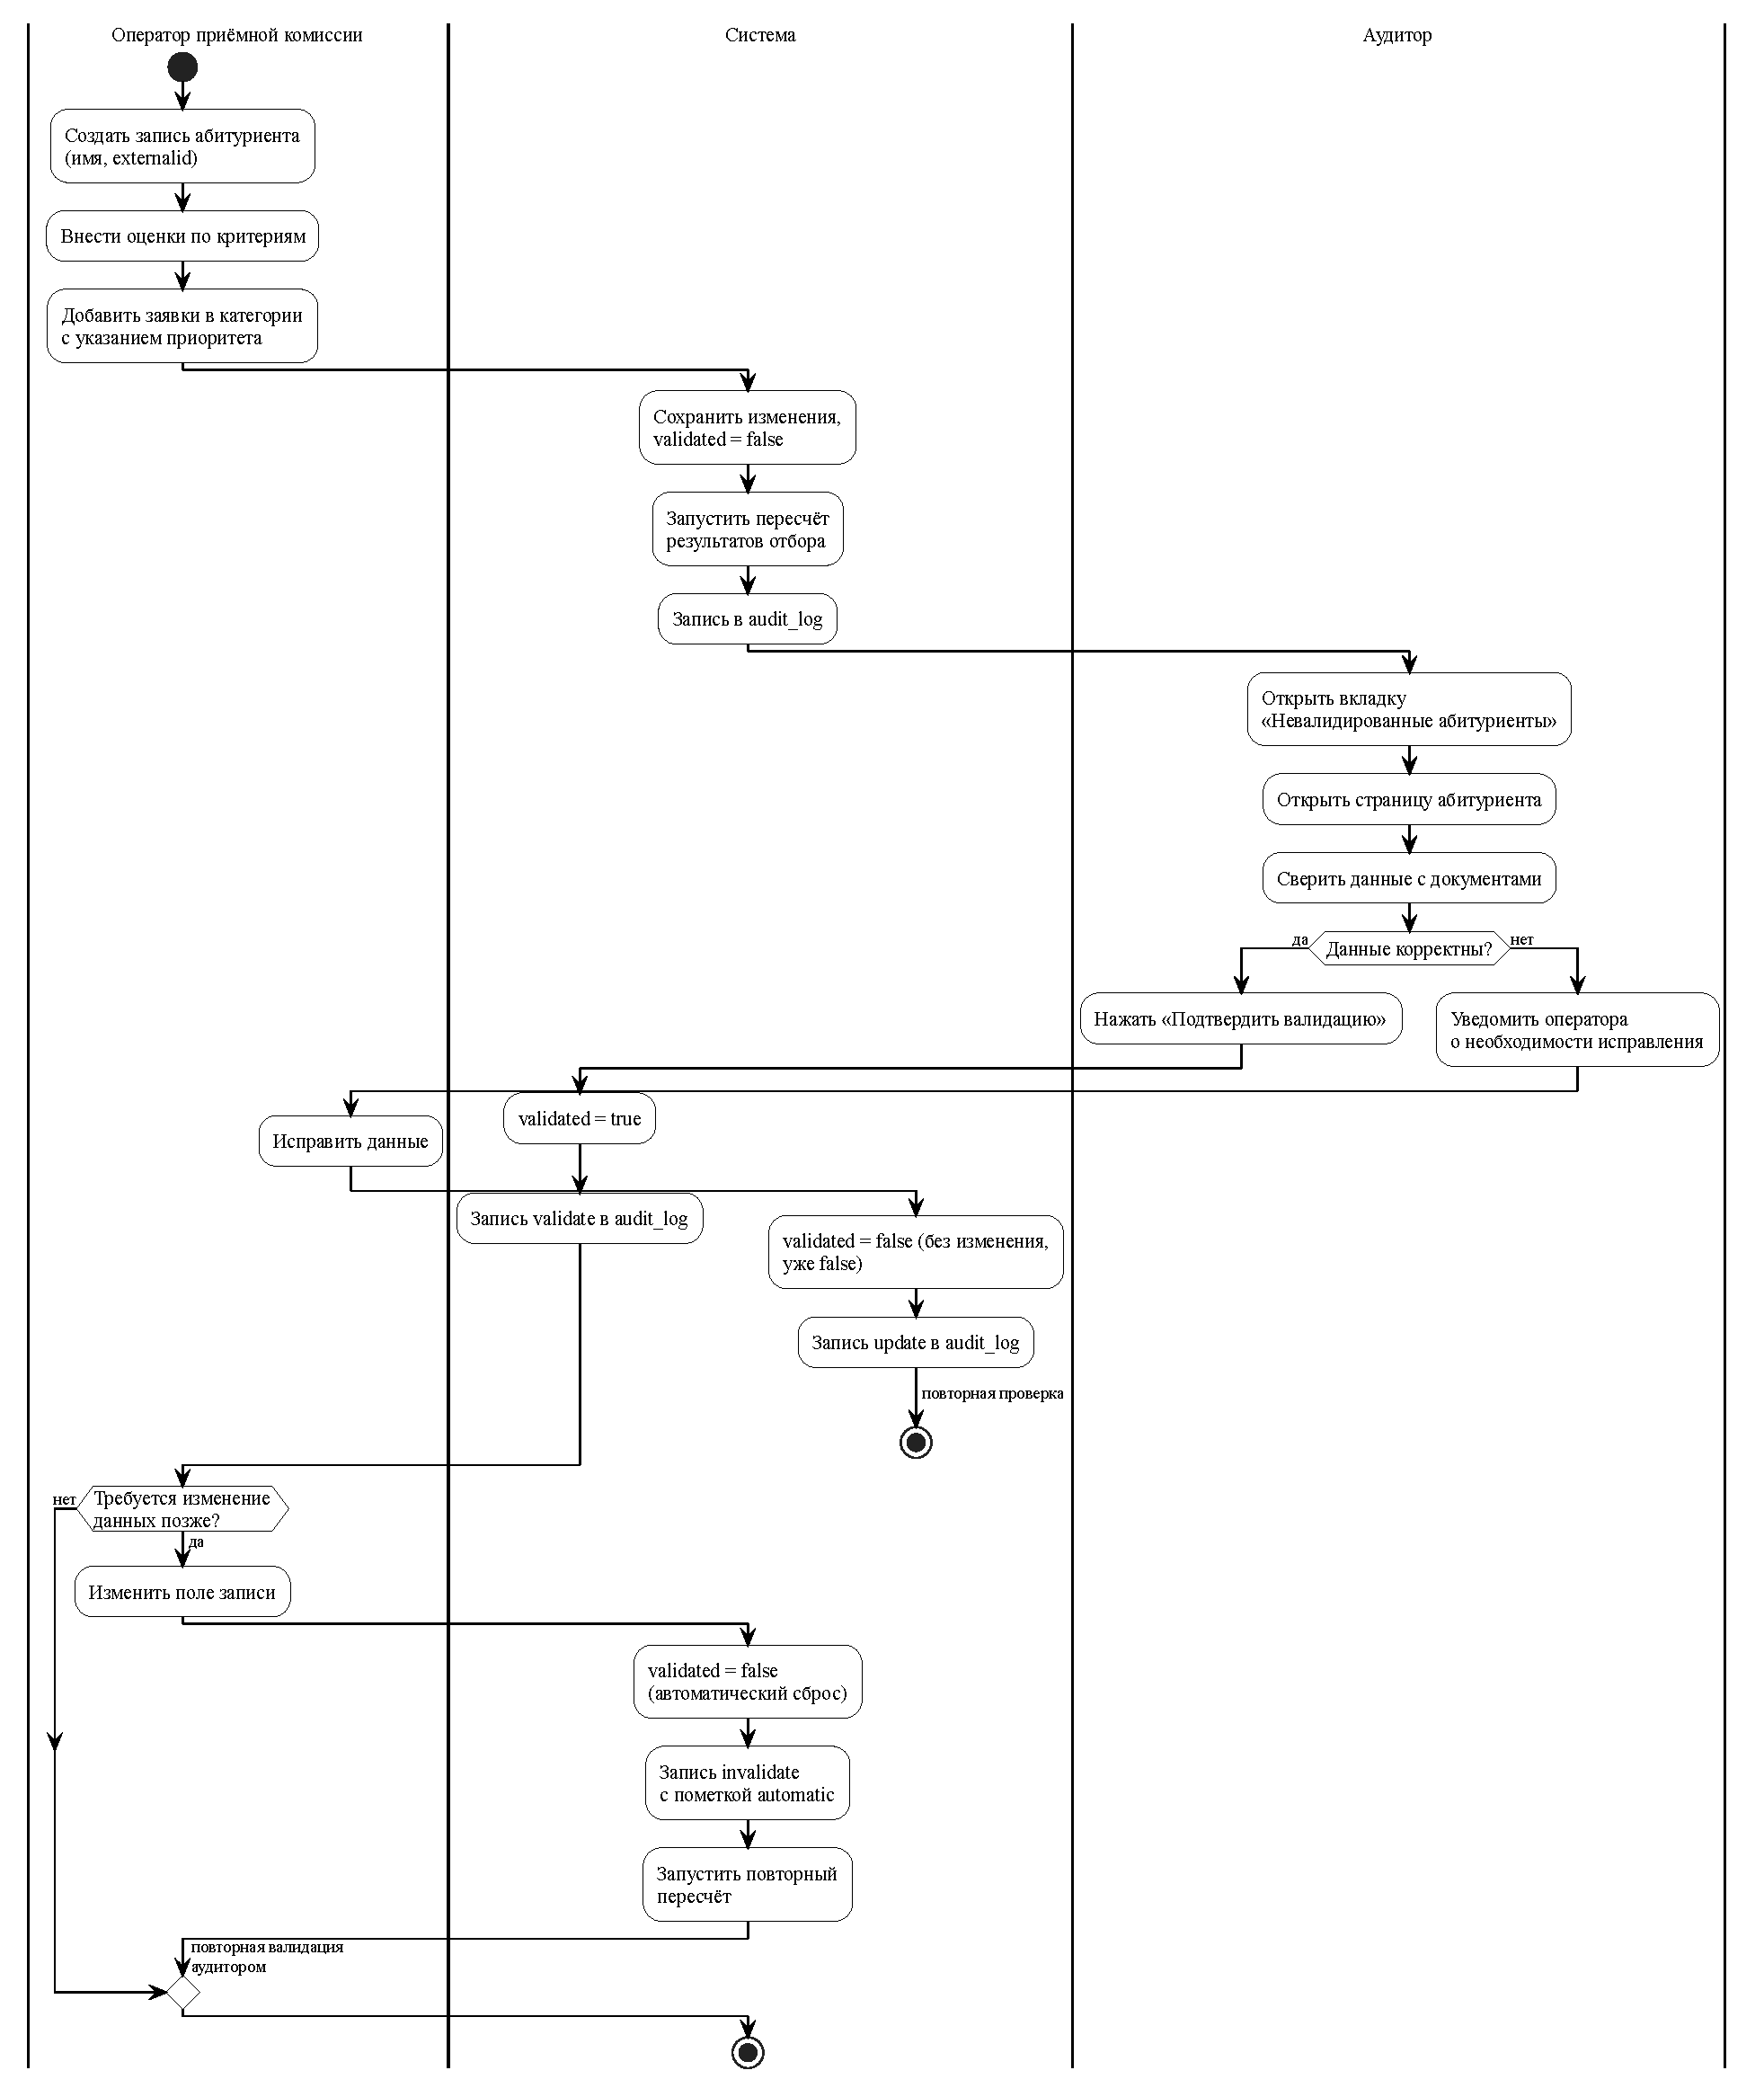
\includegraphics[width=\textwidth]{activity-validation}
\caption{Диаграмма деятельности процесса двойного контроля данных абитуриента}
\label{fig:activity-validation}
\end{figure}

\subsubsection{Двухступенчатое удаление абитуриентов}

Двухступенчатое удаление абитуриентов основано на отдельной таблице \code{applicant\_deletion\_requests} с полем \code{status}, принимающим одно из трёх значений: \code{pending} (запрос подан, ожидает решения), \code{confirmed} (запрос подтверждён), \code{rejected} (запрос отклонён).
Возможные переходы между состояниями приведены в таблице~\ref{tab:deletionstates}.

\begin{longtblr}[
  caption = {Переходы состояний запроса на удаление абитуриента},
  label = {tab:deletionstates},
]{
  colspec = {|Q[l]|Q[l]|X|},
  width = \textwidth,
  hlines, vlines,
  rowhead = 1,
  row{1} = {halign=c},
}
Из состояния & В состояние & Условие перехода \\
(отсутствует) & \code{pending} & Пользователь с правом \code{WriteApplicants} нажал <<Удалить>> \\
\code{pending} & \code{confirmed} & Пользователь с правом \code{WriteAudit} подтвердил запрос \\
\code{pending} & \code{rejected} & Пользователь с правом \code{WriteAudit} отклонил запрос \\
\code{rejected} & (отсутствует) & Возможно создание нового запроса на того же абитуриента \\
\end{longtblr}

Абитуриент со статусом запроса \code{pending} или \code{confirmed} исключается из всех выборок репозитория абитуриентов и из снимка базы данных при пересчёте результатов отбора, что обеспечивает мгновенный эффект первичного запроса на удаление без потери данных.

При переводе запроса из состояния \code{pending} в \code{rejected} дополнительно выполняется сброс поля \code{validated} абитуриента в значение \code{false} и запуск повторного пересчёта результатов отбора с включением возвращённого в активные данные абитуриента.
Перевод запроса из состояния \code{pending} в \code{confirmed} не требует пересчёта, так как абитуриент уже был исключён из снимка при подаче запроса.
        % 3 ПРОЕКТИРОВАНИЕ ПРИЛОЖЕНИЯ
\section{Программная реализация}

В соответствии с архитектурой, описанной в разделе~3, программная часть проекта была реализована в виде двух независимо собираемых частей: серверного приложения на платформе ASP.NET~Core и клиентского одностраничного приложения на библиотеке React.
Сборка серверного приложения выполняется командой \code{dotnet build}, клиентского~--~командой \code{npm run build}.
База данных управляется через инструмент Liquibase, миграции применяются автоматически при первом запуске контейнера.

\subsection{Структура серверной части}

Серверная часть приложения сгруппирована по подкаталогам в соответствии с назначением входящих в них классов.

Каталог \code{Controllers} содержит REST-контроллеры, по одному на каждую группу сущностей.
Каждый контроллер наследуется от \code{ControllerBase}, помечен атрибутом \code{[ApiController]} и атрибутом маршрутизации \code{[Route("api/v1/...")]}.
Для простых CRUD-операций контроллер делегирует выполнение соответствующему репозиторию напрямую.
Для составных операций~--~таких как запрос на удаление абитуриента, подтверждение или отклонение запроса, валидация данных~--~контроллер выступает оркестратором: координирует обращения к нескольким репозиториям, извлекает идентификатор текущего пользователя из утверждений JWT и при необходимости инициирует пересчёт результатов отбора через \code{SelectionService}.

Каталог \code{Repositories} содержит репозитории, по одному на каждую таблицу базы данных.
Репозитории работают с базой данных через драйвер Npgsql, выполняя параметризованные SQL-запросы.
Каждый репозиторий поддерживает базовый набор операций CRUD, а также специфичные для предметной области операции (например, \code{GetByFacultyAsync}, \code{GetPagedAsync}).

Каталог \code{Services} содержит сервисы, реализующие бизнес-логику, выходящую за рамки CRUD: \code{JwtService} для генерации и валидации JSON Web Tokens; \code{SelectionService} для пересчёта результатов отбора; \code{ExcelExportService} для формирования файлов Excel; \code{AuditLogger} для записи журнала действий пользователей; \code{AuthLogger} для записи журнала попыток входа; \code{CurrentUserService} для получения сведений о текущем пользователе из утверждений (claims) JWT.

Каталог \code{Dtos} содержит объекты передачи данных, разделённые на подкаталоги \code{Requests} (входящие данные) и \code{Responses} (исходящие данные).
Для постраничной выдачи используется обобщённый тип \code{PagedResponse<T>}.

Каталог \code{Constants} содержит вспомогательные классы констант, в том числе \code{UserRoles} с предопределёнными строками для атрибута авторизации.

Каталог \code{Resources} содержит маркерный класс \code{SharedResources} и файлы ресурсов \code{SharedResources.ru.resx} и \code{SharedResources.en.resx} с переводами сообщений об ошибках.

\subsection{Регистрация сервисов и конфигурация приложения}

Все сервисы и репозитории регистрируются в контейнере зависимостей в файле \code{Program.cs}.
Файл также настраивает: подключение к базе данных PostgreSQL через строку соединения из конфигурации; аутентификацию по JWT с алгоритмом HS256 и валидацией издателя, времени жизни и подписи токена; авторизацию с предопределёнными политиками для каждой роли; локализацию с поддержкой языков \code{ru} (по умолчанию) и \code{en}; CORS-политику, разрешающую запросы от настроенных в конфигурации источников с обязательным экспонированием заголовка \code{Content-Disposition} (необходим для скачивания файлов Excel).

При первом запуске приложения, если в базе данных не существует ни одного пользователя, выполняется создание учётной записи администратора с именем пользователя и паролем, заданными в переменных окружения \code{InitialAdmin\_\_Username} и \code{InitialAdmin\_\_Password} (значения по умолчанию~--~\code{admin} и \code{Admin@123}).
Учётной записи присваивается роль \code{SuperAdmin}.

\subsection{Реализация аутентификации и авторизации}

Аутентификация реализована в контроллере \code{AuthController}, эндпоинт \code{POST /api/v1/auth/login}.
Контроллер принимает имя пользователя и пароль, выполняет поиск учётной записи в базе данных, проверяет хеш пароля и, в случае успеха, генерирует JSON Web Token через сервис \code{JwtService}.
Токен содержит утверждения с идентификатором пользователя, именем пользователя и ролью; срок действия токена~--~8 часов.
Параллельно с генерацией токена сервис \code{AuthLogger} записывает успешную попытку входа в таблицу \code{auth\_log}.
Полный текст сервиса \code{JwtService.cs} приведён в приложении~А.
При неуспешной попытке (несуществующий пользователь, неверный пароль, заблокированная учётная запись) также делается запись в журнал с соответствующим статусом.

Авторизация реализована декларативно через атрибуты на уровне методов контроллеров.
Для удобства использования в классе \code{UserRoles} определены строковые константы, соответствующие группам ролей с одинаковыми правами: \code{SuperAdmin}, \code{WriteStructure} (SuperAdmin плюс DataAdministrator), \code{WriteApplicants} (SuperAdmin, DataAdministrator, Auditor, AdmissionsOperator), \code{WriteAudit} (SuperAdmin, DataAdministrator, Auditor).
Например, метод создания факультета помечен атрибутом \code{[Authorize(Roles = UserRoles.WriteStructure)]}.

\subsection{Реализация алгоритма пересчёта результатов отбора}

Алгоритм пересчёта результатов отбора реализован в сервисе \code{SelectionService} с разделением на координирующий метод \code{RecalculateAllAsync} и чистую in-memory логику в статическом классе \code{FullRecalculationCore}.
Такое разделение позволяет проверить алгоритм юнит-тестами на готовом снимке без подключения к базе данных.

Метод \code{RecalculateAllAsync} выполняет последовательность действий: открывает транзакцию к базе данных через \code{NpgsqlConnection.BeginTransactionAsync}; захватывает глобальную транзакционную блокировку через функцию \code{pg\_advisory\_xact\_lock(0)}, что исключает параллельный пересчёт при одновременном обновлении данных несколькими пользователями; загружает снимок базы данных шестью пакетными SQL-запросами (по одному на тип сущности~--~заявки, категории, планы, критерии групп, оценки, типы критериев), исключая итеративное обращение к базе данных в цикле по записям; передаёт снимок в метод \code{FullRecalculationCore.Run}; полностью очищает таблицу \code{selectedapplicants}; массово вставляет результат через операцию \code{COPY BINARY} для достижения максимальной производительности; записывает в журнал аудита событие \code{recalculate\_all}; подтверждает транзакцию.

Для массовой вставки результата использован интерфейс \code{NpgsqlBinaryImporter}, экспортируемый методом \code{BeginBinaryImportAsync} драйвера Npgsql; формат вставки~--~бинарный, что устраняет накладные расходы на разбор текстовых представлений значений на стороне сервера базы данных.
Полный текст модуля \code{SelectionService.cs} приведён в приложении~А.

Метод \code{FullRecalculationCore.Run} реализует алгоритм очереди с вытеснением, описанный в разделе~3.7.
Метод чист: на одинаковом входе всегда производит одинаковый выход, что упрощает написание юнит-тестов.
Полный текст модуля \code{FullRecalculationCore.cs} приведён в приложении~А.
Сравнение кандидатов в пуле категории выполняется компаратором \code{CategoryComparer}, реализующим интерфейс \code{IComparer<Candidate>}.
Компаратор спроектирован так, чтобы максимум \code{SortedSet} соответствовал наиболее слабому кандидату~--~это упрощает операцию вытеснения, выполняемую при превышении квоты.
Полный текст модуля \code{CategoryComparer.cs} приведён в приложении~А.

Для критериев с направлением оптимизации \code{lower\_is\_better} значение умножается на минус единицу при построении вектора оценок, что позволяет использовать единый компаратор по принципу <<больше~--~лучше>> без ветвления внутри сравнения.

\subsection{Реализация подсистемы аудита}

Сервис \code{AuditLogger} реализует интерфейс \code{IAuditLogger}, состав методов которого приведён в таблице~\ref{tab:auditlogger}.

\begin{longtblr}[
  caption = {Методы интерфейса IAuditLogger},
  label = {tab:auditlogger},
]{
  colspec = {|Q[l,wd=6.5cm]|X|},
  width = \textwidth,
  hlines, vlines,
  rowhead = 1,
  row{1} = {halign=c},
}
Метод & Назначение \\
\code{LogCreateAsync} & Запись действия \code{create} с состоянием после изменения \\
\code{LogUpdateAsync} & Запись действия \code{update} с разностью состояний до и после \\
\code{LogDeleteAsync} & Запись действия \code{delete} с состоянием до изменения \\
\code{LogValidateAsync} & Запись действия \code{validate} (ручное подтверждение валидации) \\
\code{LogInvalidateAsync} & Запись действия \code{invalidate} с пометкой ручного или автоматического сброса \\
\code{LogDeleteConfirmedAsync} & Запись действия \code{delete\_confirmed} \\
\code{LogDeleteRejectedAsync} & Запись действия \code{delete\_rejected} \\
\code{LogRecalculationAsync} & Запись действия \code{recalculate\_all} с числом зачисленных \\
\code{ResetValidationIfNeededAsync} & Условный сброс поля \code{validated} при изменении данных абитуриента \\
\end{longtblr}

Сервис внедряется во все репозитории и сервисы, выполняющие изменения данных, через конструктор.
Внутренний метод \code{WriteAsync} формирует параметризованный SQL-запрос \code{INSERT INTO audit\_log} с приведением поля \code{changes} к типу \code{jsonb} непосредственно в строке запроса, что устраняет необходимость преобразования параметра на стороне приложения.
Идентификатор и имя пользователя извлекаются из сервиса \code{ICurrentUserService}, который читает соответствующие \code{Claims} из текущего \code{HttpContext}.

Метод \code{ResetValidationIfNeededAsync} проверяет текущее значение поля \code{validated} абитуриента и выполняет обновление только в случае, когда оно равно \code{true}, что исключает избыточные записи в журнал при изменении данных уже невалидированного абитуриента.
При сбросе автоматически записывается событие \code{invalidate} с пометкой \code{automatic = true}, отделяющей автоматический сброс от явного снятия валидации пользователем.

Для просмотра журнала действий предусмотрен контроллер \code{AuditController} с эндпоинтом \code{GET /audit/log}, поддерживающим фильтрацию по дате, действию, типу сущности и пользователю, а также эндпоинт \code{GET /audit/entity-history}, возвращающий полную историю изменений конкретной сущности.
Полный текст модуля \code{AuditLogger.cs} приведён в приложении~А.

\subsection{Реализация логического удаления абитуриентов}

Двухступенчатое удаление реализовано через таблицу \code{applicant\_deletion\_requests}.
При вызове метода \code{DELETE /applicants/\{id\}} репозиторий создаёт в таблице запись со статусом \code{pending}, связывая её с идентификатором текущего пользователя и идентификатором абитуриента.
После этого вызывается \code{SelectionService.RecalculateAllAsync}, который при формировании снимка исключает абитуриентов с активными запросами на удаление.

Для подтверждения и отклонения запросов реализованы эндпоинты \code{POST /audit/pending-deletions/\{id\}/confirm} и \code{POST /audit/pending-deletions/\{id\}/reject}, доступные пользователям с правом \code{WriteAudit}.
При подтверждении статус запроса меняется на \code{confirmed}, и абитуриент остаётся скрытым из всех выборок.
При отклонении статус меняется на \code{rejected}, флаг валидации абитуриента сбрасывается в значение \code{false}, и запускается повторный пересчёт результатов отбора с включением вернувшегося абитуриента.
После отклонения возможно создание нового запроса на удаление того же абитуриента.

\subsection{Структура клиентской части}

Клиентская часть структурирована по принципу разделения по типу содержимого.

Каталог \code{src/api} содержит модули, инкапсулирующие вызовы REST API.
Каждый модуль соответствует одной группе эндпоинтов сервера: \code{authApi.js}, \code{applicantsApi.js}, \code{facultyApi.js} и так далее.
Все модули используют единый экземпляр Axios, настроенный в файле \code{src/api/index.js}.

Каталог \code{src/pages} содержит компоненты страниц, отображаемых по разным маршрутам: \code{Login.jsx}, \code{Applicants.jsx}, \code{Faculties.jsx} и другие.
Маршрутизация описана в файле \code{src/AppRouter.jsx} с использованием библиотеки React~Router.

Каталог \code{src/components} содержит переиспользуемые компоненты: \code{ContentHeader} с переключателем языка, \code{ProtectedRoute} для защиты маршрутов по роли, общие компоненты таблиц и форм.

Каталог \code{src/contexts} содержит провайдеры глобальных контекстов: \code{AuthContext}, \code{ThemeContext}, \code{LanguageContext}.

Каталог \code{src/hooks} содержит пользовательские хуки, в том числе \code{usePermissions}, возвращающий булевые флаги для проверки прав пользователя на запись.

Каталог \code{src/i18n} содержит конфигурацию библиотеки react-i18next и файлы переводов \code{locales/ru/translation.json}, \code{locales/en/translation.json}.

\subsection{Интерцептор Axios}

Интерцептор запроса, настроенный на едином экземпляре Axios, прикрепляет к каждому исходящему запросу заголовок \code{Authorization: Bearer <token>}, считывая токен из локального хранилища браузера по ключу \code{auth}.
Также интерцептор добавляет заголовок \code{Accept-Language} со значением языка из локального хранилища по ключу \code{language}~--~это позволяет серверу выбирать нужный язык сообщений об ошибках.
Чтение языка из локального хранилища напрямую (без использования React-хуков) обусловлено тем, что хуки React недоступны в интерцепторах Axios.
Полный текст модуля \code{api/index.js} с реализацией интерцепторов приведён в приложении~А.

Интерцептор ответа обрабатывает HTTP-статус 401 (Unauthorized): при его получении интерцептор очищает локальное хранилище и перенаправляет пользователя на страницу входа.
Это обеспечивает корректное поведение приложения при истечении срока действия токена.

\subsection{Хук серверной пагинации таблиц}

Все таблицы клиентской части обязаны использовать серверную пагинацию и серверные фильтры~--~это требование к проекту обусловлено невозможностью загружать в браузер десятки тысяч записей абитуриентов целиком.
Для централизации этого поведения разработан пользовательский хук \code{useServerTable}, инкапсулирующий состояние пагинации, фильтров, сортировки и загрузки.

Хук принимает на вход стабильную (обёрнутую в \code{useCallback}) функцию запроса данных и возвращает объект с текущими значениями состояния, обработчиком события изменения таблицы и подготовленным объектом параметра \code{pagination} для компонента \code{Table} библиотеки Ant Design.
При изменении страницы, размера страницы, фильтров или сортировки хук автоматически запускает повторный запрос с актуальными параметрами.
Применение хука обеспечивает единообразный пользовательский опыт во всех табличных страницах приложения и устраняет потребность в дублировании кода управления состоянием таблиц.
Полный текст модуля \code{useServerTable.js} приведён в приложении~А.

\subsection{Локализация сообщений об ошибках}

Сообщения об ошибках, формируемые серверной частью, локализуются через встроенный в платформу~.NET механизм \code{Microsoft.Extensions.Localization}.
В каталоге \code{Resources} расположен маркерный класс \code{SharedResources} и два файла ресурсов: \code{SharedResources.ru.resx} с русскими переводами (по умолчанию) и \code{SharedResources.en.resx} с английскими.
Ключи ресурсов записываются по соглашению \code{Domain.Context} с использованием PascalCase, например \code{Faculty.Name.Required}, \code{Applicant.NotFound} или \code{ApplicantEvaluationValue.ValueOutOfRange}.

В контроллерах локализатор внедряется через интерфейс \code{IStringLocalizer<SharedResources>}.
При построении объекта-ответа сообщение явно приводится к типу \code{string} для корректной сериализации в JSON: \code{return NotFound(new \{ message = (string)\_localizer["Applicant.NotFound", id] \});}.
Все сообщения об ошибках возвращаются клиенту в едином формате \code{\{ "message": "..." \}}, что позволяет на клиенте читать значение через выражение \code{err.response?.data?.message} независимо от типа ошибки.

В DTO-классах входящих запросов атрибуты валидации \code{[Required]}, \code{[StringLength]} и аналогичные принимают ключи ресурсов в свойстве \code{ErrorMessage}, а не локализованные строки.
Маршрутизация этих ключей через \code{SharedResources} обеспечивается настройкой \code{AddDataAnnotationsLocalization} в \code{Program.cs}, что позволяет использовать общую систему ключей и для бизнес-логики контроллеров, и для атрибутной валидации.

Выбор языка ответа выполняется на основе заголовка \code{Accept-Language}, передаваемого клиентом в каждом запросе.
Поддерживаются культуры \code{ru} (по умолчанию) и \code{en}; промежуточное программное обеспечение \code{RequestLocalization} устанавливает текущую культуру потока обработки запроса в соответствии с этим заголовком.

\subsection{Управление миграциями базы данных}

Все изменения схемы базы данных описаны в виде набора changeset-ов в файле \code{db.changelog-master.yaml} с подключёнными SQL-сценариями из каталога \code{liquibase/sql}.
На момент окончания дипломного проектирования в проекте применены 27 миграций, реализующих эволюцию схемы от первоначальной версии до текущей.
Запуск Liquibase осуществляется через отдельный контейнер Docker, описанный в файле \code{liquibase/docker-compose.yml}.

\subsection{Развёртывание системы}

Развёртывание системы построено на основе контейнеризации через платформу Docker \citesrc{docker}.
Контейнеризация обеспечивает воспроизводимость окружения от рабочей станции разработчика до промышленной эксплуатации, упрощает обновление компонентов и устраняет зависимость от конкретной версии операционной системы и установленного на сервере прикладного программного обеспечения.

Диаграмма развёртывания системы представлена на рисунке~\ref{fig:deployment}.

\begin{figure}[htbp]
\centering
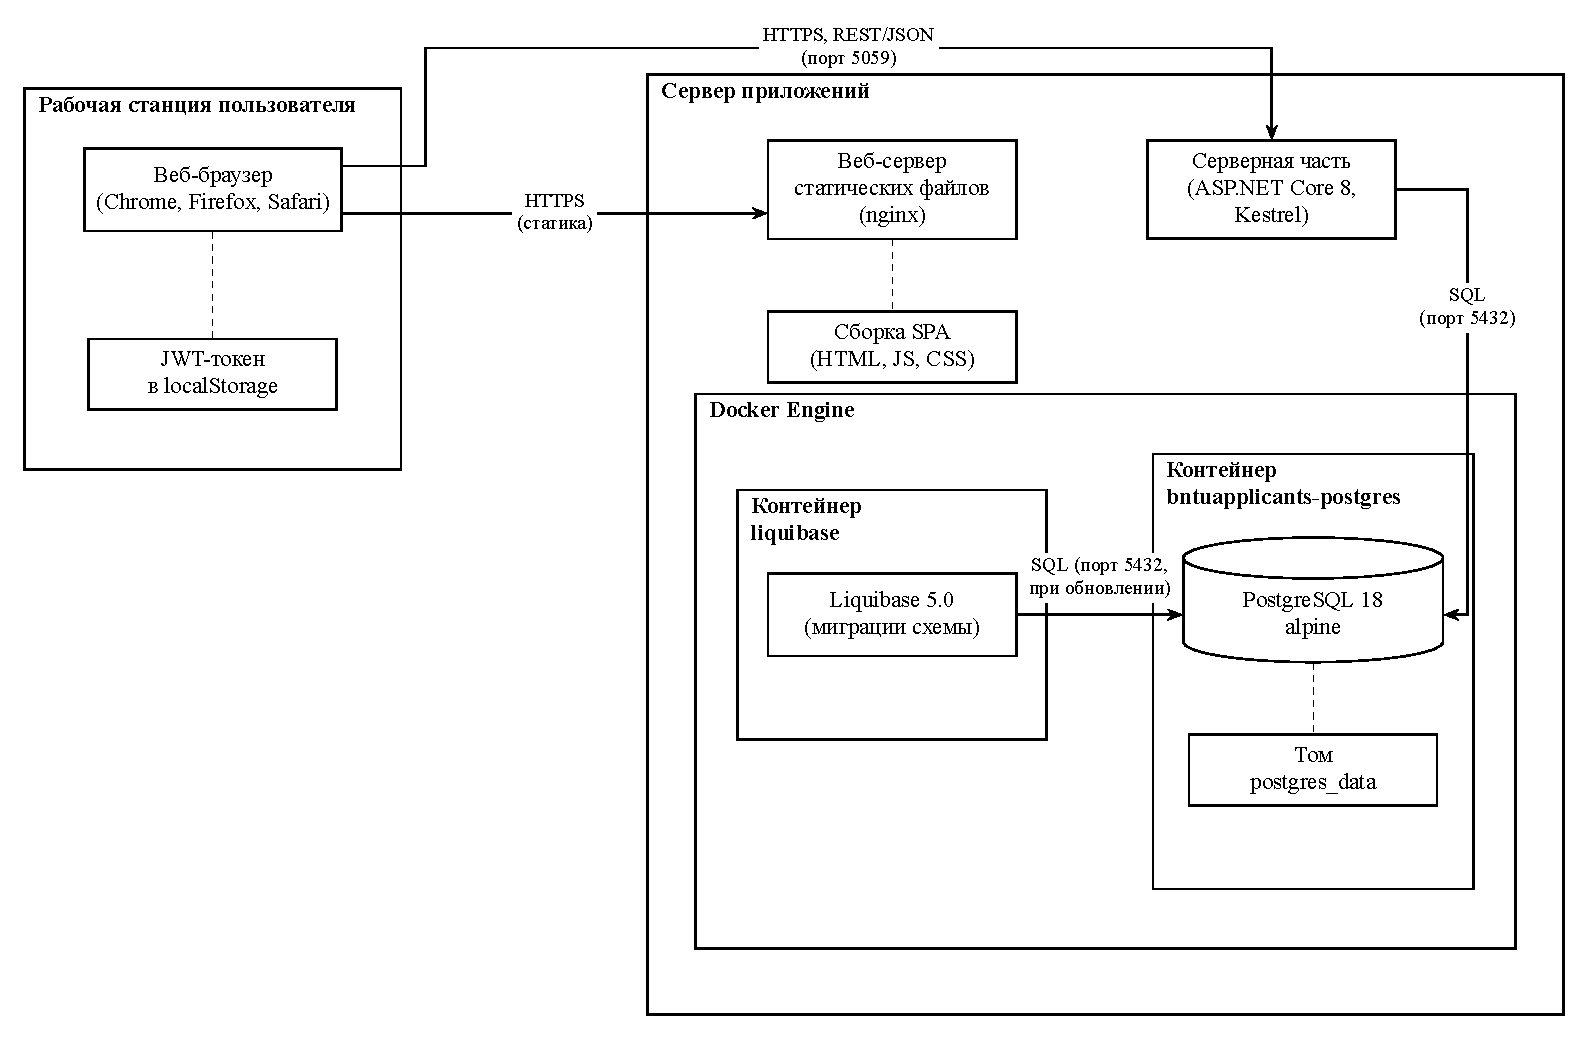
\includegraphics[width=\textwidth]{deployment}
\caption{Диаграмма развёртывания системы}
\label{fig:deployment}
\end{figure}

В составе развёртывания выделены два узла: рабочая станция пользователя и сервер приложений.

На рабочей станции пользователя выполняется только веб-браузер (поддерживаются последние версии Chrome, Firefox и Safari).
Браузер исполняет загруженную сборку клиентского одностраничного приложения и хранит JWT-токен доступа в локальном хранилище \code{localStorage}.
Установка какого-либо прикладного программного обеспечения на рабочую станцию не требуется, что упрощает развёртывание системы среди сотрудников приёмной комиссии.

Сервер приложений объединяет четыре программных компонента: веб-сервер статических файлов \code{nginx} (отдаёт сборку клиентского одностраничного приложения), серверную часть на платформе ASP.NET~Core с встроенным веб-сервером Kestrel (порт 5059), контейнер PostgreSQL 18 (порт 5432) и одноразовый контейнер Liquibase, применяющий миграции схемы при обновлении системы.
PostgreSQL и Liquibase развёртываются в Docker через отдельные файлы \code{infra/docker-compose.yml} и \code{liquibase/docker-compose.yml}.
Данные базы хранятся в именованном томе Docker \code{postgres\_data}, что обеспечивает их сохранность при пересоздании контейнера PostgreSQL.

Взаимодействие компонентов на сервере организовано следующим образом.
Веб-браузер пользователя обращается к веб-серверу статических файлов по протоколу HTTPS для загрузки сборки клиентского приложения, а затем к серверной части по REST API в формате JSON по протоколу HTTPS на порту~5059.
Серверная часть подключается к контейнеру PostgreSQL по протоколу TCP на порту~5432 через драйвер Npgsql.
Контейнер Liquibase подключается к тому же экземпляру PostgreSQL и выполняется однократно при запуске или обновлении системы~--~после применения недостающих миграций контейнер завершает работу.

Параметры подключения к базе данных (имя пользователя, пароль, имя базы, порт) задаются через файл переменных окружения \code{.env}, отдельный для каждого окружения (разработка, тестирование, эксплуатация).
Учётная запись администратора системы создаётся автоматически при первом запуске серверной части, если в таблице \code{users} нет ни одного пользователя; имя пользователя и пароль задаются переменными окружения \code{InitialAdmin\_\_Username} и \code{InitialAdmin\_\_Password} (значения по умолчанию~--~\code{admin} и \code{Admin@123}).

Сценарий обновления версии системы состоит из трёх шагов: остановки контейнера серверной части, запуска контейнера Liquibase для применения новых миграций схемы (контейнер завершается автоматически после успешного применения), запуска контейнера серверной части новой версии.
Контейнер PostgreSQL и его том данных при обновлении не пересоздаются, что обеспечивает сохранность данных приёмной кампании между версиями системы.
В случае отката версии порядок обратный, но в качестве дополнительной меры предосторожности необходимо создание резервной копии тома \code{postgres\_data} до применения миграций, поскольку не все миграции схемы обратимы.

Полные тексты конфигурационных файлов \code{docker-compose.yml} для PostgreSQL и Liquibase, \code{Dockerfile} контейнера Liquibase, шаблонов переменных окружения \code{.env.example} и пример SQL-миграции схемы приведены в приложении~А.

\subsection{Интернационализация интерфейса}

Поддержка двух языков интерфейса реализована на двух уровнях.

На клиентской части используется библиотека react-i18next с автоматическим определением языка через библиотеку i18next-browser-languagedetector.
Переключение языка осуществляется через компонент \code{Segmented} библиотеки Ant Design в заголовке страницы.
При смене языка интерфейс автоматически перерисовывается без перезагрузки страницы.
Локаль библиотеки Ant Design также переключается динамически между \code{ruRU} и \code{enUS} в файле \code{src/providers/GlobalProvider.jsx}.

На серверной части используется встроенный в платформу~.NET механизм \code{Microsoft.Extensions.Localization}.
Файлы ресурсов \code{SharedResources.ru.resx} и \code{SharedResources.en.resx} содержат переводы сообщений об ошибках.
Сообщения подключаются в контроллерах через инжектируемый интерфейс \code{IStringLocalizer<SharedResources>}.
Атрибуты валидации DTO используют ключи ресурсов в свойстве \code{ErrorMessage}, которые автоматически разрешаются через ту же систему ресурсов благодаря настройке \code{DataAnnotationsLocalization} в \code{Program.cs}.

Выбор языка ответа сервера выполняется на основе заголовка \code{Accept-Language}, передаваемого клиентом в каждом запросе.
По умолчанию используется русский язык.
        % 4 ПРОГРАММНАЯ РЕАЛИЗАЦИЯ
\section{Руководство пользователя}

\subsection{Вход в систему}

Доступ к приложению осуществляется через веб-браузер по адресу, заданному при развёртывании системы.
При первом обращении пользователь перенаправляется на страницу входа, на которой расположены поля ввода имени пользователя и пароля, переключатель языка интерфейса (русский или английский) и кнопка <<Войти>>.
Внешний вид страницы входа представлен на рисунке~\ref{fig:login}.

\begin{figure}[htbp]
\centering
\figureorstub{login}{скриншот страницы входа}
\caption{Страница входа в систему}
\label{fig:login}
\end{figure}

При успешной аутентификации пользователь перенаправляется на главную страницу приложения~--~страницу результатов отбора.
При неверных учётных данных на странице отображается сообщение об ошибке; каждая попытка входа фиксируется в журнале авторизации независимо от её исхода.
Форма проверяет заполненность обоих полей на стороне клиента: при попытке отправить пустую форму поля подсвечиваются с подсказкой об обязательности заполнения, а запрос на сервер не отправляется.
Переключатель языка над формой позволяет выбрать язык интерфейса до входа в систему; выбор сохраняется в локальном хранилище браузера и применяется автоматически при последующих сеансах.
Выбранный язык влияет не только на отображение текстов клиентской части: в заголовок каждого HTTP-запроса подставляется значение \code{Accept-Language}, благодаря чему сообщения об ошибках с сервера также возвращаются на выбранном языке.
После входа в систему пользователь может в любой момент сменить пароль через меню учётной записи в верхней части экрана.

\subsection{Главное меню и навигация}

Главное меню расположено в левой боковой панели приложения и содержит следующие пункты: <<Результаты>>, <<Абитуриенты>>, <<Факультеты>>, <<Кафедры>>, <<Специальности>>, <<Критерии оценивания>>, <<Группы критериев>>, <<Аудит>>, <<Журнал аудита>>, <<Пользователи>>.
Видимость пунктов меню одинакова для всех аутентифицированных пользователей; ограничения по ролям применяются на уровне конкретных операций (создание, изменение, удаление).
Внешний вид главного меню можно наблюдать в левой боковой панели на рисунке~\ref{fig:faculties}.

В верхней части каждой страницы расположен заголовок с переключателем темы (светлая или тёмная), переключателем языка интерфейса (русский или английский) и меню текущего пользователя.
Меню пользователя содержит пункты <<Сменить пароль>> и <<Выход>>.
Пункт <<Сменить пароль>> открывает диалоговое окно смены пароля, в котором необходимо ввести текущий пароль, новый пароль и его повтор.
Пункт <<Выход>> удаляет токен доступа из локального хранилища браузера и возвращает пользователя на страницу входа.

Переключение языка интерфейса применяется немедленно без перезагрузки страницы.
Одновременно с переводом текстов клиентской части в заголовок \code{Accept-Language} последующих HTTP-запросов подставляется выбранный язык, благодаря чему сервер возвращает сообщения об ошибках на том же языке.

\subsection{Работа со структурой университета}

Страницы <<Факультеты>>, <<Кафедры>> и <<Специальности>> построены по единому шаблону: таблица с серверной пагинацией и фильтрами в верхней части, кнопка <<Добавить>> над таблицей и кнопки <<Изменить>>, <<Удалить>> в каждой строке.
Кнопки записи отображаются только пользователям с правом \code{WriteStructure} (роли \code{SuperAdmin} и \code{DataAdministrator}).
Внешний вид страницы факультетов представлен на рисунке~\ref{fig:faculties}.

\begin{figure}[htbp]
\centering
\figureorstub{faculties}{скриншот страницы факультетов}
\caption{Страница факультетов}
\label{fig:faculties}
\end{figure}

Для добавления факультета пользователь нажимает кнопку <<Добавить>>, заполняет поля наименования и сокращённого наименования и подтверждает создание.
Аналогично создаются кафедры (с обязательным указанием факультета) и специальности (с указанием кафедры).
При попытке удалить факультет с привязанными кафедрами или кафедру с привязанными специальностями отображается сообщение об ошибке~--~целостность ссылок гарантируется внешними ключами на уровне базы данных.

Страница редактирования специальности содержит дополнительные вкладки с привязанными к специальности конкурсными списками и категориями приёма.
Для каждого конкурсного списка указывается его наименование (например, <<Бюджет>>, <<Платное>>) и общий план приёма.
В пределах конкурсного списка администратор формирует категории приёма: для каждой категории указывает её наименование, квоту мест, приоритет и группу критериев оценивания.
Внешний вид страницы редактирования специальности представлен на рисунке~\ref{fig:specialtyedit}.

\begin{figure}[htbp]
\centering
\figureorstub{specialty-edit}{скриншот страницы редактирования специальности}
\caption{Страница редактирования специальности}
\label{fig:specialtyedit}
\end{figure}

\subsection{Работа с критериями оценивания}

Страница <<Критерии оценивания>> содержит перечень всех показателей, по которым оцениваются абитуриенты.
Для каждого критерия указывается наименование, диапазон допустимых значений (поля \code{minvalue} и \code{maxvalue}) и тип: <<больше~--~лучше>> (\code{higher\_is\_better}) или <<меньше~--~лучше>> (\code{lower\_is\_better}).
Внешний вид страницы критериев оценивания представлен на рисунке~\ref{fig:criteria}.

\begin{figure}[htbp]
\centering
\figureorstub{evaluation-criteria}{скриншот страницы критериев оценивания}
\caption{Страница критериев оценивания}
\label{fig:criteria}
\end{figure}

Страница <<Группы критериев>> позволяет объединять критерии в именованные наборы, привязываемые впоследствии к категориям приёма.
В составе группы каждый критерий получает значение поля \code{priority}, определяющего порядок лексикографической сортировки кандидатов: критерий с меньшим значением \code{priority} учитывается в сравнении первым.
Внешний вид страницы редактирования группы критериев представлен на рисунке~\ref{fig:criteriagroup}.

\begin{figure}[htbp]
\centering
\figureorstub{evaluation-criteria-group-edit}{скриншот страницы редактирования группы критериев}
\caption{Страница редактирования группы критериев}
\label{fig:criteriagroup}
\end{figure}

\subsection{Работа с абитуриентами}

Страница <<Абитуриенты>> содержит таблицу всех зарегистрированных абитуриентов с возможностью фильтрации по имени, внешнему идентификатору документа и статусу валидации.
Внешний вид страницы представлен на рисунке~\ref{fig:applicants}.

\begin{figure}[htbp]
\centering
\figureorstub{applicants}{скриншот страницы списка абитуриентов}
\caption{Страница списка абитуриентов}
\label{fig:applicants}
\end{figure}

Для добавления нового абитуриента пользователь с правом \code{WriteApplicants} нажимает кнопку <<Добавить>> и заполняет форму: имя, внешний идентификатор документа, текстовые заметки.
Если в системе уже существует активная или удалённая запись с тем же внешним идентификатором, отображается сообщение об ошибке~--~уникальность внешнего идентификатора обеспечивается ограничением базы данных.

После сохранения абитуриента открывается страница его редактирования, на которой расположены вкладки для ввода оценок по критериям и для управления заявками в категории приёма.
Внешний вид страницы редактирования абитуриента представлен на рисунке~\ref{fig:applicantedit}.

\begin{figure}[htbp]
\centering
\figureorstub{applicant-edit}{скриншот страницы редактирования абитуриента}
\caption{Страница редактирования абитуриента}
\label{fig:applicantedit}
\end{figure}

На вкладке оценок отображается список всех критериев, доступных в системе.
Для каждого критерия пользователь вводит численное значение, которое автоматически проверяется на принадлежность диапазону, заданному для критерия.
При вводе значения вне диапазона выводится сообщение об ошибке с указанием границ.
При сохранении формы выполняется отправка изменений на сервер, после чего автоматически запускается пересчёт результатов отбора.

На вкладке заявок пользователь добавляет записи о подаче заявления в конкретные категории приёма с указанием приоритета предпочтения.
Один абитуриент может подать заявки в несколько категорий разных специальностей.
Поле приоритета предпочтения принимает целые положительные значения; меньшее значение соответствует более предпочтительной для абитуриента категории.

Удаление абитуриента выполняется в два этапа.
При нажатии кнопки <<Удалить>> в строке абитуриента создаётся запрос на удаление со статусом \code{pending}; абитуриент немедленно скрывается из всех таблиц и из результатов отбора, но физически из базы данных не удаляется.
Окончательное удаление либо отмена запроса выполняются на странице <<Аудит>> пользователем с правом \code{WriteAudit}.

\subsection{Просмотр результатов отбора}

Страница <<Результаты>> содержит список всех конкурсных списков системы с указанием специальности, общего плана приёма и количества зачисленных абитуриентов.
Внешний вид страницы представлен на рисунке~\ref{fig:results}.

\begin{figure}[htbp]
\centering
\figureorstub{results}{скриншот страницы результатов отбора}
\caption{Список результатов отбора}
\label{fig:results}
\end{figure}

Для каждой строки списка доступно скачивание результатов соответствующего конкурсного списка в формате Excel через ссылку <<Скачать Excel>>.
Сформированный файл содержит несколько листов~--~один лист на категорию приёма~--~и включает столбцы с именем абитуриента, внешним идентификатором документа, приоритетом предпочтения заявки и значениями всех критериев из группы категории.
Имя файла формируется автоматически на основе наименования специальности и конкурсного списка.

При выборе конкретного конкурсного списка открывается страница детального просмотра с разбиением по категориям.
Для каждой категории отображается её квота, приоритет защиты и список зачисленных абитуриентов с их оценками по критериям.
Внешний вид страницы детального просмотра представлен на рисунке~\ref{fig:competitionresult}.

\begin{figure}[htbp]
\centering
\figureorstub{competition-list-result}{скриншот страницы детального просмотра результатов конкурсного списка}
\caption{Детальный просмотр результатов конкурсного списка}
\label{fig:competitionresult}
\end{figure}

Кнопка <<Пересчитать>> над списком конкурсных списков позволяет вручную запустить пересчёт результатов отбора.
Кнопка доступна пользователям с правом \code{WriteStructure}.
В штатном режиме ручной запуск не требуется: пересчёт выполняется автоматически при каждом изменении данных абитуриентов, их оценок, заявок и при изменении состава критериев в группах.
Ручной запуск используется в случае разовых административных изменений данных непосредственно в базе данных в обход интерфейса, а также для пересчёта по запросу при отладке.

\subsection{Подсистема аудита}

Страница <<Аудит>> содержит пять вкладок, каждая из которых отображает один из видов оповещений системы.
Последовательно просматривая вкладки, оператор получает полную картину состояния данных, требующих проверки или обработки.
Внешний вид страницы аудита представлен на рисунке~\ref{fig:audit}.

\begin{figure}[htbp]
\centering
\figureorstub{audit}{скриншот страницы аудита}
\caption{Страница аудита}
\label{fig:audit}
\end{figure}

Вкладка <<Невалидированные абитуриенты>> отображает список абитуриентов, статус валидации которых равен \code{false}.
Пользователь с правом \code{WriteAudit} может подтвердить валидацию (\code{validated = true}) или вновь снять её для каждого абитуриента.
При последующем изменении любого поля данных абитуриента (имени, внешнего идентификатора, оценок, заявок) статус автоматически возвращается в значение \code{false}, и абитуриент вновь появляется в этой вкладке.

Вкладка <<Неполные данные>> отображает абитуриентов, у которых не заполнены оценки по всем критериям, требуемым категориями, в которые они подали заявки.
Для каждого такого абитуриента показывается список отсутствующих критериев~--~это позволяет оператору быстро устранить пробелы в данных.

Вкладка <<Некорректные группы критериев>> отображает группы критериев, в которых отсутствуют обязательные элементы или указаны неверные приоритеты.

Вкладка <<Некорректные конкурсные списки>> отображает конкурсные списки, в которых обнаружены проблемы с категориями приёма: отсутствие группы критериев, недопустимые значения квот или приоритетов.

Вкладка <<Запросы на удаление>> отображает запросы со статусом \code{pending}.
Для каждого запроса доступны кнопки <<Подтвердить>> и <<Отклонить>>.
При подтверждении абитуриент скрывается окончательно; при отклонении абитуриент возвращается в активные данные, помечается как невалидированный и автоматически запускается пересчёт результатов отбора.
После отклонения возможно создание нового запроса на удаление того же абитуриента.
Внешний вид вкладки запросов на удаление представлен на рисунке~\ref{fig:pendingdeletions}.

\begin{figure}[htbp]
\centering
\figureorstub{pending-deletions}{скриншот вкладки запросов на удаление}
\caption{Вкладка запросов на удаление страницы аудита}
\label{fig:pendingdeletions}
\end{figure}

Страница <<Журнал аудита>> отображает полный журнал всех действий пользователей с возможностью фильтрации по дате, действию, типу сущности и пользователю.
Внешний вид страницы журнала аудита представлен на рисунке~\ref{fig:auditlog}.

\begin{figure}[htbp]
\centering
\figureorstub{audit-log}{скриншот страницы журнала аудита}
\caption{Страница журнала аудита}
\label{fig:auditlog}
\end{figure}

В отдельной вкладке доступен журнал попыток входа в систему с указанием пользователя, времени, исхода и сетевого адреса источника попытки.
Внешний вид вкладки журнала входов представлен на рисунке~\ref{fig:authlog}.

\begin{figure}[htbp]
\centering
\figureorstub{auth-log}{скриншот вкладки журнала входов в систему}
\caption{Вкладка журнала входов в систему}
\label{fig:authlog}
\end{figure}

Для просмотра истории изменений конкретной сущности на странице её редактирования предусмотрена ссылка <<История изменений>>, открывающая отфильтрованный по идентификатору сущности журнал.
В записях вида \code{update} отображается разница состояний до и после изменения, что позволяет восстановить любое предыдущее состояние сущности.
Внешний вид окна истории изменений сущности представлен на рисунке~\ref{fig:entityhistory}.

\begin{figure}[htbp]
\centering
\figureorstub{entity-history}{скриншот окна истории изменений сущности}
\caption{Окно истории изменений сущности}
\label{fig:entityhistory}
\end{figure}

\subsection{Управление учётными записями пользователей}

Страница <<Пользователи>> доступна всем аутентифицированным пользователям для просмотра, но операции создания, изменения, активации и удаления учётных записей доступны только пользователю с ролью \code{SuperAdmin}.
Внешний вид страницы пользователей представлен на рисунке~\ref{fig:users}.

\begin{figure}[htbp]
\centering
\figureorstub{users}{скриншот страницы пользователей}
\caption{Страница управления учётными записями пользователей}
\label{fig:users}
\end{figure}

Создание учётной записи выполняется через кнопку <<Добавить>>: указываются имя пользователя, начальный пароль и роль из числа предусмотренных в системе.

В строке каждой учётной записи доступны кнопки изменения, переключения признака активности и удаления.
Деактивированная учётная запись сохраняется в базе данных, но не может войти в систему.
Удаление активного пользователя с ролью \code{SuperAdmin} разрешено только при условии, что в системе остаётся хотя бы один другой активный пользователь с этой ролью~--~это исключает возможность случайной потери единственной учётной записи с правами управления пользователями.
        % 5 РУКОВОДСТВО ПОЛЬЗОВАТЕЛЯ
\section{Тестирование приложения}

\subsection{Подход к тестированию}

Функциональное тестирование разработанного приложения проведено в соответствии с рекомендациями методички (раздел~4.2) и разделено на критическое и углубленное.
Критическое тестирование охватывает основные сценарии работы пользователя при корректных входных данных; углубленное~--~поведение системы при некорректных, граничных и пограничных значениях.

В рамках проекта применены два метода функционального тестирования: метод <<чёрного ящика>> для проверки эндпоинтов REST API через инструмент Swagger UI и метод <<белого ящика>> для проверки логики алгоритма пересчёта результатов отбора через юнит-тесты класса \code{FullRecalculationCore}.

\subsection{Перечень аппаратных средств}

Аппаратные средства, использованные при тестировании, приведены в таблице~\ref{tab:hardware}.

\begin{longtblr}[
  caption = {Перечень аппаратных средств},
  label = {tab:hardware},
]{
  colspec = {|Q[c]|Q[l]|X|X|},
  width = \textwidth,
  hlines, vlines,
  rowhead = 1,
  row{1} = {halign=c},
}
№ & Роль & Аппаратная конфигурация & Программная конфигурация \\
1 & Сервер приложений & Apple M1, 16~ГБ ОЗУ & macOS 25, .NET 8 SDK, Docker \\
2 & Сервер базы данных & Тот же компьютер & PostgreSQL 18-alpine в контейнере Docker \\
3 & Рабочая станция & Apple M1, 16~ГБ ОЗУ & macOS 25, браузер Chrome 138 \\
\end{longtblr}

\subsection{Результаты функционального тестирования API}

Тестовые случаи для проверки эндпоинтов REST API и результаты их прохождения приведены в таблице~\ref{tab:apitests}.

\begin{longtblr}[
  caption = {Тестовые случаи для проверки REST API},
  label = {tab:apitests},
]{
  colspec = {|Q[c]|X|X|X|Q[c]|},
  width = \textwidth,
  hlines, vlines,
  rowhead = 1,
  row{1} = {halign=c},
}
№ & Название модуля & Описание тестового случая & Ожидаемый результат & Пройден? \\
1 & Аутентификация & POST \code{/auth/login} с корректными учётными данными & Возвращён JWT-токен, статус~200 & Да \\
2 & Аутентификация & POST \code{/auth/login} с неверным паролем & Статус~401, в \code{auth\_log} запись с неуспехом & Да \\
3 & Факультеты & POST \code{/faculties} от пользователя с ролью \code{SuperAdmin} & Факультет создан, статус~200 & Да \\
4 & Факультеты & POST \code{/faculties} от пользователя с ролью \code{DataViewer} & Статус~403 (Forbidden) & Да \\
5 & Факультеты & GET \code{/faculties/paged?page=1\&pageSize=10} & Возвращены первые 10 факультетов & Да \\
6 & Абитуриенты & POST \code{/applicants} с корректными данными & Абитуриент создан, статус~200 & Да \\
7 & Абитуриенты & DELETE \code{/applicants/\{id\}} & Создан запрос на удаление со статусом \code{pending}, абитуриент исключён из списков & Да \\
8 & Оценки & POST \code{/applicant\_evaluation\_values} со значением вне диапазона критерия & Статус~400, сообщение об ошибке & Да \\
9 & Оценки & POST дублирующего значения по той же паре (абитуриент, критерий) & Статус~409 (Conflict) благодаря уникальному ограничению & Да \\
10 & Отбор & POST \code{/selection/recalculate} & Таблица \code{selectedapplicants} перестроена & Да \\
11 & Отбор & GET \code{/selection/competition-lists/\{id\}/excel} & Возвращён файл \code{xlsx} с заголовком \code{Content-Disposition} & Да \\
12 & Аудит & POST \code{/audit/pending-deletions/\{id\}/confirm} & Запрос помечен \code{confirmed}, абитуриент скрыт окончательно & Да \\
13 & Аудит & POST \code{/audit/pending-deletions/\{id\}/reject} & Абитуриент возвращён, \code{validated=false}, выполнен пересчёт & Да \\
\end{longtblr}

\subsection{Тестирование алгоритма отбора}

Для проверки корректности работы алгоритма пересчёта результатов отбора разработан набор юнит-тестов, проверяющих следующие сценарии: распределение абитуриентов в одну категорию без вытеснения; вытеснение слабого кандидата при превышении квоты категории; вытеснение слабого кандидата при превышении общего плана конкурсного списка; корректную обработку нескольких заявок одного абитуриента в порядке приоритета предпочтения; работу с критериями типа \code{lower\_is\_better}; обработку категорий с пустой группой критериев.

Все разработанные тестовые случаи пройдены успешно, что подтверждает корректность реализации алгоритма.

\subsection{Перечень граничных и эквивалентных значений}

В соответствии с рекомендациями методички (раздел~4.2.2.6) для полей с числовыми значениями определены граничные и эквивалентные классы значений.
Результаты приведены в таблице~\ref{tab:boundary}.

\begin{longtblr}[
  caption = {Перечень граничных и эквивалентных значений},
  label = {tab:boundary},
]{
  colspec = {|X|X|X|X|},
  width = \textwidth,
  hlines, vlines,
  rowhead = 1,
  row{1} = {halign=c},
}
Название поля & Формат данных & Граничные значения & Эквивалентные значения \\
Значение оценки & \code{decimal} с двумя знаками после запятой & \code{minvalue}, \code{maxvalue} & \code{minvalue - 0.01}, среднее значение диапазона, \code{maxvalue + 0.01} \\
Квота категории & \code{integer} & 0, 1 & --10, 100 \\
План конкурсного списка & \code{integer} & 0, 1 & 100 \\
Приоритет защиты & \code{integer} & 1 & 2, 99 \\
Приоритет предпочтения & \code{integer} & 1 & 2, 100 \\
\end{longtblr}

\subsection{Выводы по тестированию}

По результатам функционального тестирования установлено, что разработанное приложение корректно реализует все сформулированные функциональные требования.
Все запланированные тестовые случаи (13 шт.) пройдены успешно.
Обнаруженные в процессе разработки ошибки были устранены до этапа итогового тестирования.

Алгоритм пересчёта результатов отбора, реализованный в классе \code{FullRecalculationCore}, продемонстрировал корректность работы на всех проверенных сценариях, включая граничные случаи с превышением квот и плана конкурсного списка.
        % 6 ТЕСТИРОВАНИЕ ПРИЛОЖЕНИЯ
% Локальный макрос: кириллическая переменная в math-режиме.
% Math-режим в XeLaTeX берёт глифы из math-шрифта, в котором кириллицы нет;
% \rv{...} оборачивает символ в \text{}, что использует основной текстовый
% шрифт (Times New Roman) и корректно отображает русские буквы.
\providecommand{\rv}[1]{\text{#1}}

\section{Экономическое обоснование проекта по разработке программного обеспечения}

Цель настоящего раздела~--~подтвердить экономическую целесообразность разработки и применения системы компьютеризации ввода и мониторинга информации об абитуриентах при поступлении в БНТУ.
Раздел охватывает четыре содержательных вопроса: описание функций, назначения и потенциальных пользователей программного продукта, расчёт затрат на разработку, оценку экономического эффекта от внедрения и расчёт показателей эффективности инвестиций.

\subsection{Описание функций, назначения и потенциальных пользователей программного обеспечения}

Разработанное программное обеспечение представляет собой веб-приложение для автоматизации работы приёмной комиссии Белорусского национального технического университета.
Программный продукт предназначен для замены применяемых в настоящее время разрозненных средств учёта (электронных таблиц с макросами, локальных баз данных, ручного пересчёта рейтингов) единой централизованной информационной системой.

Основными функциями программного обеспечения являются:
\begin{itemize}
\item ведение организационной структуры университета~--~факультетов, кафедр, специальностей~--~через интерфейс администратора;
\item ведение конкурсных списков и категорий приёма с настраиваемыми планами, квотами и приоритетами защиты;
\item ведение справочника показателей оценивания абитуриентов и групп критериев с настраиваемыми правилами ранжирования;
\item ввод данных абитуриентов и их заявок в категории приёма;
\item автоматический пересчёт результатов отбора при любом изменении данных абитуриентов;
\item валидация введённых данных силами второго оператора по принципу двойного контроля;
\item ведение журнала действий пользователей (аудит) и журнала авторизации;
\item двухступенчатое удаление абитуриентов (soft-delete) с возможностью отката;
\item выгрузка результатов отбора в формате Excel для последующей обработки.
\end{itemize}

Потенциальными пользователями системы являются:
\begin{itemize}
\item сотрудники приёмной комиссии БНТУ, ответственные за ввод и обработку данных абитуриентов;
\item сотрудники приёмной комиссии БНТУ, выполняющие функции аудиторов и подтверждающие корректность введённых данных;
\item ответственные сотрудники кафедр и факультетов, ведущие справочники структуры и конкурсных списков;
\item администраторы информационной системы БНТУ, выполняющие конфигурирование, управление учётными записями и сопровождение;
\item опосредованно~--~абитуриенты, получающие достоверные и оперативно публикуемые результаты конкурсного отбора.
\end{itemize}

Потребность в программном продукте обусловлена ежегодным масштабом приёмной кампании БНТУ: количество подаваемых заявлений составляет порядка пяти тысяч и более, при этом нормативная база приёма периодически меняется, а ручной пересчёт рейтингов с использованием электронных таблиц трудоёмок и подвержен ошибкам.
Внедрение системы позволит сократить трудоёмкость рутинных операций, повысить достоверность результатов отбора за счёт автоматического пересчёта и валидации, а также обеспечить полноту прослеживаемости действий пользователей и истории изменений сущностей.

Косвенно потенциальными пользователями являются другие учреждения высшего образования Республики Беларусь, использующие сходную модель конкурентного зачисления по приоритетам и нуждающиеся в инструменте, который не привязан к нормативной базе других государств и допускает изменение правил приёма через интерфейс администратора.

\subsection{Расчёт затрат на разработку программного обеспечения}

Затраты на разработку программного обеспечения определяются по статьям: основная заработная плата команды разработчиков; дополнительная заработная плата; отчисления на социальные нужды; прочие затраты.

\subsubsection{Затраты на основную заработную плату команды разработчиков}

Затраты на основную заработную плату определяются исходя из состава и численности команды разработчиков, размеров месячной заработной платы каждого участника и общей трудоёмкости разработки программного обеспечения и рассчитываются по формуле

\begin{equation}
\label{eq:zo}
\rv{З}_\rv{о} = \rv{К}_\rv{пр} \cdot \sum_{i=1}^{n} \rv{З}_{\rv{ч},i} \cdot t_i,
\end{equation}

\begin{explanationx}
\item где $\rv{К}_\rv{пр}$~--~коэффициент премии, принимаемый в диапазоне 1,5--2,0;
\item $\mathrm{n}$~--~количество исполнителей, занятых разработкой;
\item $\rv{З}_{\rv{ч},\mathrm{i}}$~--~часовая заработная плата $\mathrm{i}$-го исполнителя, руб.;
\item $\mathrm{t}_\mathrm{i}$~--~трудоёмкость работ, выполняемых $\mathrm{i}$-м исполнителем, ч.
\end{explanationx}

Часовая заработная плата $i$-го исполнителя определяется делением месячного оклада на среднемесячный фонд рабочего времени, принимаемый равным 168~ч.
Размеры месячной заработной платы приняты на уровне рыночных значений по данным портала rabota.by для города Минска по состоянию на 2026~г.
Коэффициент премии принят равным $\rv{К}_\rv{пр} = 1{,}5$.

Состав команды разработчиков, трудоёмкость работ и расчёт затрат на основную заработную плату приведены в таблице~\ref{tab:zo}.

\begin{longtblr}[
  caption = {Расчёт затрат на основную заработную плату команды разработчиков},
  label = {tab:zo},
]{
  colspec = {|X[0.4,c,m]|X[1.9,l,m]|X[2.4,l,m]|X[1,c,m]|X[1,c,m]|X[2.1,c,m]|X[1.2,c,m]|},
  cells = {font=\small, cmd={\sloppy}},
  leftsep = 2pt,
  rightsep = 2pt,
  width = \textwidth,
  hlines, vlines,
  rowhead = 1,
  row{1} = {halign=c},
}
№ & Участник команды & Вид выполняемой работы & Оклад, руб. & Ставка, руб./ч & Трудоёмкость, ч & З/п по тарифу, руб. \\
1 & Бизнес-аналитик & Анализ требований, проектирование доменной модели & 2400 & 14,29 & 60 & 857,40 \\
2 & Full-stack .NET-разработчик & Реализация серверной (ASP.NET Core, PostgreSQL) и клиентской (React) частей & 3500 & 20,83 & 480 & 9998,40 \\
3 & Тестировщик & Функциональное и регрессионное тестирование & 2400 & 14,29 & 120 & 1714,80 \\
\SetCell[c=6]{l} Итого по тарифу & & & & & & 12~570,60 \\
\SetCell[c=6]{l} Премия (50\%) & & & & & & 6285,30 \\
\SetCell[c=6]{l} Итого $\rv{З}_\rv{о}$ & & & & & & 18~855,90 \\
\end{longtblr}

\subsubsection{Затраты на дополнительную заработную плату команды разработчиков}

Дополнительная заработная плата включает выплаты, предусмотренные законодательством о труде (оплата трудовых отпусков, льготных часов, времени выполнения государственных обязанностей и других выплат, не связанных с основной деятельностью исполнителей), и определяется по формуле

\begin{equation}
\label{eq:zd}
\rv{З}_\rv{д} = \frac{\rv{З}_\rv{о} \cdot \rv{Н}_\rv{д}}{100},
\end{equation}

\begin{explanationx}
\item где $\rv{З}_\rv{о}$~--~затраты на основную заработную плату, руб.;
\item $\rv{Н}_\rv{д}$~--~норматив дополнительной заработной платы, \%.
\end{explanationx}

Норматив принимаем $\rv{Н}_\rv{д} = 15$~\%.
Тогда

\[
\rv{З}_\rv{д} = \frac{18\,855{,}90 \cdot 15}{100} \approx 2828{,}39 \text{ (руб.).}
\]

\subsubsection{Отчисления на социальные нужды}

Отчисления в Фонд социальной защиты населения и на обязательное страхование определяются в соответствии с действующими законодательными актами Республики Беларусь по формуле

\begin{equation}
\label{eq:rsoc}
\rv{Р}_\rv{соц} = \frac{(\rv{З}_\rv{о} + \rv{З}_\rv{д}) \cdot \rv{Н}_\rv{соц}}{100},
\end{equation}

\begin{explanationx}
\item где $\rv{Н}_\rv{соц}$~--~суммарный норматив отчислений на социальные нужды, \%.
\end{explanationx}

В соответствии с действующим законодательством Республики Беларусь принимаем $\rv{Н}_\rv{соц} = 34$~\%.
Тогда

\[
\rv{Р}_\rv{соц} = \frac{(18\,855{,}90 + 2828{,}39) \cdot 34}{100} \approx 7372{,}66 \text{ (руб.).}
\]

\subsubsection{Прочие затраты}

Прочие затраты (амортизационные отчисления, расходы на электроэнергию, аренду помещений и оборудования, расходы на управление) включаются в себестоимость разработки в процентах от затрат на основную заработную плату и определяются по формуле

\begin{equation}
\label{eq:zpz}
\rv{З}_\rv{пз} = \frac{\rv{З}_\rv{о} \cdot \rv{Н}_\rv{пз}}{100},
\end{equation}

\begin{explanationx}
\item где $\rv{Н}_\rv{пз}$~--~норматив прочих затрат, \%.
\end{explanationx}

Норматив принимаем $\rv{Н}_\rv{пз} = 100$~\%.
Тогда

\[
\rv{З}_\rv{пз} = \frac{18\,855{,}90 \cdot 100}{100} = 18\,855{,}90 \text{ (руб.).}
\]

Полная сумма затрат на разработку программного обеспечения находится суммированием всех рассчитанных статей затрат и приведена в таблице~\ref{tab:zr}.

\begin{longtblr}[
  caption = {Затраты на разработку программного обеспечения},
  label = {tab:zr},
]{
  colspec = {|X[l,m]|X[1,c,m]|},
  width = \textwidth,
  hlines, vlines,
  rowhead = 1,
  row{1} = {halign=c},
}
Статья затрат & Сумма, руб. \\
Основная заработная плата команды разработчиков & 18~855,90 \\
Дополнительная заработная плата команды разработчиков & 2828,39 \\
Отчисления на социальные нужды & 7372,66 \\
Прочие затраты & 18~855,90 \\
Общая сумма затрат на разработку $\rv{З}_\rv{р}$ & 47~912,85 \\
\end{longtblr}

Таким образом, общая сумма затрат на разработку программного обеспечения составляет 47~912,85~руб.

\subsection{Оценка экономического эффекта от внедрения программного обеспечения}

Разрабатываемое программное обеспечение предназначено для удовлетворения собственных потребностей БНТУ как государственного учреждения высшего образования и не предполагает свободной реализации на рынке.
В связи с этим экономический эффект от его применения состоит в экономии трудозатрат при выполнении операций приёмной кампании.

Источники экономии трудозатрат и их оценочные значения приведены в таблице~\ref{tab:savings}.
Часовая ставка оператора приёмной комиссии БНТУ принята равной 12~руб./ч.

\begin{longtblr}[
  caption = {Оценка экономии трудозатрат при внедрении системы},
  label = {tab:savings},
]{
  colspec = {|X[l,m]|X[1,c,m]|X[1,c,m]|},
  width = \textwidth,
  hlines, vlines,
  rowhead = 1,
  row{1} = {halign=c},
}
Операция & Экономия времени, ч/год & Экономия, руб./год \\
Ввод данных абитуриентов в структурированные формы (5000~заявлений по 10~мин) & 833 & 9996 \\
Кросс-проверка и валидация введённых данных (5000~заявлений по 3~мин) & 250 & 3000 \\
Автоматический пересчёт результатов отбора после изменений (50~пересчётов по 4~ч) & 200 & 2400 \\
Автоматическая выгрузка отчётов в Excel (30~выгрузок по 2~ч) & 60 & 720 \\
Снижение трудозатрат на исправление ошибок благодаря средствам аудита, валидации и soft-delete & 100 & 1200 \\
Итого экономия $\rv{Э}_\rv{з}$ & 1443 & 17~316 \\
\end{longtblr}

С учётом округления принимаем $\rv{Э}_\rv{з} \approx 17\,300$~руб./год.

Прирост текущих затрат, связанных с эксплуатацией системы ($\Delta\rv{З}_\rv{тек}$), включает дополнительные расходы на электроэнергию и амортизацию серверной нагрузки (около 300~руб./год), а также сопровождение и мелкие доработки силами ИТ-отдела БНТУ (около 700~руб./год).
Итого $\Delta\rv{З}_\rv{тек} \approx 1000$~руб./год.

Прирост чистой прибыли от внедрения программного обеспечения для собственных нужд определяется по формуле

\begin{equation}
\label{eq:dpch}
\Delta\rv{П}_\rv{ч} = (\rv{Э}_\rv{з} - \Delta\rv{З}_\rv{тек}) \cdot (1 - \rv{Н}_\rv{п}),
\end{equation}

\begin{explanationx}
\item где $\rv{Э}_\rv{з}$~--~экономия текущих затрат, полученная в результате применения программного обеспечения, руб.;
\item $\Delta\rv{З}_\rv{тек}$~--~прирост текущих затрат, связанных с эксплуатацией программного обеспечения, руб.;
\item $\rv{Н}_\rv{п}$~--~ставка налога на прибыль в соответствии с действующим законодательством Республики Беларусь, в долях единицы.
\end{explanationx}

Белорусский национальный технический университет как государственное учреждение высшего образования освобождён от уплаты налога на прибыль на доходы от основной деятельности (Налоговый кодекс Республики Беларусь, ст.~181) [\ref{src:laws:nalogkodex}], поэтому $\rv{Н}_\rv{п} = 0$.
Тогда

\[
\Delta\rv{П}_\rv{ч} = (17\,300 - 1000) \cdot (1 - 0) = 16\,300 \text{ (руб./год).}
\]

Полученный годовой экономический эффект составляет 16~300~руб./год.

\subsection{Расчёт показателей эффективности инвестиций в разработку программного обеспечения}

Затраты на разработку программного обеспечения $\rv{З}_\rv{р} = 47\,912{,}85$~руб. превышают годовой экономический эффект $\Delta\rv{П}_\rv{ч} = 16\,300$~руб./год, поэтому простая окупаемость составляет более одного года и экономическая целесообразность инвестиций оценивается на основе расчёта дисконтированных показателей: чистого дисконтированного дохода (ЧДД), срока окупаемости ($\rv{Т}_\rv{ок}$) и рентабельности инвестиций ($\rv{Р}_\rv{и}$).

Расчётный период принят равным четырём годам и включает один год разработки и три года эксплуатации программного обеспечения.

Поскольку экономический эффект и инвестиции относятся к разным годам расчётного периода, для обеспечения сопоставимости они приводятся к началу расчётного периода путём умножения на коэффициент дисконтирования соответствующего года~$t$, определяемый по формуле

\begin{equation}
\label{eq:alpha}
\alpha_t = \frac{1}{(1 + \rv{Е}_\rv{н})^t},
\end{equation}

\begin{explanationx}
\item где $\rv{Е}_\rv{н}$~--~норма дисконта, в долях единицы;
\item $\mathrm{t}$~--~порядковый номер года расчётного периода.
\end{explanationx}

Норма дисконта принимается на уровне ставки рефинансирования Национального банка Республики Беларусь, действующей на момент проведения расчётов, с добавлением двух процентных пунктов.
Ставка рефинансирования Национального банка Республики Беларусь, действующая с 19~марта 2025~г., составляет 9,5~\% [\ref{src:nbrb-rate}].
С учётом надбавки в два процентных пункта принимаем $\rv{Е}_\rv{н} = 11{,}5$~\%.

Чистый дисконтированный доход за расчётный период определяется по формуле

\begin{equation}
\label{eq:npv}
\rv{ЧДД} = \sum_{t=1}^{n} (\rv{Р}_t \cdot \alpha_t - \rv{З}_t \cdot \alpha_t),
\end{equation}

\begin{explanationx}
\item где $\mathrm{n}$~--~расчётный период, лет;
\item $\rv{Р}_\mathrm{t}$~--~результат (экономический эффект), полученный в году~$\mathrm{t}$, руб.;
\item $\rv{З}_\mathrm{t}$~--~затраты (инвестиции), осуществлённые в году~$\mathrm{t}$, руб.
\end{explanationx}

Рентабельность инвестиций рассчитывается как отношение суммы дисконтированных результатов к сумме дисконтированных инвестиций по формуле

\begin{equation}
\label{eq:pi}
\rv{Р}_\rv{и} = \frac{\sum_{t=1}^{n} \rv{Р}_t \cdot \alpha_t}{\sum_{t=1}^{n} \rv{З}_t \cdot \alpha_t}.
\end{equation}

Расчёт показателей эффективности инвестиционного проекта приведён в таблице~\ref{tab:npv}.

\begin{longtblr}[
  caption = {Расчёт эффективности инвестиционного проекта по разработке программного обеспечения},
  label = {tab:npv},
]{
  colspec = {|X[2,l,m]|X[1,c,m]|X[1,c,m]|X[1,c,m]|X[1,c,m]|},
  width = \textwidth,
  hlines, vlines,
  rowhead = 1,
  row{1} = {halign=c},
}
Показатель & 1~год & 2~год & 3~год & 4~год \\
Коэффициент дисконтирования $\alpha_t$ & 0,897 & 0,804 & 0,721 & 0,647 \\
Экономический эффект $\rv{Р}_t$, руб. & 16~300 & 16~300 & 16~300 & 16~300 \\
Дисконтированный результат $\rv{Р}_t \cdot \alpha_t$, руб. & 14~621 & 13~105 & 11~752 & 10~546 \\
Инвестиции $\rv{З}_t$, руб. & 47~913 & 0 & 0 & 0 \\
Дисконтированные инвестиции $\rv{З}_t \cdot \alpha_t$, руб. & 42~978 & 0 & 0 & 0 \\
ЧДД по годам, руб. & --28~357 & 13~105 & 11~752 & 10~546 \\
ЧДД нарастающим итогом, руб. & --28~357 & --15~252 & --3500 & 7046 \\
\end{longtblr}

По результатам расчёта получены следующие показатели эффективности инвестиционного проекта:
\begin{itemize}
\item чистый дисконтированный доход на конец расчётного периода составляет $\rv{ЧДД} = 7046$~руб., что больше нуля и подтверждает экономическую эффективность инвестиций;
\item срок окупаемости проекта находится между третьим и четвёртым годом расчётного периода и составляет ориентировочно $\rv{Т}_\rv{ок} \approx 3{,}33$~года;
\item рентабельность инвестиций составляет $\rv{Р}_\rv{и} = 50\,024 / 42\,978 \approx 1{,}164$, что больше единицы и также подтверждает экономическую целесообразность вложения средств в разработку.
\end{itemize}

Все три показателя согласованно подтверждают экономическую эффективность проекта.
При этом выполненный расчёт является консервативным: норма дисконта принята с надбавкой в два процентных пункта к ставке рефинансирования Национального банка Республики Беларусь, а в составе экономии текущих затрат учтены только прямые сокращения трудозатрат сотрудников приёмной комиссии; косвенные эффекты внедрения~--~снижение количества ошибок ручного ввода, сокращение времени получения промежуточных рейтингов абитуриентами, повышение прозрачности приёмной кампании~--~в денежной форме не оценивались.

Срок окупаемости 3,33~года формально превышает половину расчётного периода, однако согласуется со сроком эксплуатации программного обеспечения такого класса: типовой жизненный цикл системы поддержки приёмной кампании ограничен изменениями нормативной базы приёма (Правила приёма в учреждения высшего образования пересматриваются раз в три-пять лет [\ref{src:laws:admission}]) и связанной с ними доработкой алгоритмов отбора.

Чувствительность результата к исходным параметрам расчёта невысока: снижение годовой экономии трудозатрат на 10~\% уменьшает чистый дисконтированный доход примерно на пять тысяч рублей, но не делает его отрицательным, а индекс рентабельности инвестиций остаётся выше единицы.

Таким образом, разработка системы компьютеризации ввода и мониторинга информации об абитуриентах при поступлении в БНТУ является экономически целесообразной: за четырёхлетний горизонт планирования инвестиции в её разработку окупаются с положительным чистым дисконтированным доходом, а рентабельность инвестиций превышает единицу.
Полученный экономический эффект достигается за счёт автоматизации всех ключевых этапов приёмной кампании БНТУ~--~от ввода данных абитуриента и его заявок до публикации результатов конкурсного отбора.
        % 7 ЭКОНОМИЧЕСКОЕ ОБОСНОВАНИЕ
\providecommand{\rv}[1]{\text{#1}}

\section{Охрана труда}

\subsection{Производственная санитария, техника безопасности и пожарная профилактика}

Пользователи ПЭВМ могут подвергаться воздействию опасных и вредных производственных факторов, таких как повышенные уровни: электромагнитного, ультрафиолетового и инфракрасного излучения; статического электричества; повышенное или пониженное содержание аэроионов в воздухе рабочей зоны; повышенный или пониженный уровень освещённости рабочей зоны; содержание в воздухе рабочей зоны вредных веществ (оксид углерода, озон, аммиак, фенол, формальдегид); напряжение зрения, памяти, внимания; длительное статическое напряжение; монотонность труда; нерациональная организация рабочего места; эмоциональные перегрузки.

Требования к рабочим местам пользователей ПЭВМ приведены в Гигиеническом нормативе <<Показатели безопасности и безвредности факторов производственной среды и трудового процесса при работе с видеодисплейными терминалами и электронно-вычислительными машинами>> (постановление Совета Министров Республики Беларусь от 25.01.2021~г. №~37, в~ред. от 29.11.2022~г. №~829) [\ref{src:sanpin2}] и Типовой инструкцией по охране труда при использовании в работе офисного оборудования (постановление Министерства труда и социальной защиты от 14.04.2021~г. №~25) [\ref{src:office-instruction}].

Площадь помещения на одного пользователя ПЭВМ на базе плоских дискретных экранов (жидкокристаллических, плазменных) должна быть не менее 4{,}5~м\textsuperscript{2}.

\subsubsection{Метеоусловия}

В производственных помещениях, в которых работа с использованием ПЭВМ является основной (операторские, расчётные, посты управления, залы вычислительной техники), обеспечиваются оптимальные параметры микроклимата (таблица~\ref{tab:microclimate}).
Работа с компьютером относится к категории 1а (работы, производимые сидя и сопровождающиеся незначительным физическим напряжением, при которых расход энергии составляет до 120~ккал/ч, т.~е. до 139~Вт).

\begin{longtblr}[
  caption = {Оптимальные параметры микроклимата для помещений с ВДТ, ЭВМ и ПЭВМ},
  label = {tab:microclimate},
]{
  colspec = {|X[1,c,m]|X[1,c,m]|X[1.5,c,m]|X[1.5,c,m]|X[1.5,c,m]|},
  cells = {font=\small},
  width = \textwidth,
  hlines, vlines,
  rowhead = 1,
  row{1} = {halign=c},
}
Период года & Категория работ & Температура воздуха, \textdegree{}С, не более & Относительная влажность воздуха, \% & Скорость движения воздуха, м/с \\
Холодный & 1а & 22--24 & 40--60 & 0{,}1 \\
Тёплый & 1а & 23--25 & 40--60 & 0{,}1 \\
\end{longtblr}

Интенсивность теплового излучения работающих от нагретых поверхностей технологического оборудования, осветительных приборов, инсоляции на постоянных рабочих местах не превышает значений, указанных в таблице~\ref{tab:ir-radiation}.

\begin{longtblr}[
  caption = {Предельно допустимые уровни интенсивности излучения в инфракрасном и видимом диапазоне излучения на расстоянии 0{,}5~м со стороны экрана ВДТ, ЭВМ и ПЭВМ},
  label = {tab:ir-radiation},
]{
  colspec = {|X[1.4,l,m]|X[1,c,m]|X[1,c,m]|X[1,c,m]|},
  cells = {font=\small},
  width = \textwidth,
  hlines, vlines,
  rowhead = 1,
  row{1} = {halign=c},
}
Диапазоны длин волн & 400--760~нм & 760--1050~нм & свыше 1050~нм \\
Предельно допустимые уровни & 0{,}1~Вт/м\textsuperscript{2} & 0{,}05~Вт/м\textsuperscript{2} & 4{,}0~Вт/м\textsuperscript{2} \\
\end{longtblr}

Для создания нормальных метеорологических условий наиболее целесообразно уменьшить тепловыделения от самого источника~--~монитора, что предусматривается при разработке его конструкции.

В производственных помещениях для обеспечения необходимых показателей микроклимата предусмотрены системы отопления, вентиляции и кондиционирования воздуха.

\subsubsection{Вентиляция и отопление}

Воздух рабочей зоны помещения соответствует санитарно-гигиеническим требованиям по содержанию вредных веществ и частиц пыли, приведённым в ГОСТ~12.1.005--88 ССБТ <<Общие санитарно-гигиенические требования к воздуху рабочей зоны>> [\ref{src:gost-air}] и Гигиеническом нормативе <<Показатели безопасности и безвредности микроорганизмов продуцентов, микробных препаратов и их компонентов, вредных веществ в воздухе рабочей зоны и на кожных покровах работающих>> (постановление Совета Министров Республики Беларусь от 25.01.2021~г. №~37) [\ref{src:sanpin2}].

В помещениях проводится ежедневная влажная уборка и проветривание после каждого часа работы.

Уровни положительных и отрицательных аэроионов, а также коэффициент униполярности в воздухе всех помещений, где расположены ПЭВМ, соответствуют значениям, указанным в таблице~\ref{tab:aeroions}.

\begin{longtblr}[
  caption = {Аэроионный состав воздуха в зоне дыхания производственных и общественных помещений},
  label = {tab:aeroions},
]{
  colspec = {|X[1.3,l,m]|X[1.6,c,m]|X[1.1,c,m]|},
  cells = {font=\small},
  width = \textwidth,
  hlines, vlines,
  rowhead = 1,
  row{1} = {halign=c},
}
Уровни аэроионизации & Концентрация аэроионов, $\rho$ (ион/см\textsuperscript{3}) & Коэффициент униполярности, У \\
Минимально допустимые & $\rho\,\text{<<+>>} \geq 400 \quad \rho\,\text{<<--{}>>} \geq 600$ & \SetCell[r=2]{c,m} $0{,}4 < \rv{У} < 1{,}0$ \\
Максимально допустимые & $\rho\,\text{<<+>>} < 50\,000 \quad \rho\,\text{<<--{}>>} < 50\,000$ & \\
\end{longtblr}

Одним из мероприятий по оздоровлению воздушной среды является устройство систем вентиляции и отопления.
Задачей вентиляции является обеспечение чистоты воздуха и параметров метеорологических условий на рабочих местах.
Чистота воздушной среды достигается удалением загрязнённого или нагретого воздуха из помещения и подачей в него свежего воздуха.
Для поддержания нормального микроклимата необходим достаточный объём вентиляции, для чего предусматривается кондиционирование воздуха, осуществляющее поддержание постоянных параметров микроклимата в помещении независимо от наружных условий.

Параметры микроклимата поддерживаются в холодный период года за счёт системы водяного отопления с нагревом воды до 100~\textdegree{}С, а в тёплый~--~за счёт кондиционирования с параметрами, отвечающими требованиям СН~4.02.03--2019 [\ref{src:sn-heating}].

\subsubsection{Освещение}

В помещении при работе с ПЭВМ предусмотрены естественное и искусственное освещение.
Естественное освещение на рабочих местах осуществляется через световые проёмы, ориентированные преимущественно на север, северо-восток, восток, запад или северо-запад и обеспечивает коэффициент естественной освещённости не ниже 1{,}5~\%.
Оконные проёмы оборудованы регулируемыми устройствами типа жалюзи, занавесей.

Для внутренней отделки интерьера помещений используются материалы с коэффициентом отражения для потолка~--~0{,}7--0{,}8; для стен~--~0{,}5--0{,}6; для пола~--~0{,}3--0{,}5.

Искусственное освещение в помещениях осуществляется системой общего равномерного освещения, а при работе с документами применяется система комбинированного освещения.
Освещённость поверхности стола в зоне размещения документов составляет 300--500~люкс.
Освещённость поверхности экрана не более 300~люкс согласно СН~2.04.03--2020 [\ref{src:sn-light}].
В качестве источников света применяются люминесцентные лампы типа ЛБ.
Коэффициент запаса для осветительных установок общего освещения принимается равным 1{,}4, а коэффициент пульсации~--~не более 5~\%.

\subsubsection{Шум}

Источниками шума в помещениях, оборудованных ПЭВМ, являются принтеры, множительная техника и оборудование для кондиционирования воздуха, в самих ПЭВМ~--~вентиляторы систем охлаждения и трансформаторы.

В таблице~\ref{tab:noise} приведены допустимые уровни шума, которые обеспечиваются за счёт использования малошумного оборудования, применения звукопоглощающих материалов для облицовки помещений, а также различных звукопоглощающих устройств (перегородки и т.~п.).

\begin{longtblr}[
  caption = {Предельно допустимые уровни звука, эквивалентные уровни звука и уровни звукового давления в октавных полосах частот при работе с ВДТ, ЭВМ и ПЭВМ и периферийными устройствами},
  label = {tab:noise},
]{
  colspec = {|X[1.8,c,m]|X[0.7,c,m]|X[0.6,c,m]|X[0.6,c,m]|X[0.6,c,m]|X[0.6,c,m]|X[0.7,c,m]|X[0.7,c,m]|X[0.7,c,m]|X[0.7,c,m]|X[1.6,c,m]|},
  cells = {font=\footnotesize, cmd={\sloppy}},
  leftsep = 1pt,
  rightsep = 1pt,
  width = \textwidth,
  hlines, vlines,
  rowhead = 2,
  row{1,2} = {halign=c},
}
\SetCell[r=2]{c} Категория нормы шума & \SetCell[c=9]{c,m} {Уровни звукового давления, дБ,\\ в октавных полосах со среднегеометрическими частотами, Гц} & & & & & & & & & \SetCell[r=2]{c} Уровни звука и эквивалентные уровни звука, дБА \\
 & 31{,}5 & 63 & 125 & 250 & 500 & 1000 & 2000 & 4000 & 8000 & \\
I & 86 & 71 & 61 & 54 & 49 & 45 & 42 & 40 & 38 & 50 \\
II & 93 & 79 & 70 & 63 & 58 & 55 & 52 & 50 & 49 & 60 \\
III & 96 & 83 & 74 & 68 & 63 & 60 & 57 & 55 & 54 & 65 \\
IV & 103 & 91 & 83 & 77 & 73 & 70 & 68 & 66 & 64 & 75 \\
\end{longtblr}

\subsubsection{Электробезопасность}

Помещение вычислительного центра по степени опасности поражения электрическим током относится к помещениям без повышенной опасности.

Основные меры защиты от поражения током~--~изоляция и недоступность токоведущих частей; защитное заземление ($R_{\rv{з}} = 4$~Ом, ГОСТ~12.1.030--81) [\ref{src:gost-grounding}].

Первая помощь при поражениях электрическим током состоит из двух этапов: освобождение пострадавшего от действия тока и оказание ему доврачебной медицинской помощи.
После освобождения пострадавшего от действия электрического тока необходимо оценить его состояние.
Во всех случаях поражения электрическим током необходимо вызвать врача независимо от состояния пострадавшего.

\subsubsection{Излучение}

При работе с дисплеем ПЭВМ могут возникать следующие опасные факторы: электромагнитные и электростатические поля, ультрафиолетовое и инфракрасное излучение.

Уровни электромагнитных и электростатических полей на рабочих местах пользователей, создаваемые экранами ПЭВМ, не превышают предельно допустимых значений (таблица~\ref{tab:emf-screen}).

\begin{longtblr}[
  caption = {Предельно допустимые уровни электромагнитных полей от экранов ВДТ, ЭВМ и ПЭВМ},
  label = {tab:emf-screen},
]{
  colspec = {|X[2,l,m]|X[1.2,c,m]|},
  cells = {font=\small},
  width = \textwidth,
  hline{1,2,5,8,9} = {solid},
  vlines,
  rowhead = 1,
  row{1} = {halign=c},
}
Наименование параметра & Предельно допустимые уровни \\
Напряжённость электрического поля в диапазоне частот: & \\
\hfill 5~Гц--2~кГц\hfill\null & не более 25{,}0~В/м \\
\hfill 2--400~кГц\hfill\null & не более 2{,}5~В/м \\
Плотность магнитного потока магнитного поля в диапазоне частот: & \\
\hfill 5~Гц--2~кГц\hfill\null & не более 250~нТл \\
\hfill 2--400~кГц\hfill\null & не более 25~нТл \\
Напряжённость электростатического поля & не более 15~кВ/м \\
\end{longtblr}

Наиболее эффективным и часто применяемым методом защиты от электромагнитных излучений является установка экранов.
Экранируют либо источник излучения, либо рабочее место.
Часто экран устанавливают непосредственно на монитор.

При работе монитора на экране кинескопа накапливается электростатический заряд, создающий электростатическое поле.
При этом персонал, работающий с монитором, приобретает электростатический потенциал.
Заметный вклад в общее электростатическое поле вносят электризующиеся от трения поверхности клавиатуры и мыши; предельно допустимые уровни электромагнитных полей от периферийных устройств приведены в таблице~\ref{tab:emf-peripheral}.

\begin{longtblr}[
  caption = {Предельно допустимые уровни электромагнитных полей при работе с ВДТ, ЭВМ, ПЭВМ от клавиатуры, системного блока, манипулятора <<мышь>>, беспроводных систем передачи информации и иных периферийных устройств},
  label = {tab:emf-peripheral},
]{
  colspec = {|X[1.6,l,m]|X[1,c,m]|X[1,c,m]|X[1,c,m]|X[1,c,m]|X[1.2,c,m]|},
  cells = {font=\small},
  leftsep = 3pt,
  rightsep = 3pt,
  width = \textwidth,
  hlines, vlines,
  rowhead = 1,
  row{1} = {halign=c},
}
Диапазоны частот & 0{,}3--300~кГц & 0{,}3--3~МГц & 3--30~МГц & 30--300~МГц & 0{,}3--300~ГГц \\
Предельно допустимые уровни & 25~В/м & 15~В/м & 10~В/м & 3~В/м & 10~мкВт/см\textsuperscript{2} \\
\end{longtblr}

Уровни ультрафиолетового излучения, создаваемого экраном ВДТ, ЭВМ и ПЭВМ, не превышают предельно допустимых значений (таблица~\ref{tab:uv}).

\begin{longtblr}[
  caption = {Предельно допустимые уровни интенсивности излучения в ультрафиолетовом диапазоне на расстоянии 0{,}5~м со стороны экрана ВДТ, ЭВМ и ПЭВМ},
  label = {tab:uv},
]{
  colspec = {|X[1.4,l,m]|X[1,c,m]|X[1,c,m]|X[1,c,m]|},
  cells = {font=\small},
  width = \textwidth,
  hlines, vlines,
  rowhead = 1,
  row{1} = {halign=c},
}
Диапазоны длин волн & 200--280~нм & 280--315~нм & 315--400~нм \\
Предельно допустимые уровни & не допускается & 0{,}0001~Вт/м\textsuperscript{2} & 0{,}1~Вт/м\textsuperscript{2} \\
\end{longtblr}

\subsubsection{Пожарная безопасность}

По взрывопожарной и пожарной опасности помещения и здания для ЭВМ относятся к категории~Д согласно ТКП~474--2013 [\ref{src:tkp474}], а по степени огнестойкости~--~ко второй степени согласно СН~2.02.05--2020 [\ref{src:sn-fire}].

Для предотвращения распространения огня во время пожара с одной части здания на другую устраивают противопожарные преграды в виде стен, перегородок, дверей, окон.
Особое требование предъявляется к устройству и размещению кабельных коммуникаций.

Эвакуация персонала вычислительного центра осуществляется через эвакуационные выходы.
Количество и общая ширина эвакуационных выходов определяются в зависимости от максимального возможного числа эвакуирующихся через них людей и предельно допустимого расстояния от наиболее удалённого места возможного пребывания людей до ближайшего эвакуационного выхода согласно СН~2.03.05--2020 [\ref{src:sn-evacuation}].

Расчётное время эвакуации устанавливается по реальному расчёту времени движения одного или нескольких потоков людей через эвакуационные выходы из наиболее удалённых мест размещения людей.
Необходимое время эвакуации устанавливается на основе данных о критической продолжительности пожара с учётом степени огнестойкости здания, категории производства по взрывной и пожарной опасности.

Для ликвидации пожаров в начальной стадии применяются первичные средства пожаротушения: внутренние пожарные водопроводы, огнетушители типа ОВП-10, ОУ-2, асбестовые одеяла и др.
Нормы первичных средств пожаротушения для вычислительных центров приведены в таблице~\ref{tab:fire-extinguishers}.

\begin{longtblr}[
  caption = {Примерные нормы первичных средств пожаротушения для вычислительного центра},
  label = {tab:fire-extinguishers},
]{
  colspec = {|X[1.5,l,m]|X[1,c,m]|X[1.4,c,m]|X[1.2,c,m]|},
  cells = {font=\small},
  width = \textwidth,
  hlines, vlines,
  rowhead = 1,
  row{1} = {halign=c},
}
Помещение & Площадь, м\textsuperscript{2} & Углекислотные огнетушители ручные & Порошковые огнетушители \\
Вычислительный центр & 100 & 1 & 1 \\
\end{longtblr}

\subsection{Факторы, влияющие на исход поражения электрическим током}

Исход воздействия электрического тока зависит от следующих факторов: величины тока, длительности протекания электрического тока через тело человека, электрического сопротивления тела человека, рода и частоты тока, пути тока в организме человека.

Электрическое сопротивление тела человека определяется сопротивлением кожи и внутренних тканей.
Поверхностный слой кожи, называемый эпидермисом, состоящий в основном из мёртвых ороговевших клеток, обладает большим сопротивлением, которое и определяет общее сопротивление тела человека.
Сопротивление нижних слоёв кожи и внутренних тканей человека незначительно.
При сухой, чистой и неповреждённой коже сопротивление тела человека колеблется в пределах 2~тыс.--2~млн~Ом.
При увлажнении, загрязнении и при повреждении кожи сопротивление тела оказывается равным около 500~Ом (сопротивление внутренних тканей тела).
В расчётах сопротивление тела человека принимается равным 1000~Ом.

Величина тока, протекающего через тело человека, является главным фактором, от которого зависит исход поражения.
Ощутимый ток~--~человек начинает ощущать протекающий через него ток промышленной частоты 50~Гц относительно малого значения: 0{,}5--1{,}5~мА.
Неотпускающий ток~--~ток 10--15~мА вызывает сильные и весьма болезненные судороги мышц рук, которые человек самостоятельно преодолеть не в состоянии и оказывается как бы прикованным к токоведущей части.
При 25--50~мА действие тока распространяется и на мышцы грудной клетки, что приводит к затруднению и даже прекращению дыхания.
При длительном воздействии этого тока~--~в течение нескольких минут~--~может наступить смерть вследствие прекращения работы лёгких.
Фибрилляционный ток~--~при 100~мА ток оказывает непосредственное влияние и на мышцу сердца; при длительности протекания более 0{,}5~с такой ток может вызвать остановку или фибрилляцию сердца, т.~е. быстрые хаотические и разновременные сокращения волокон сердечной мышцы (фибрилл), при которых сердце перестаёт работать как насос.
В результате в организме прекращается кровообращение и наступает смерть.

Длительность протекания тока через тело человека влияет на исход поражения вследствие того, что со временем резко повышается ток за счёт уменьшения сопротивления тела.
Кроме того, длительное прохождение переменного тока нарушает ритм сердечной деятельности, вызывая трепетание желудочков сердца в связи с поражением нервов сердечной мышцы.

Род и частота тока в значительной степени определяют исход поражения.
Наиболее опасным является переменный ток с частотой 20--100~Гц.
При частоте меньше 20 или больше 100~Гц опасность поражения током заметно снижается.
Токи частотой свыше 500\,000~Гц не оказывают раздражающего действия на ткани и поэтому не вызывают электрического удара.
Однако они могут вызвать термические ожоги.
При постоянном токе пороговый ощутимый ток повышается до 6--7~мА, пороговый неотпускающий ток~--~до 50--70~мА, а фибрилляционный при длительности воздействия более 0{,}5~с~--~до 300~мА.

Путь прохождения тока через тело человека также влияет на исход поражения.
Наибольшую опасность представляет прохождение тока через жизненно важные органы (сердце, спинной мозг, органы дыхания и т.~д.) по пути <<рука--рука>> и <<рука--ноги>>, при этом ток проходит по кровеносным и лимфатическим сосудам, оболочкам нервных стволов и т.~д.
Менее опасен путь тока <<нога--нога>>.
        % 8 ОХРАНА ТРУДА

\unnumberedsection{Заключение}

В ходе выполнения дипломного проекта было разработано веб-приложение для управления приёмом абитуриентов в Белорусский национальный технический университет.
В процессе работы проведён анализ предметной области, исследованы существующие программные аналоги, выделены их ключевые ограничения, сформулированы функциональные, технические и бизнес-требования к разрабатываемой системе.

Разработка велась с использованием современных технологий ASP.NET~Core, React, PostgreSQL и Liquibase.
Клиент-серверная архитектура, реализованная в проекте, обеспечила структурированность, гибкость и масштабируемость приложения, а также возможность независимого развития серверной и клиентской частей.

Разработанная система обеспечивает:
\begin{itemize}
\item ведение организационной структуры университета (факультеты, кафедры, специальности);
\item ведение конкурсных списков и категорий приёма с указанием плана и квот;
\item регистрацию абитуриентов и приём их заявлений в категории приёма с указанием приоритета предпочтения;
\item автоматический пересчёт результатов отбора с учётом квот категорий и общего плана конкурсного списка;
\item экспорт результатов в формат Excel для передачи в государственные информационные системы;
\item разграничение прав доступа на основе ролевой модели;
\item журналирование всех действий пользователей и двойной контроль критичных операций.
\end{itemize}

Проведённое функциональное тестирование подтвердило корректность работы всех реализованных функций и соответствие приложения сформулированным требованиям.
Алгоритм пересчёта результатов отбора продемонстрировал корректное поведение на всех проверенных сценариях, включая граничные случаи с превышением квот категорий и общего плана конкурсного списка.
Дополнительно была выполнена валидация на реальных данных приёмной кампании БНТУ за 2024~год: результаты, рассчитанные системой, полностью совпали с фактическими итогами приёма как по персональному составу зачисленных абитуриентов, так и по проходным баллам по всем конкурсным спискам, что подтверждает применимость разработанного решения в условиях реальной приёмной кампании.

Результаты проекта могут быть применены в работе приёмных комиссий учреждений высшего образования Республики Беларусь.
Дальнейшее развитие системы может включать интеграцию с государственными информационными системами для автоматизированного получения сведений о результатах централизованного тестирования абитуриентов, добавление модуля онлайн-подачи заявлений непосредственно абитуриентами, реализацию мобильного клиента для контроля хода приёмной кампании руководством университета.

Таким образом, поставленная цель дипломного проекта достигнута, все сформулированные задачи выполнены, а полученные результаты обладают практической ценностью и могут служить основой для дальнейшего развития и масштабирования системы.\label{lastmainpage}
      % ЗАКЛЮЧЕНИЕ
% Список использованных источников
% Оформление по ГОСТ 7.1: номер без точки, без абзацного отступа.
% Для электронных ресурсов указывать режим и дату доступа (нормоконтроль п. 13).
% Порядок источников — по мере появления (первого упоминания) в тексте.
\unnumberedsection{Список использованных источников}

\begin{enumerate}[label=\arabic*, wide=0pt, labelsep=1ex, nosep]

% --- Введение ---

\src[laws:education] Об образовании: Кодекс Республики Беларусь от 13~января 2011~г. №~243-З: в ред. Закона от 14.01.2022~№~154-З, с изм. и доп. [Электронный ресурс]~// Национальный правовой Интернет-портал Республики Беларусь.~--~Режим доступа: \url{https://pravo.by/document/?guid=3871&p0=hk1100243}.~--~Дата доступа: 15.05.2026.

\src[laws:admission] О правилах приёма лиц для получения высшего и среднего специального образования: Указ Президента Республики Беларусь от 27~января 2022~г. №~23: в ред. Указа от 31.12.2025~№~463 [Электронный ресурс]~// Эталон.~--~Минск: Национальный центр правовой информации Республики Беларусь, 2026.~--~Режим доступа: \url{https://etalonline.by/document/?regnum=p32200023}.~--~Дата доступа: 15.05.2026.

% --- Раздел 1. Обзор состояния вопроса ---

\src[banner] Ellucian~Inc. Ellucian Banner [Электронный ресурс].~--~Режим доступа: \url{https://www.ellucian.com/solutions/ellucian-banner}.~--~Дата доступа: 20.05.2026.

\src[peoplesoft-cs] Oracle Corporation. PeopleSoft Campus Solutions 9.2: Recruiting and Admissions [Электронный ресурс].~--~Режим доступа: \url{https://docs.oracle.com/cd/F51343_01/psft/pdf/cs92lsad-b012022.pdf}.~--~Дата доступа: 20.05.2026.

\src[sap-slcm] SAP~SE. Student Lifecycle Management (IS-HER-CM): SAP Help Portal [Электронный ресурс].~--~Режим доступа: \url{https://help.sap.com/docs/SAP_S4HANA_ON-PREMISE/0dd6552bb884415f93aaa24c788ae644/7984cf535b804808e10000000a174cb4.html}.~--~Дата доступа: 20.05.2026.

\src[workday-student] Workday~Inc. Workday Student: Student Information System for Higher Education [Электронный ресурс].~--~Режим доступа: \url{https://www.workday.com/en-us/products/student/overview.html}.~--~Дата доступа: 20.05.2026.

\src[banner-student] Ellucian~Inc. Banner Student: Solution Sheet [Электронный ресурс].~--~Режим доступа: \url{https://www.ellucian.com/assets/en/solution-sheet/banner-student.pdf}.~--~Дата доступа: 20.05.2026.

\src[banner-admissions] Ellucian~Inc. Banner Recruiting and Admissions Performance: Solution Sheet [Электронный ресурс].~--~Режим доступа: \url{https://www.ellucian.com/assets/emea-ap/solution-sheet/emea-banner-recruiting-and-admissions-performance.pdf}.~--~Дата доступа: 20.05.2026.

\src[1c-platform] Фирма <<1С>>. Платформа 1С:Предприятие~8 [Электронный ресурс].~--~Режим доступа: \url{https://v8.1c.ru/platforma/}.~--~Дата доступа: 20.05.2026.

\src[1c-university-prof] Фирма <<1С>>. 1С:Университет ПРОФ. Возможности конфигурации [Электронный ресурс].~--~Режим доступа: \url{https://solutions.1c.ru/catalog/university-prof/features}.~--~Дата доступа: 20.05.2026.

\src[1c-standards] Фирма <<1С>>. Стандарты квалификации пользователей и разработчиков 1С [Электронный ресурс].~--~Режим доступа: \url{https://uc1.1c.ru/poster/poster-standarts/}.~--~Дата доступа: 20.05.2026.

% --- Раздел 2. Выбор программно-технических средств ---

\src[jwt] Jones, M., Bradley, J., Sakimura, N. JSON Web Token (JWT). RFC~7519~// Internet Engineering Task Force [Электронный ресурс].~--~2015.~--~Режим доступа: \url{https://datatracker.ietf.org/doc/html/rfc7519}.~--~Дата доступа: 15.05.2026.

\src[dotnet8] Microsoft Corporation. .NET~8 Runtime [Электронный ресурс].~--~Режим доступа: \url{https://dotnet.microsoft.com/en-us/download/dotnet/8.0}.~--~Дата доступа: 15.05.2026.

\src[aspnetcore] Microsoft Corporation. ASP.NET Core documentation [Электронный ресурс].~--~Режим доступа: \url{https://learn.microsoft.com/en-us/aspnet/core/introduction-to-aspnet-core}.~--~Дата доступа: 15.05.2026.

\src[npgsql] Npgsql Project. Npgsql~--~.NET Data Provider for PostgreSQL [Электронный ресурс].~--~Режим доступа: \url{https://www.npgsql.org/doc/index.html}.~--~Дата доступа: 15.05.2026.

\src[postgresql] The PostgreSQL Global Development Group. PostgreSQL~18 Documentation [Электронный ресурс].~--~Режим доступа: \url{https://www.postgresql.org/docs/18/}.~--~Дата доступа: 15.05.2026.

\src[liquibase] Liquibase~Inc. Liquibase Documentation [Электронный ресурс].~--~Режим доступа: \url{https://docs.liquibase.com/start/home.html}.~--~Дата доступа: 15.05.2026.

\src[react] Meta Platforms~Inc. React documentation [Электронный ресурс].~--~Режим доступа: \url{https://react.dev/learn}.~--~Дата доступа: 15.05.2026.

\src[vite] Vite Team. Vite~--~Next Generation Frontend Tooling [Электронный ресурс].~--~Режим доступа: \url{https://vitejs.dev/guide/}.~--~Дата доступа: 15.05.2026.

\src[antdesign] Ant Design Team. Ant Design~--~A UI Design Language [Электронный ресурс].~--~Режим доступа: \url{https://ant.design/docs/react/introduce}.~--~Дата доступа: 15.05.2026.

\src[axios] axios contributors. Axios HTTP client documentation [Электронный ресурс].~--~Режим доступа: \url{https://axios-http.com/docs/intro}.~--~Дата доступа: 15.05.2026.

\src[closedxml] ClosedXML contributors. ClosedXML~--~The easiest way to use .xlsx files in C\# [Электронный ресурс].~--~Режим доступа: \url{https://github.com/ClosedXML/ClosedXML}.~--~Дата доступа: 15.05.2026.

\src[react-i18next] i18next contributors. react-i18next: Internationalization for React done right [Электронный ресурс].~--~Режим доступа: \url{https://react.i18next.com/latest/using-with-hooks}.~--~Дата доступа: 15.05.2026.

% --- Раздел 3. Проектирование приложения ---

\src[fowler-paa] Фаулер, М. Шаблоны корпоративных приложений / М.~Фаулер; пер. с англ.~--~Москва: Вильямс, 2010.~--~544~с.

\src[gale] Gale, D., Shapley, L.S. College admissions and the stability of marriage~// The American Mathematical Monthly.~--~1962.~--~Vol.~69, №~1.~--~P.~9--15.

\src[roth] Roth, A.E., Sotomayor, M.O. Two-Sided Matching: A Study in Game-Theoretic Modeling and Analysis.~--~Cambridge: Cambridge University Press, 1990.~--~265~p.

% --- Раздел 4. Программная реализация ---

\src[docker] Docker~Inc. Docker Compose documentation [Электронный ресурс].~--~Режим доступа: \url{https://docs.docker.com/compose/}.~--~Дата доступа: 15.05.2026.

% --- Раздел 7. Экономическое обоснование ---

\src[minlabor] Об утверждении укрупнённых норм затрат труда на разработку программного обеспечения: постановление Министерства труда и социальной защиты Республики Беларусь от 27.06.2007 №~91.

\src[laws:nalogkodex] Налоговый кодекс Республики Беларусь (Особенная часть) от 29~декабря 2009~г. №~71-З: с изм. и доп. [Электронный ресурс]~// Эталон.~--~Минск: Национальный центр правовой информации Республики Беларусь, 2026.~--~Режим доступа: \url{https://etalonline.by/document/?regnum=Hk0900071}.~--~Дата доступа: 25.05.2026.

\src[nbrb-rate] Ставка рефинансирования Национального банка Республики Беларусь [Электронный ресурс].~--~Минск: Национальный банк Республики Беларусь, 2026.~--~Режим доступа: \url{https://www.nbrb.by/statistics/monetarypolicyinstruments/refinancingrate}.~--~Дата доступа: 25.05.2026.

% --- Раздел 8. Охрана труда ---

\src[lazarenkov] Лазаренков, А.~М. Охрана труда: учебник / А.~М.~Лазаренков, Г.~А.~Вершина, М.~Н.~Мусаев.~--~Минск: ИВЦ Минфина, 2022.~--~584~с.

\src[sanpin2] Гигиенический норматив <<Показатели безопасности и безвредности факторов производственной среды и трудового процесса при работе с видеодисплейными терминалами и электронно-вычислительными машинами>>: утв. постановлением Совета Министров Республики Беларусь от 25.01.2021 №~37.

\src[office-instruction] Типовая инструкция по охране труда при использовании в работе офисного оборудования: утв. постановлением Министерства труда и социальной защиты Республики Беларусь от 14.04.2021 №~25.

\src[gost-air] ГОСТ~12.1.005--88. ССБТ. Общие санитарно-гигиенические требования к воздуху рабочей зоны.

\src[sn-heating] СН~4.02.03--2019. Отопление, вентиляция и кондиционирование воздуха: утв. постановлением Министерства архитектуры и строительства Республики Беларусь от 16.12.2019 №~69: с изм. №~1.

\src[sn-light] СН~2.04.03--2020. Естественное и искусственное освещение: утв. постановлением Министерства архитектуры и строительства Республики Беларусь от 30.10.2020 №~70: с изм. №~1.

\src[gost-grounding] ГОСТ~12.1.030--81. ССБТ. Электробезопасность. Защитное заземление. Зануление.

\src[sanpin1] Гигиенический норматив <<Предельно допустимые уровни нормируемых параметров при работе с видеодисплейными терминалами и электронно-вычислительными машинами>>: утв. постановлением Министерства здравоохранения Республики Беларусь от 28.06.2013 №~59: с изм. и доп. от 04.06.2025.

\src[tkp474] ТКП~474--2013. Категорирование помещений, зданий и наружных установок по взрывопожарной и пожарной опасности: утв. постановлением МЧС Республики Беларусь 29.01.2013 №~4.

\src[sn-fire] СН~2.02.05--2020. Пожарная безопасность зданий и сооружений: утв. постановлением Министерства архитектуры и строительства Республики Беларусь от 12.11.2020 №~79: с изм. №~1, №~2.

\end{enumerate}

% Источники по оформлению (методички БНТУ, ГОСТы оформления текста и библиографии)
% намеренно не включаются в список — они описывают требования к РПЗ, на них
% ссылаться в самом тексте не нужно. Сохраняем их перечень в комментарии
% для удобства, чтобы помнить, какими документами руководствовались:
%   * ГОСТ 2.105-95 — общие требования к текстовым документам
%   * ГОСТ 7.1-2003 — библиографическое описание
%   * Методичка БНТУ 2026 — дипломное проектирование (специальности 1-40 01 01, 1-40 05 01)
%   * Инструкция БНТУ от 27.01.2014 №105 — порядок дипломного проектирования
%   * Горовой В.Г., 2024 — экономическое обоснование разработки ПО (БНТУ)
    % СПИСОК ИСПОЛЬЗОВАННЫХ ИСТОЧНИКОВ
% Приложения (графический материал и листинги программ свыше одной страницы)
% Обозначаются заглавными буквами русского алфавита, за исключением
% букв Ё, З, Й, О, Ч, Ъ, Ы, Ь.

\clearpage
\begin{center}
\textbf{ПРИЛОЖЕНИЕ~А}\\[6pt]
Графический материал
\end{center}
\addcontentsline{toc}{section}{ПРИЛОЖЕНИЕ А. Графический материал}

\vspace{12pt}
% TODO: вставить графический материал по списку (8--12 листов А1 / А4 с рамкой):
% 1) Схема архитектуры приложения
% 2) Диаграмма вариантов использования
% 3) ER-диаграмма базы данных
% 4) Диаграмма последовательности алгоритма отбора абитуриентов
% 5) Блок-схема алгоритма полного пересчёта результатов отбора
% 6) Диаграмма ролевой модели доступа
% 7) Диаграмма архитектуры системы аудита и логического удаления
% 8) Главное окно приложения
% 9) Окно результатов конкурсного списка
% 10) Окно журнала аудита

\noindent\textit{Графический материал оформляется в виде плакатов формата~А4 с рамкой и основной надписью (угловым штампом) в соответствии с приложениями~7 и~8 методички и помещается после списка использованной литературы. Каждый плакат имеет название, обозначение вида \mbox{ДП--1070122218--2026--XX} и сквозную нумерацию.}

\clearpage
\begin{center}
\textbf{ПРИЛОЖЕНИЕ~Б}\\[6pt]
Листинги ключевых модулей программы
\end{center}
\addcontentsline{toc}{section}{ПРИЛОЖЕНИЕ Б. Листинги ключевых модулей}

\vspace{12pt}
\subsection*{Б.1 Сервис JWT-аутентификации (\code{JwtService.cs})}

% TODO: вставить листинг JwtService.cs

\subsection*{Б.2 Ядро алгоритма пересчёта результатов отбора (\code{FullRecalculationCore.cs})}

% TODO: вставить листинг FullRecalculationCore.cs

\subsection*{Б.3 Компаратор кандидатов (\code{CategoryComparer.cs})}

% TODO: вставить листинг CategoryComparer.cs

\subsection*{Б.4 Сервис журналирования (\code{AuditLogger.cs})}

% TODO: вставить листинг AuditLogger.cs

\subsection*{Б.5 Интерцептор Axios на клиенте (\code{api/index.js})}

% TODO: вставить листинг api/index.js
        % ПРИЛОЖЕНИЯ

\end{document}
